% All of the answers are here: https://twiki.cern.ch/twiki/bin/viewauth/CMS/Internal/PubDetector

\section{The CMS detector} \label{sec:CMS}

The Compact Muon Solenoid (CMS) is a general purpose particle detector located at one of the main interaction points of the LHC. CMS began operation at the start of the LHC in 2009, and collected data delivered by the LHC during LHC Runs 1 (2010-12) and 2 (2015-18). CMS has just recently completed its commissioning phase and started recording data as a part of LHC Run 3, which officially began in July 2022. CMS resides in an underground cavern (UXC), shown in Figure \ref{fig:CMS_image}.

\begin{figure}[H]
    \centering
    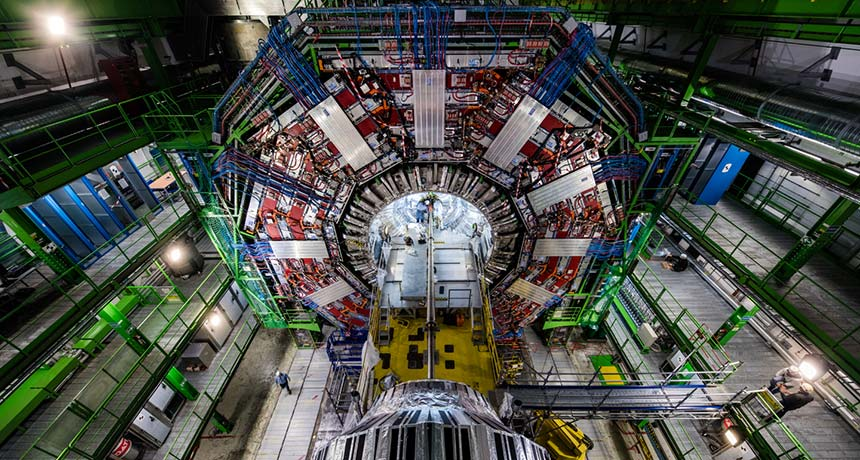
\includegraphics[width=\textwidth]{Images/CMS/CMS.jpg}
    \caption{The Compact Muon Solenoid}
    \label{fig:CMS_image}
\end{figure}

CMS is designed as a hermetic layered structure made of different technologies in order to detect different particles coming from proton-proton and heavy ion collisions delivered by the LHC. A slice of the CMS detector and its different technologies, and the different particles detected, is shown in Figure \ref{fig:CMS_PF}.

\begin{figure}[H]
    \centering
    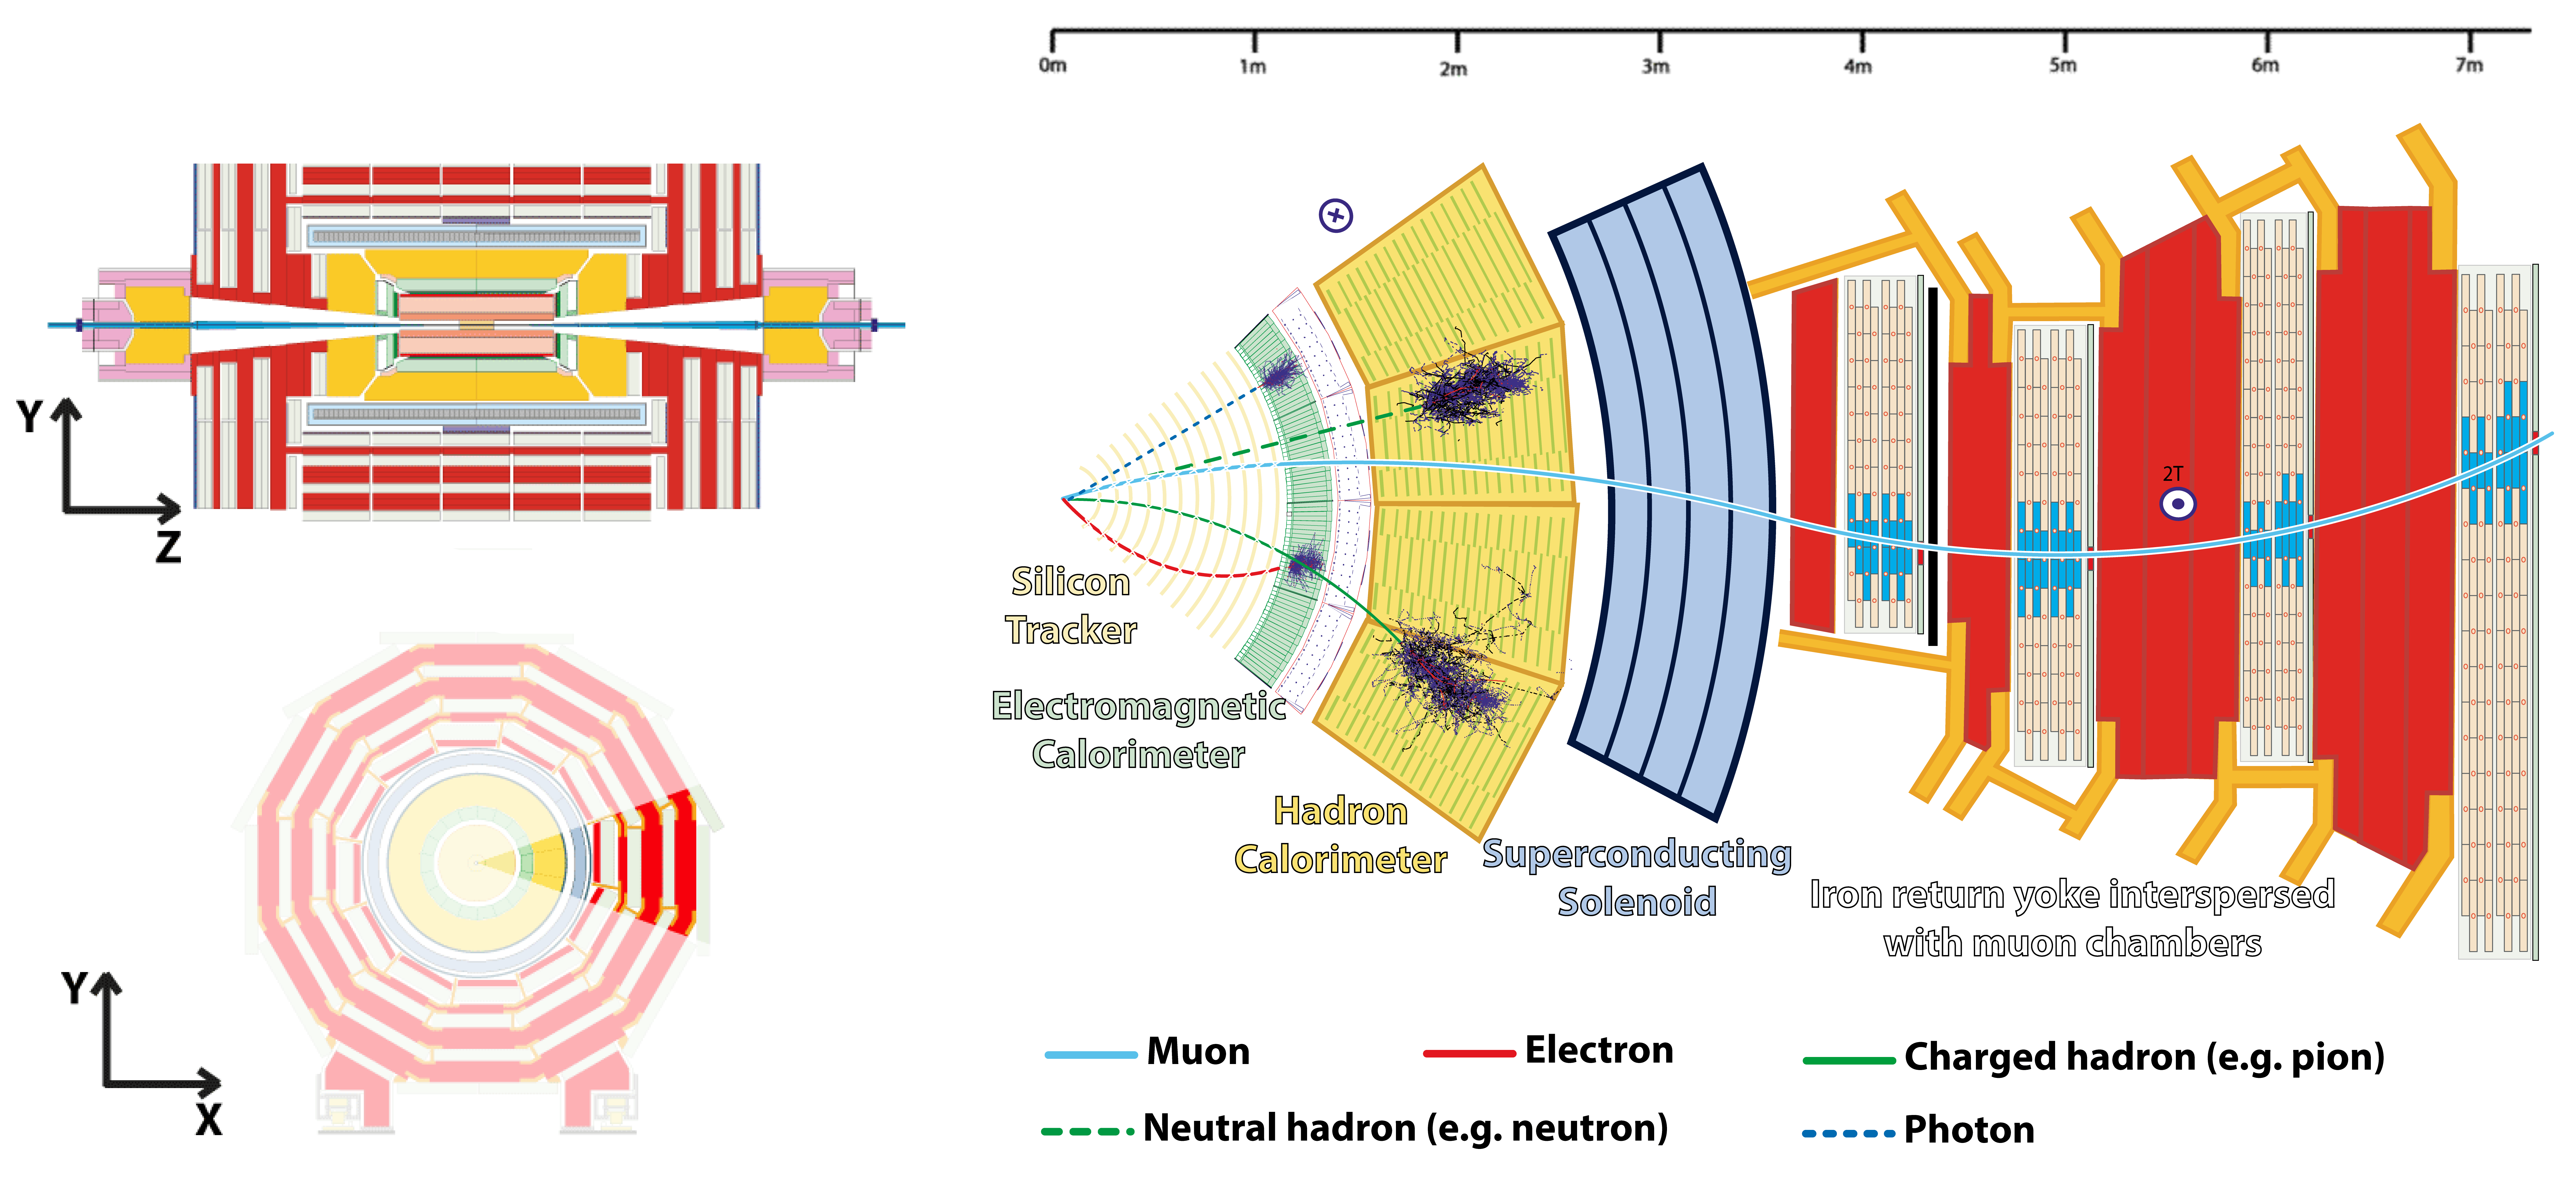
\includegraphics[width=\textwidth]{Images/CMS/CMS_PF.png}
    \caption{CMS detector technologies and particles detected.}
    \label{fig:CMS_PF}
\end{figure}

% Generic CMS description below:

% The central feature of the CMS apparatus is a superconducting solenoid of 6\unit{m} internal diameter, providing a magnetic field of 3.8\unit{T}. 
% Within the solenoid volume are a silicon pixel and strip tracker, a lead tungstate crystal electromagnetic calorimeter (ECAL), and a brass and scintillator 
% hadron calorimeter (HCAL), each composed of a barrel and two endcap sections. Forward calorimeters extend the pseudorapidity coverage provided by the barrel 
% and endcap detectors. Muons are measured in gas-ionization detectors embedded in the steel flux-return yoke outside the solenoid. A more detailed description 
% of the CMS detector, together with a definition of the coordinate system used and the relevant kinematic variables, can be found in Ref.~\cite{CMS:2008xjf}.

% Events of interest are selected using a two-tiered trigger system. The first level (L1), composed of custom hardware processors, uses information from the 
% calorimeters and muon detectors to select events at a rate of around 100\unit{kHz} within a fixed latency of about 4\mus~\cite{CMS:2020cmk}. The second level, 
% known as the high-level trigger (HLT), consists of a farm of processors running a version of the full event reconstruction software optimized for fast processing, 
% and reduces the event rate to around 1\unit{kHz} before data storage~\cite{CMS:2016ngn}.

% In the barrel section of the ECAL, an energy resolution of about 1\% is achieved for unconverted or late-converting photons in the tens of GeV energy range. 
% The energy resolution of the remaining barrel photons is about 1.3\% up to $\abs{\eta} = 1$, changing to about 2.5\% at $\abs{\eta} = 1.4$. In the endcaps, 
% the energy resolution is about 2.5\% for unconverted or late-converting photons, and between 3 and 4\% for the other ones~\cite{CMS:2015myp}.

% The diphoton mass resolution, as measured in $H\rightarrow\gamma\gamma$ decays, is typically in the 1--2\% range, depending on the measurement of the photon 
% energies in the ECAL and the topology of the photons in the event~\cite{CMS:2020xrn}.

% The integrated luminosities for the 2016, 2017, and 2018 data-taking years have 1.2--2.5\% individual uncertainties~\cite{CMS-LUM-17-003,CMS-PAS-LUM-17-004,CMS-PAS-LUM-18-002}, 
% while the overall uncertainty for the 2016--2018 period is 1.6\%.

\subsection{Tracker}
The CMS tracker is the innermost layer of CMS, and is composed of silicon pixel and strip trackers. The main purpose of the tracker is to detect tracks left by electrically charged particles. These tracks are used to measure particle momentum, corresponding to the track's radius. Additionally, the tracker is used to identify the sign of the particle's charge, and is crucial for identifying the vertex of hard interactions from LHC collisions. The tracker is the most sensitive of the CMS sub-detectors, and is subject to the brunt of radiation produced by LHC collisions.  

\subsubsection{Pixel tracker} \label{sec:PIXEL}

The innermost layer of the CMS detector, and first layer of the CMS tracker, is the pixel tracker. This pixel tracker is composed of silicon sensors, of which there were initially about 65 million individual pixel readout channels in 2016. After the first full year of Run 2 data taking in 2016, the pixel detector was upgraded to the Phase-I pixel detector \cite{PhaseI_Pixel} in order to maintain performance following the upgrade of the LHC during the first Long Shutdown (LS1) from 2013-14, from which an instantaneous luminosity larger than the original pixel detector design was produced. The Phase-I pixel detector was installed during the 2016 Year End Technical Stop (YETS), which lasted from December 2016 to April 2017. After its installation, the Phase-I pixel detector, now containing about 124 million individual channels, was used during the 2017 and 2018 data-taking periods of Run 2.

The pixel tracker is composed of the Barrel (BPIX) and Forward (FPIX) pixel detectors, which result in a combined pseudorapidity region for particle detection of $|\eta| < 2.5$. A layout of the Phase-I pixel detector, and a comparison to the original design, is shown in Figure \ref{fig:Pixel_Tracker}. 

% \begin{figure}[H]
%     \centering % trim=left botm right top
%     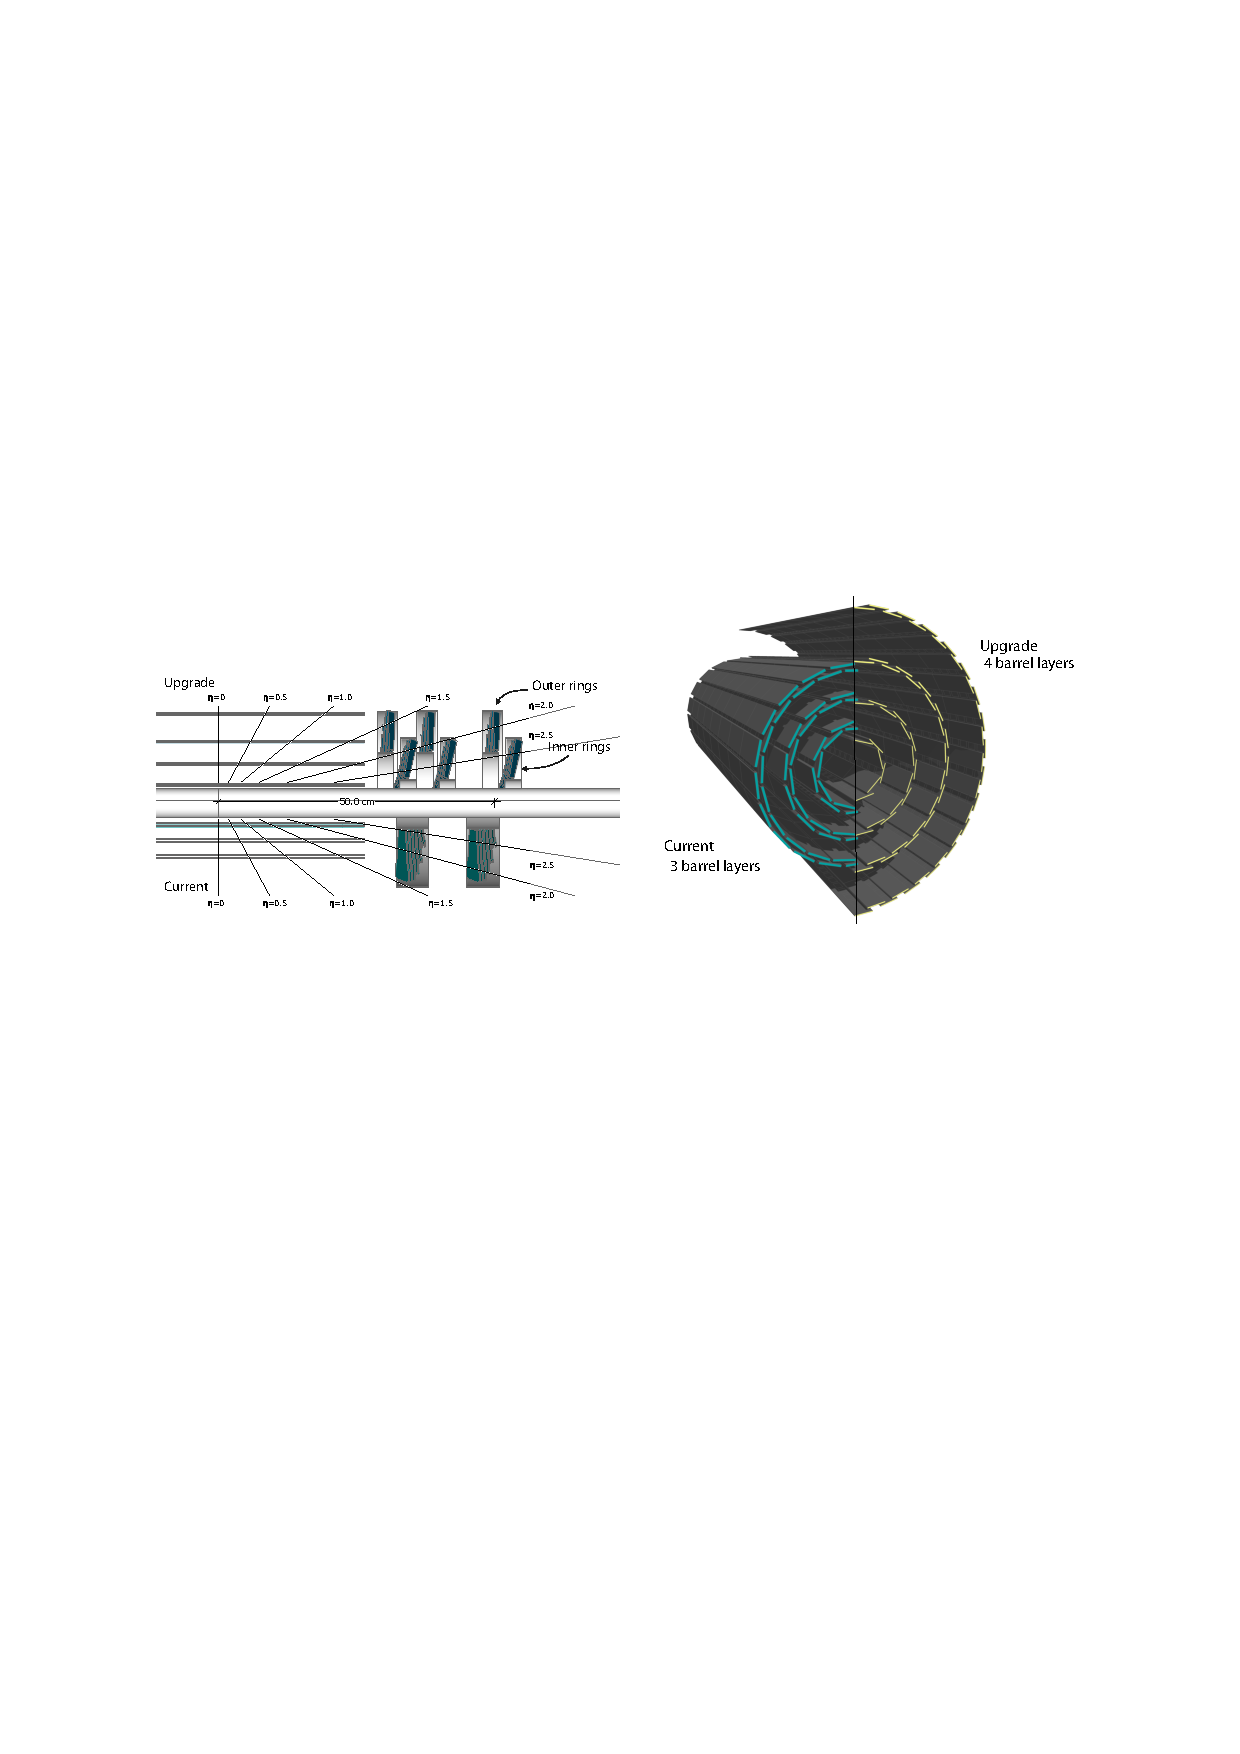
\includegraphics[clip, trim=0cm 0cm 0cm 6cm , width=\textwidth]{Images/CMS/Tracker/Tracker_Phase_Compare.pdf}
%     \caption{The Phase-I CMS pixel detector (upper), compared to its original design (lower).}
%     \label{fig:Pixel_Tracker}
% \end{figure}

\begin{figure}[H]
    \centering % trim=left botm right top
    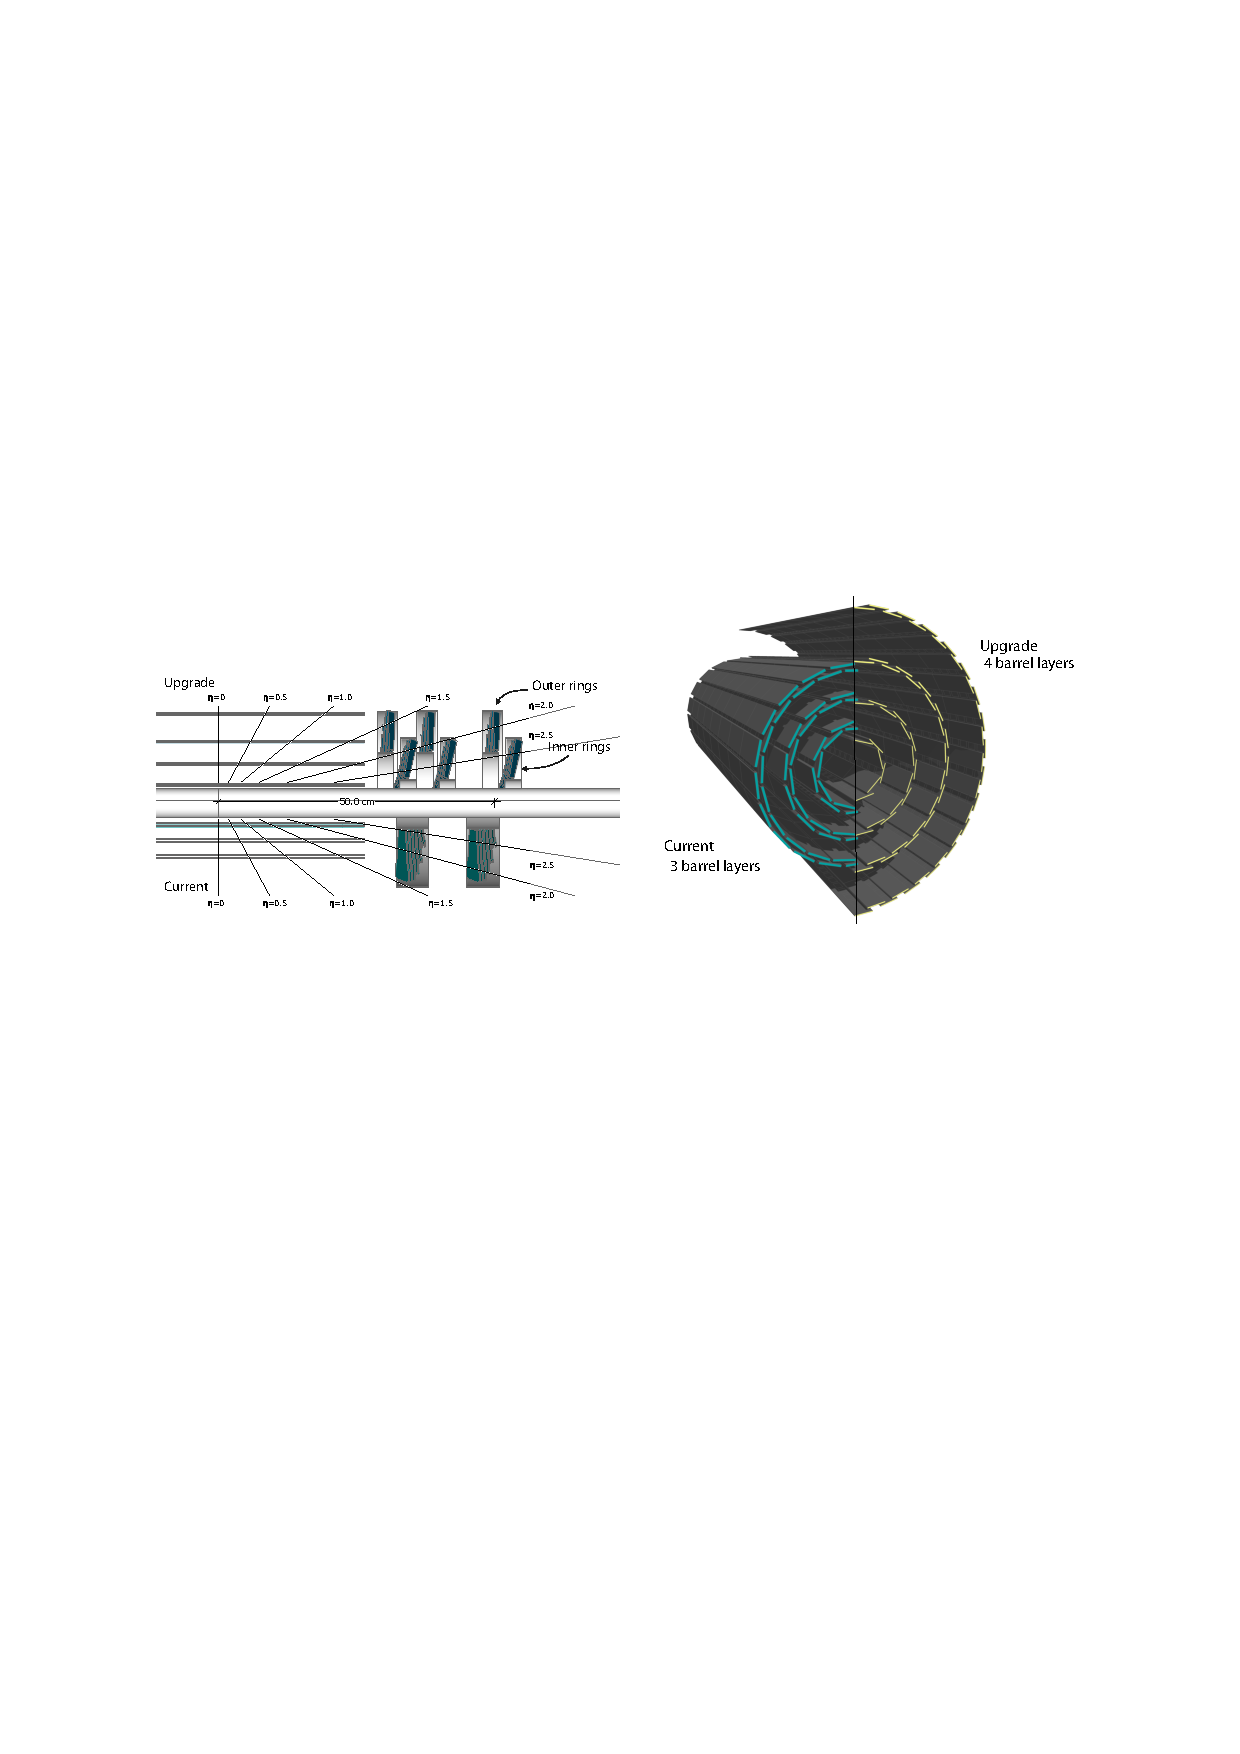
\includegraphics[width=\textwidth]{Images/CMS/Tracker/Tracker_Phase_Compare.pdf}
    \caption{The Phase-I CMS pixel detector (``Upgrade"), compared to its original design (``Current").}
    \label{fig:Pixel_Tracker}
\end{figure}

It can be seen that the main additions to the original CMS pixel detector are the addition of a layer in BPIX, and the addition of several disks in FPIX. Half of the BPIX system during production is shown in Figure \ref{fig:BPIX_Half}. In this image, the four half-circles concentric to the center of the image correspond to the four layers, L1-4. 

\begin{figure}[H]
    \centering
    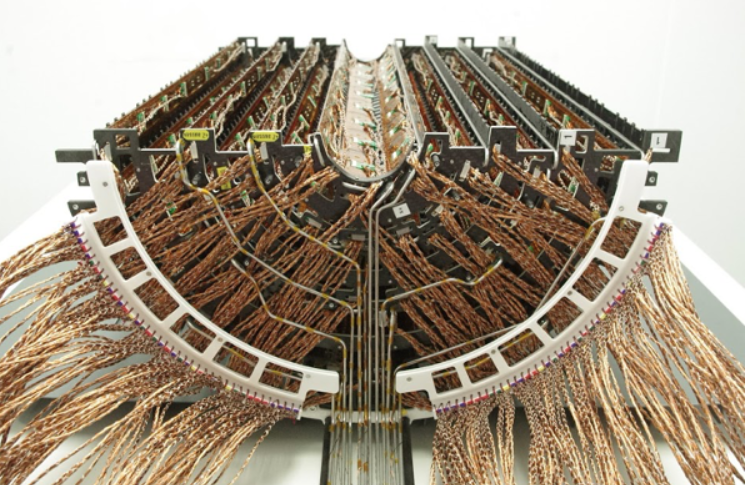
\includegraphics[width=0.7\textwidth]{Images/CMS/Tracker/BPIX.png}
    \caption{Half of the Phase-I BPIX.}
    \label{fig:BPIX_Half}
\end{figure}

The Phase-I pixel detector was able to deliver its expected performance, as shown in Figure \ref{fig:PIX_HitEfficiency}. 

\begin{figure}[H]
    \centering
    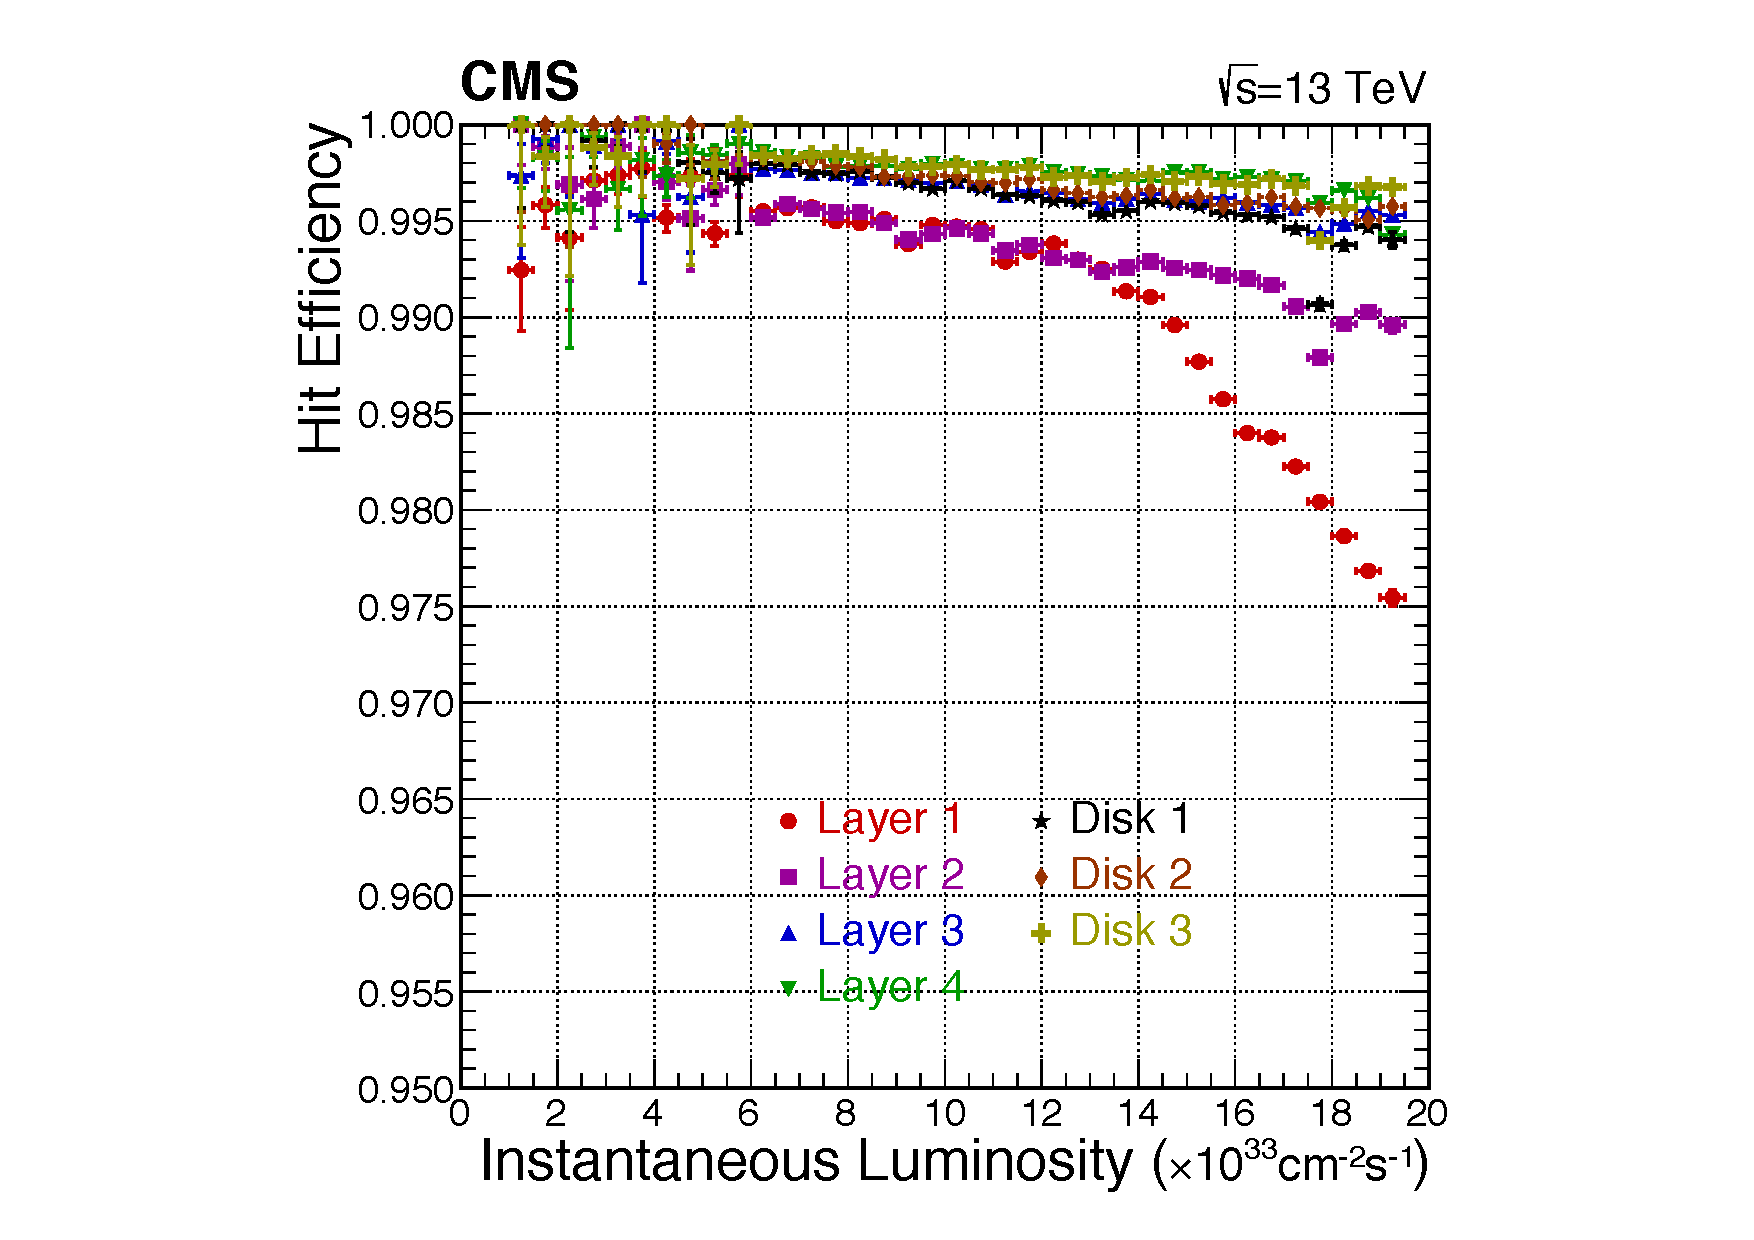
\includegraphics[width=\textwidth]{Images/CMS/Tracker/Pixel_HitEfficiency.pdf}
    \caption{Pixel hit efficiency during 2018.}
    \label{fig:PIX_HitEfficiency}
\end{figure}

The hit efficiency is shown as a function of different instantaneous luminosities during the 2018 data-taking year of Run 2, where higher values correspond to a higher number of simultaneous interactions, and therefore harsher data-taking conditions. Hit efficiency is defined as the probability that a cluster of pixel hits corresponds to an extrapolated track. Layers 1-3 of BPIX, and the entire FPIX were able to maintain hit efficiencies around 99\% even for large instantaneous luminosity values of 2*$ 10^{34}$cm$^{-2}$s$^{-1}$. Additionally, the L1 hit efficiency, which suffers the most from the harsh data-taking conditions at it is closest to the interaction region, begins to drop around 1.4*$10^{34}$cm$^{-2}$s$^{-1}$ down to about 97.5\% at 2cm$10^{34}^{-2}$s$^{-1}$. However, this performance is greater than what would have been expected from the original pixel tracker which ran during 2016. 

This is an example of a detector upgrade which was unforeseen but deemed necessary to implement, in response to the data-taking conditions presented to CMS based on collisions delivered by the LHC.

\subsubsection{Strip tracker}

% https://pos.sissa.it/309/013/pdf
% https://twiki.cern.ch/twiki/bin/view/CMSPublic/DPGResultsTRK

The second layer of the CMS detector, and outer portion of the CMS tracker, is the strip tracker. A view of one quarter of the Phase I strip tracker used during Run 2 can be seen in Figure \ref{fig:Strip_Tracker}. 

\begin{figure}[H]
    \centering
    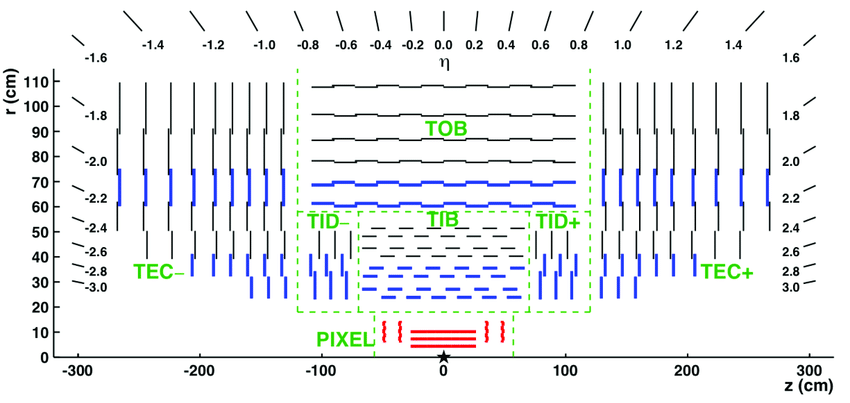
\includegraphics[width=0.7\textwidth]{Images/CMS/Tracker/upper-Schematic-view-of-the-CMS-tracker-detector-1-and-lower-closeup-view-of-the.png}    
    \caption{A view of half of the CMS strip detector in the r-z plane of CMS.}
    \label{fig:Strip_Tracker}
\end{figure}

The CMS strip tracker is composed of 15,148 silicon sensors which are spread over several partitions to cover different regions around the collision point: The Tracker Outer Barrel (TOB), Tracker Inner Barrel (TIB), Tracker Inner Disks (TID) with a plus and minus side, and Tracker Endcaps (TEC) which have modules on the plus and minus side. As shown in the diagram, the strip tracker surrounds the pixel tracker described in Section \ref{sec:PIXEL}. 

The strip tracker performs the same task as the pixel tracker, namely recording hits from electromagnetically charged particles in order to track their movement - a vital task for measuring particle $p_{T}$, identifying interaction vertices, and identifying jets from quark/gluon hadronization. The pixel and strip measurements are combined in order to obtain more accurate track measurements.  

During Run 2, the strip tracker maintained an excellent signal over noise ratio, and held a very stable percentage of problematic channels during Run 2, shown in Figure \ref{fig:Run2_StripTracker}.

\begin{figure}[H]% 
    \setcounter{subfigure}{0} % reset subcaption counter to 0 (a) 
    \centering
    \subfloat[2017 Signal over noise of TIB ]{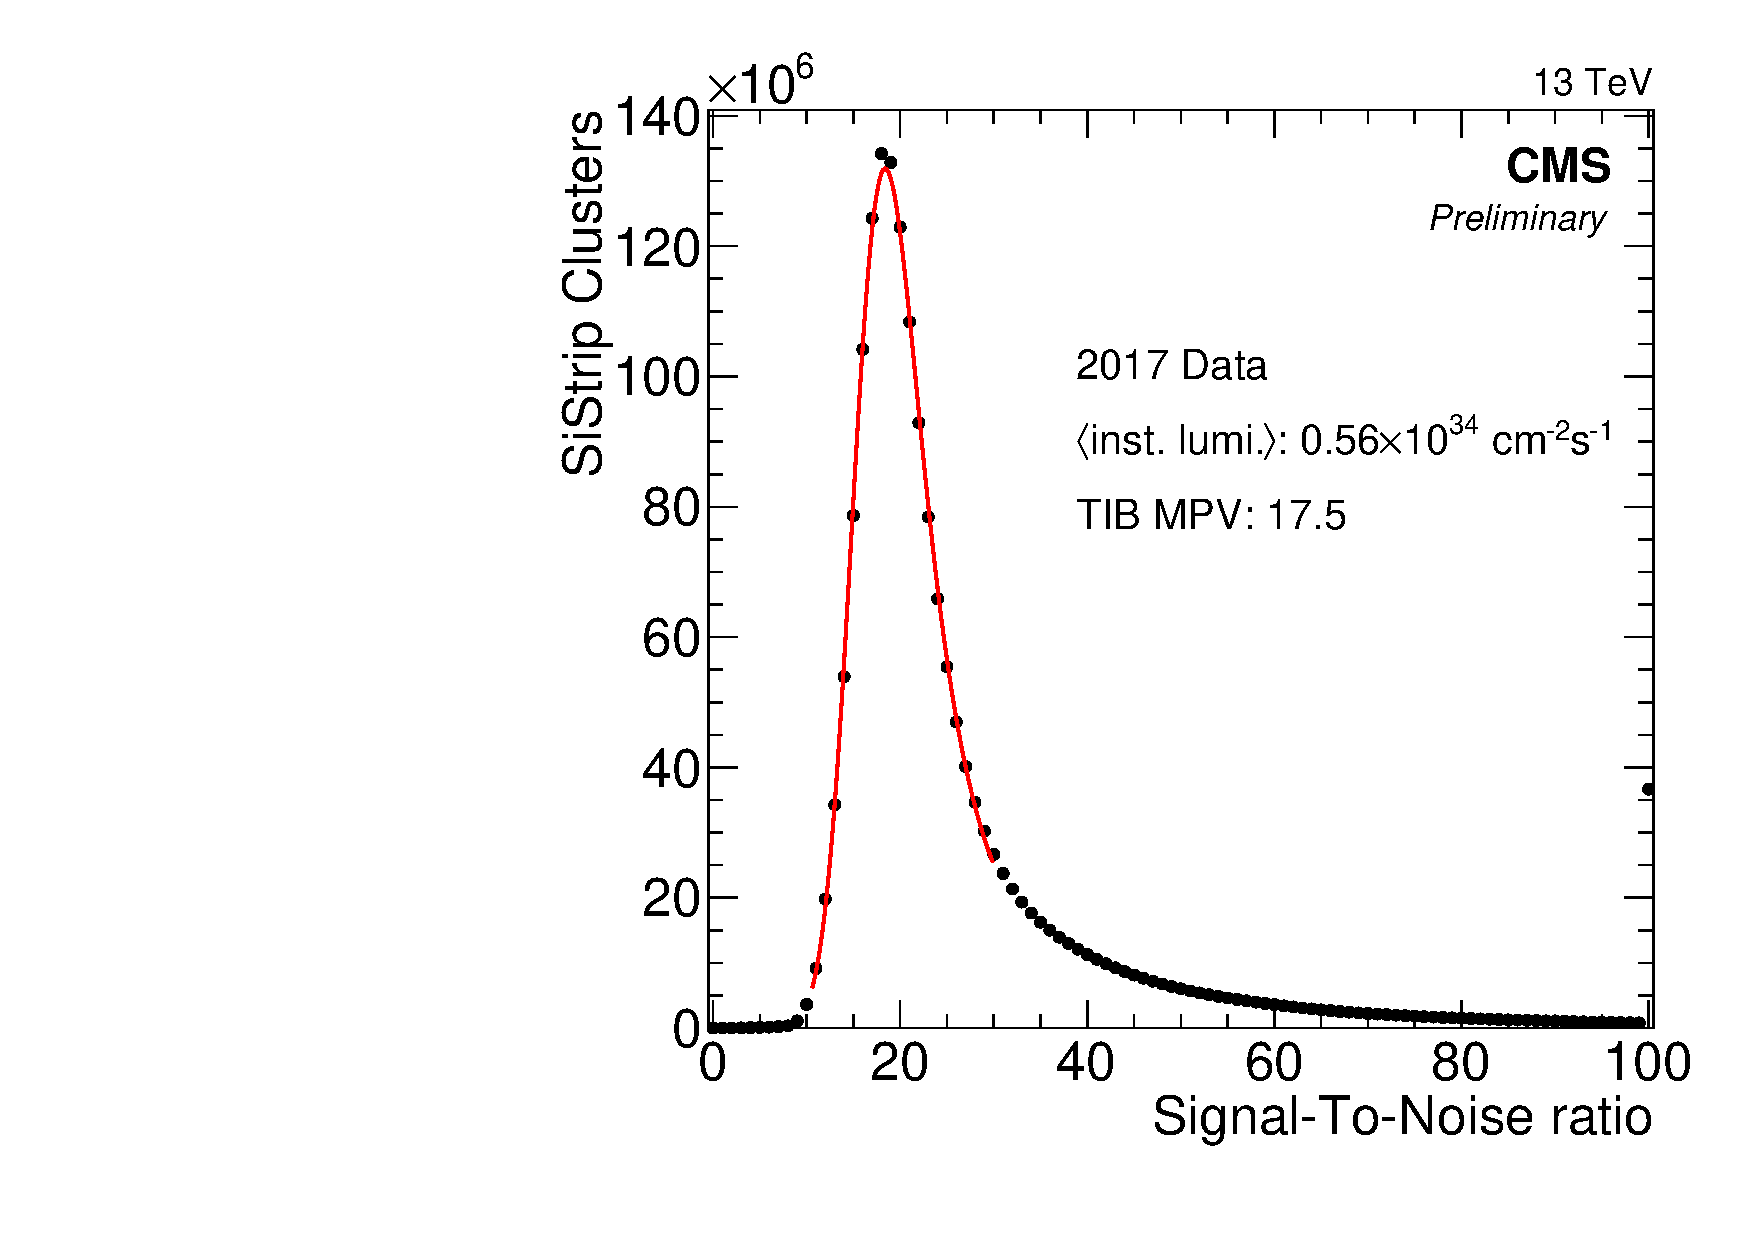
\includegraphics[height=.25\textheight]{Images/CMS/Tracker/StripTracker_SON_TIB_SOverN_run296786_2017A.pdf}}%
    \qquad
    \subfloat[Run 2 problematic channel fraction ]{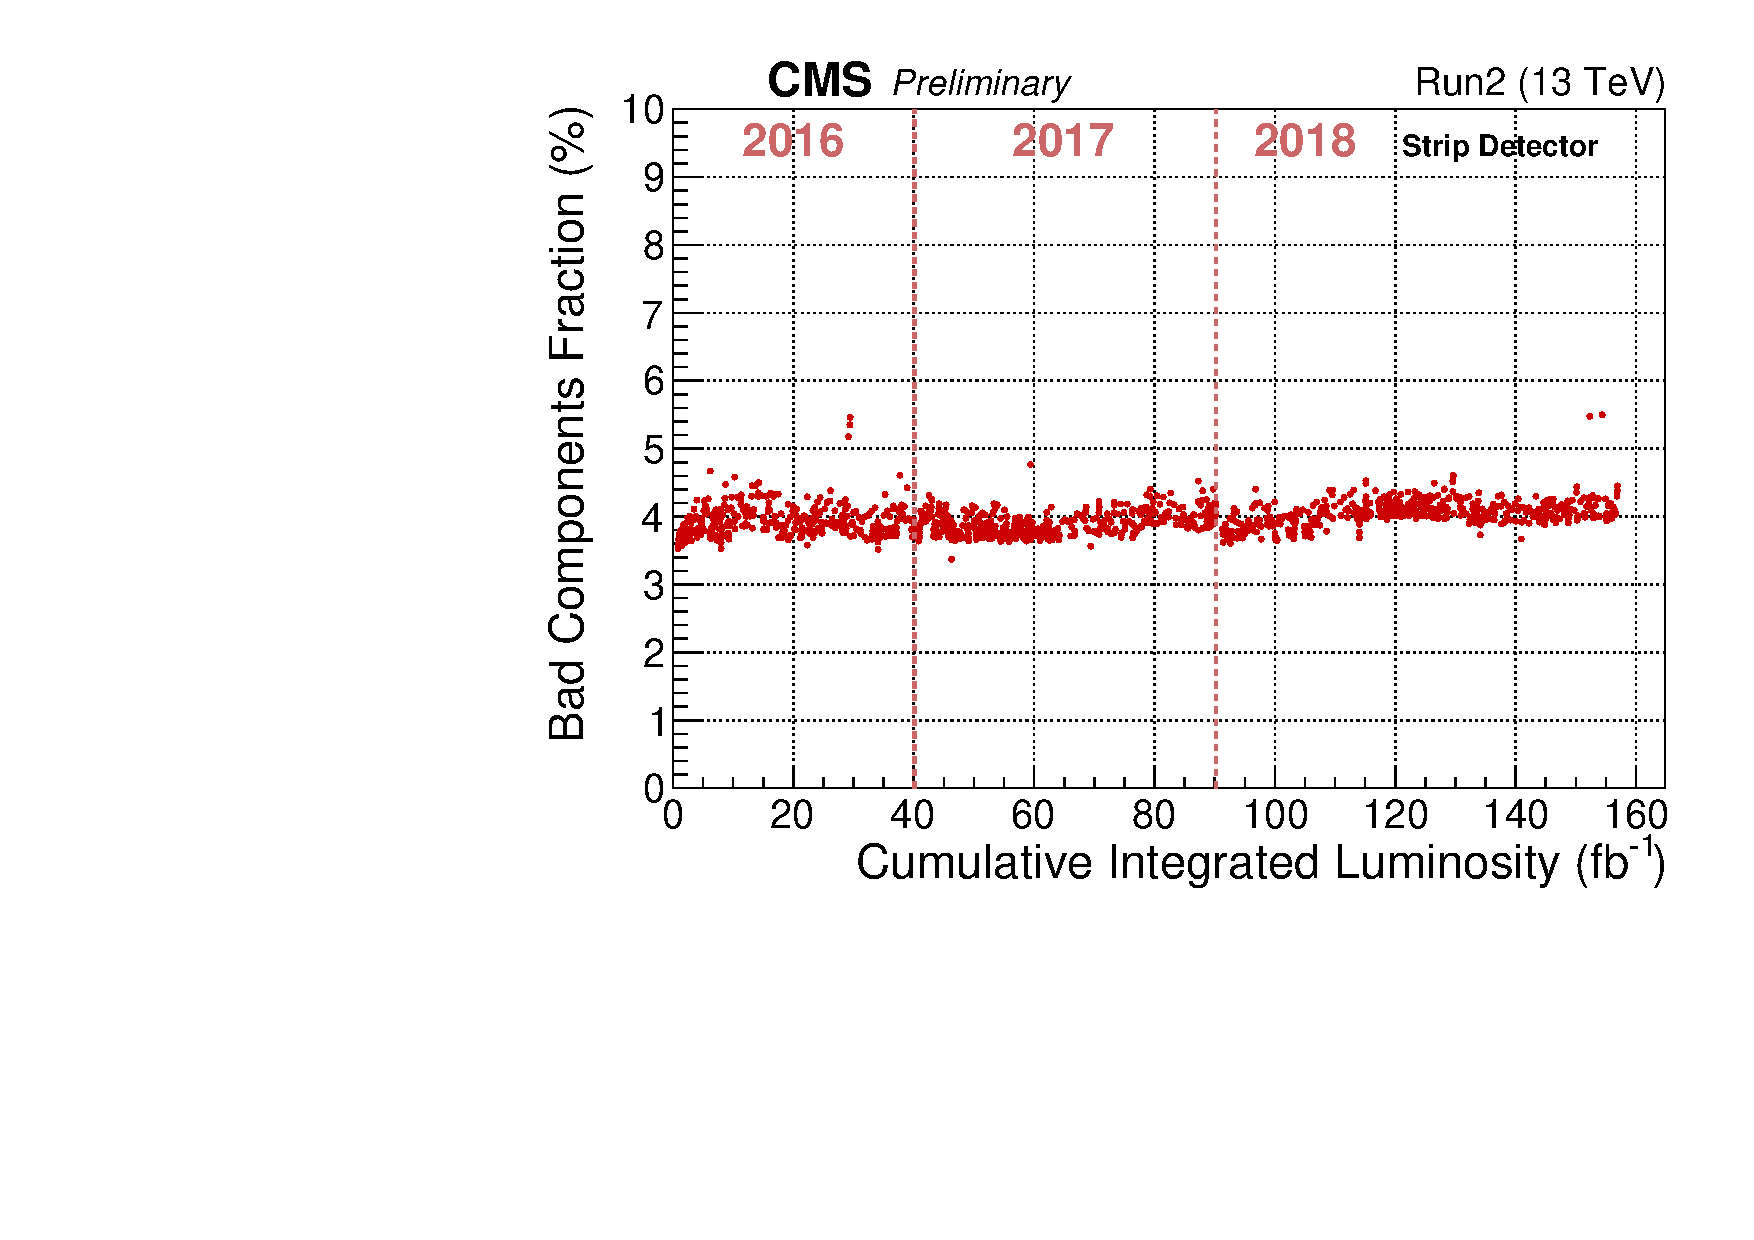
\includegraphics[height=.25\textheight]{Images/CMS/Tracker/run2_stripBadComponent_All.pdf}}%
    \caption{Run 2 strip tracker performance.} \label{fig:Run2_StripTracker}
\end{figure}  

In 2017, TIB had an excellent MPV (Most probable value) of 17.5 as a signal-to-noise ratio, indicating good signal detection in the strip tracker partition closest to the CMS interaction point. Additionally, over the course of Run 2 operations the percentage of bad components remain stable at about 4\% even after receiving the full Run 2 intergrated luminosity, highlighting the robustness of the detector. 

\subsection{Calorimeters}
The two calorimeters contained within the CMS detector are the Electromagnetic Calorimeter (ECAL), and the Hadronic Calorimeter (HCAL). A description of ECAL is provided in Section \ref{sec:ECAL}, and a description of HCAL is provided in Section \ref{sec:HCAL}. 

% \subsubsection{The Electromagnetic Calorimeter}\label{sec:ECAL}

% The CMS Electromagnetic Calorimeter is the second layer of the CMS detector, with respect to the interaction point of collisions produced by the LHC. In this Chapter, the CMS ECAL will first be introduced in Section \ref{sec:ECAL_Introduction}. In Section \ref{sec:ECAL_TPG}, the method of ECAL Trigger Primitive Generation as input to the CMS L1 trigger will be described. In Section \ref{sec:DW}, the development and commissioning of a new ECAL feature known as ``Double Weights" will be described, and in Section \ref{sec:ECAL_Operations} the various ECAL operations teams and their responsibilities will be described.  

% \section{Introduction} \label{sec:ECAL_Introduction}

\subsubsection{The Electromagnetic Calorimeter}\label{sec:ECAL}

The CMS ECAL is a homogeneous crystal calorimeter composed of 75,848 PbWO$_{4}$ (lead tungstate) crystals that measures the energy of photons and electrons with high precision. The ECAL is composed of a barrel (EB) containing 61,200 crystals and covering the pseudorapidity $\eta$ region $|\eta| < 1.479$, and two endcaps (EE) containing 14,648 crystals and extending the coverage up to $|\eta| = 3$. Accurately measuring the energy and position information of electrons and photons is vital for an extensive array of physics analyses, in particular the decays of the Higgs boson in the two photon and ZZ to 4 leptons channels, considered the ``golden channels\,'' in the experimental discovery of the Higgs boson. The ECAL is supported by an additional subsystem called the ECAL Preshower (ES), located in front of each ECAL endcap. ES is composed of lead and silicon sensors, and is meant to improve two-photon separation, i.e. determine whether photons came from pion decays rather than from Higgs boson, or other interesting decays. The layout and geometry of the CMS ECAL and ES are shown in Figures \ref{fig:ECAL_Partitions} and \ref{fig:ECAL_Geometry}. Images of the EB and half of an EE endcap are shown in Figure \ref{fig:ECAL_Images}. 

\begin{figure}[H]
    \centering
    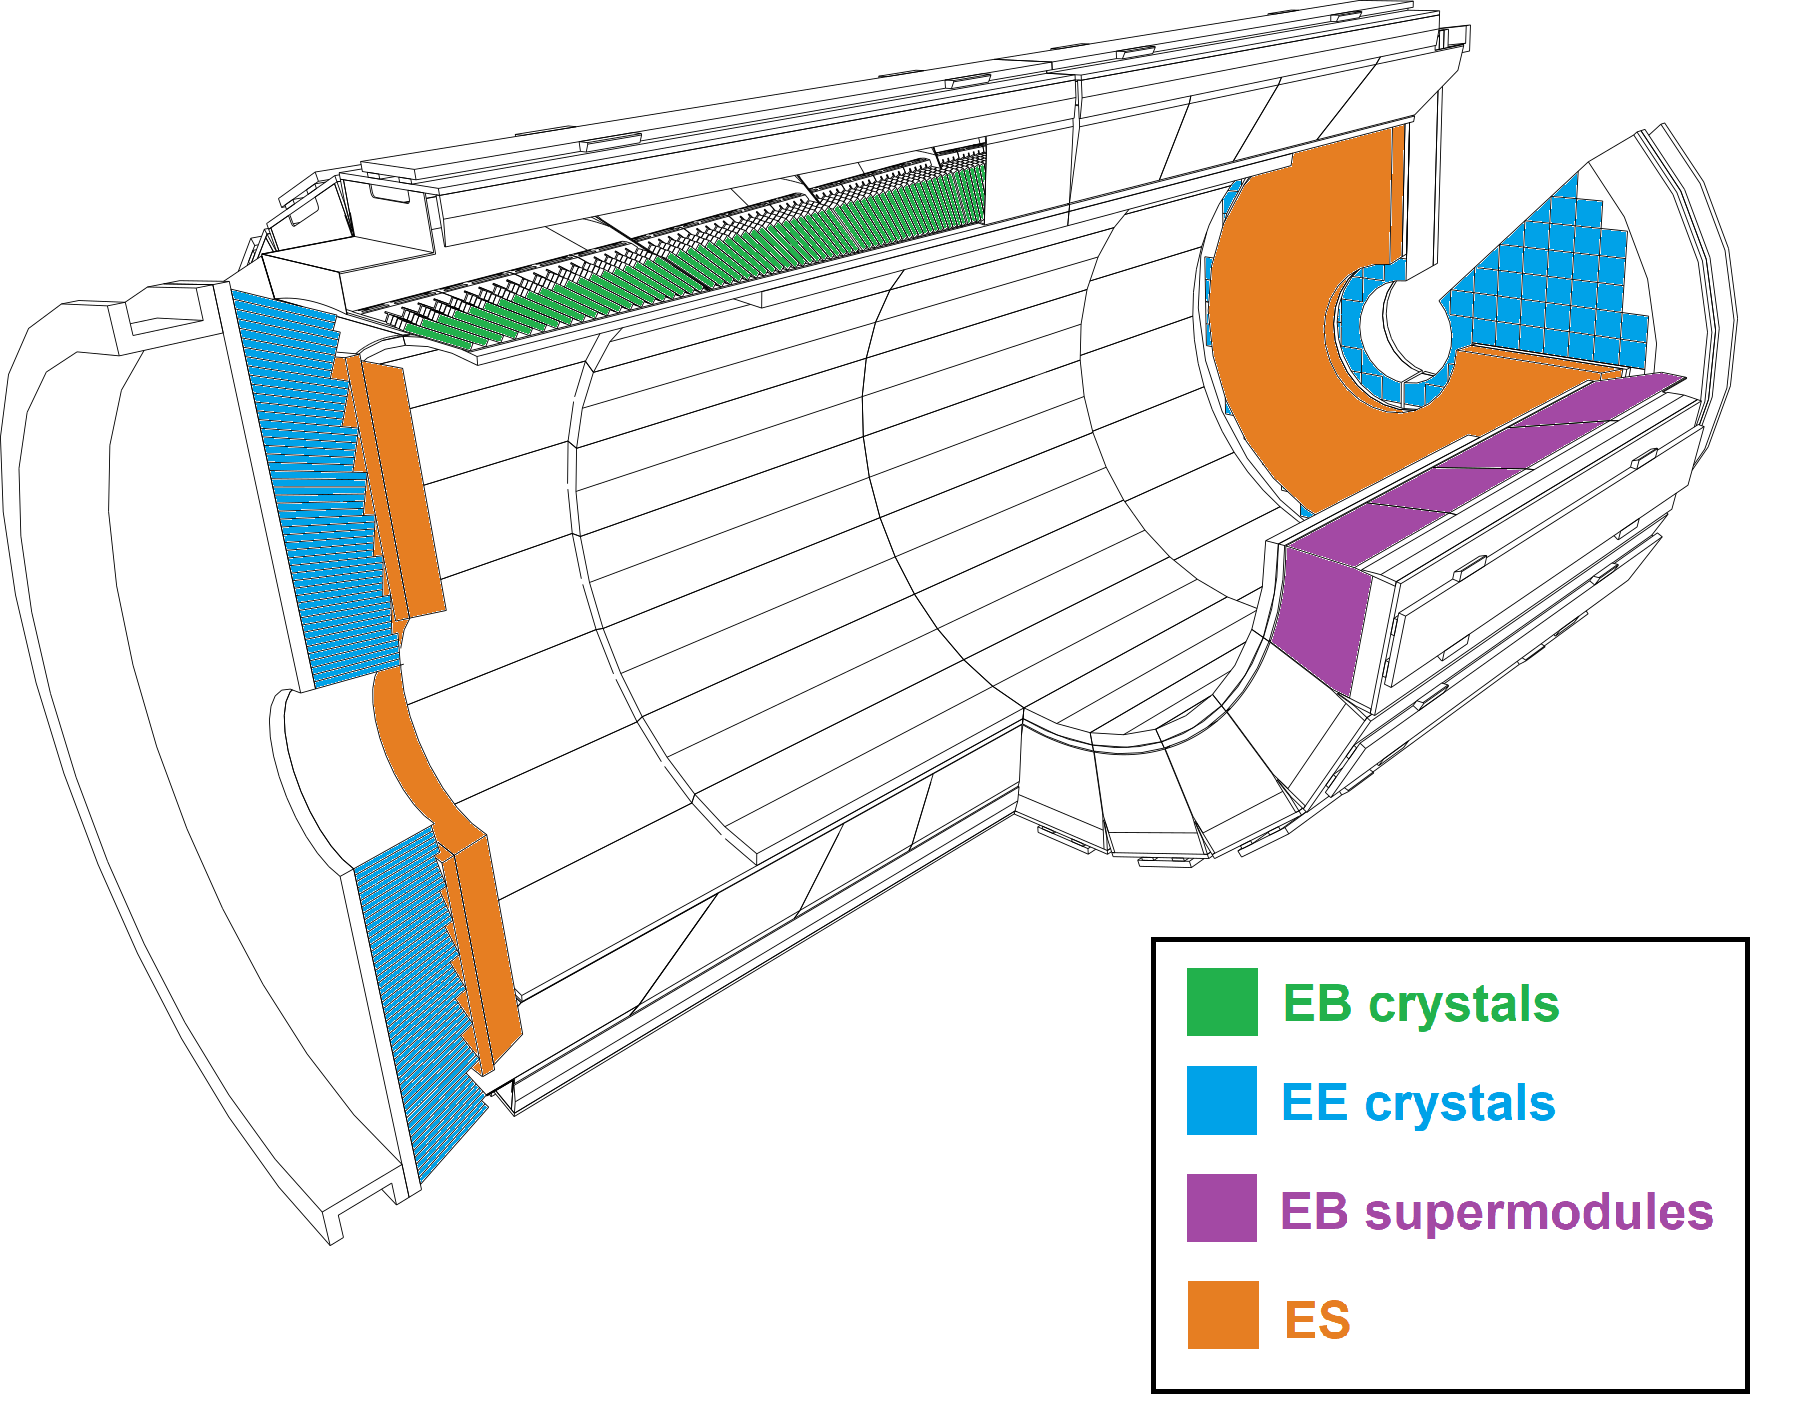
\includegraphics[width=0.65\textwidth]{Images/ECAL/Introduction/ECAL_ES_Diagram_colored.png}    
    \caption{CMS ECAL and ES partitions.}
    \label{fig:ECAL_Partitions}
\end{figure}

\begin{figure}[H]
    \centering
    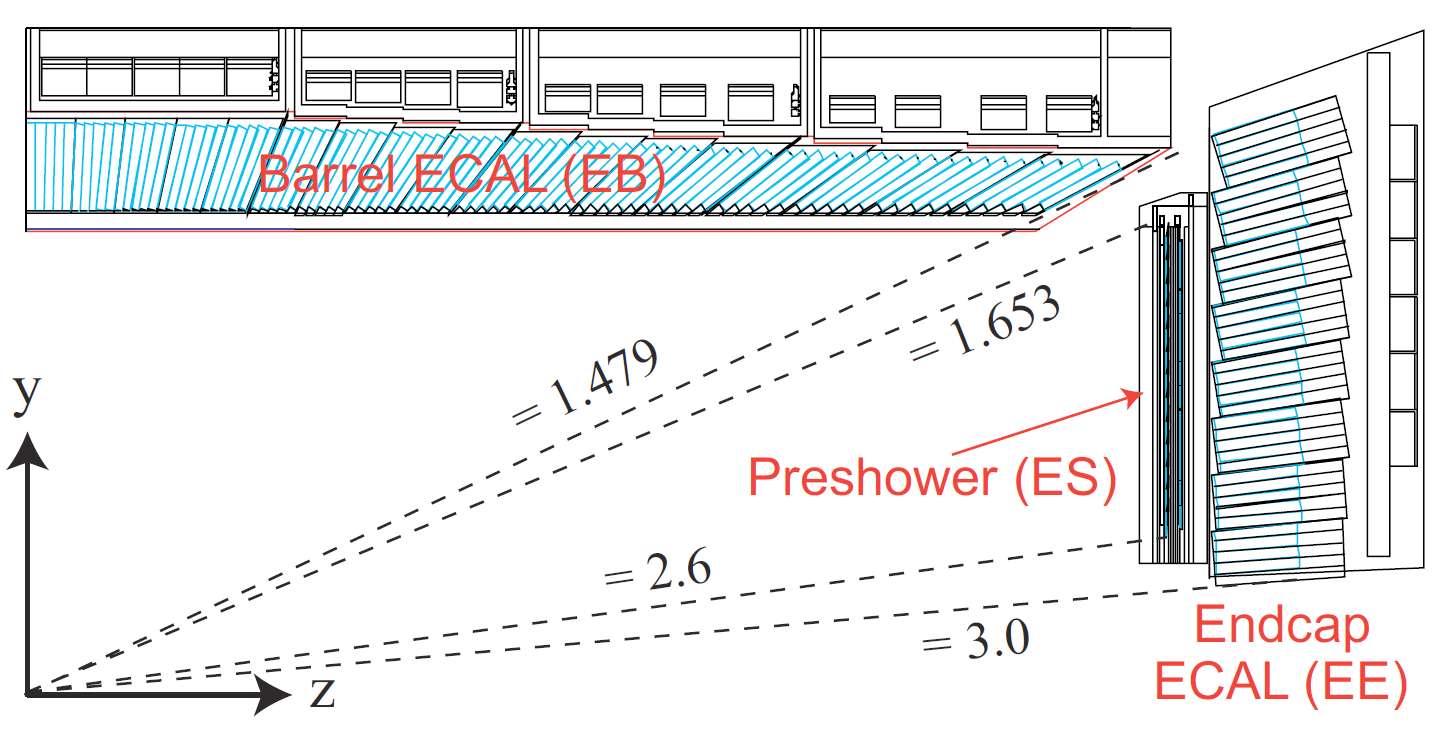
\includegraphics[width=0.65\textwidth]{Images/ECAL/Introduction/ECAL_Diagram.png}    
    \caption{Geometric coverage of the CMS ECAL and ES.}
    \label{fig:ECAL_Geometry}
\end{figure}

% https://cms.cern/detector/measuring-energy/ecal-preshower

\begin{figure}[H]%
    \setcounter{subfigure}{0}
    \centering
    \subfloat[ECAL barrel]{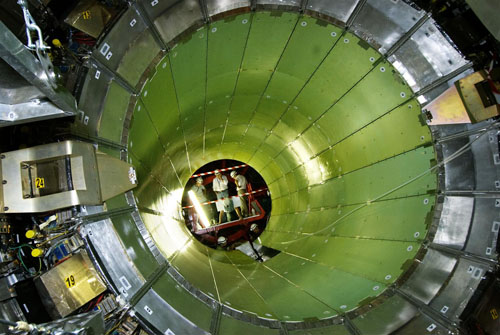
\includegraphics[width=.4\textwidth]{Images/ECAL/Introduction/EB_Image.jpg}}%
    \hfill
    \subfloat[Half of an ECAL endcap]{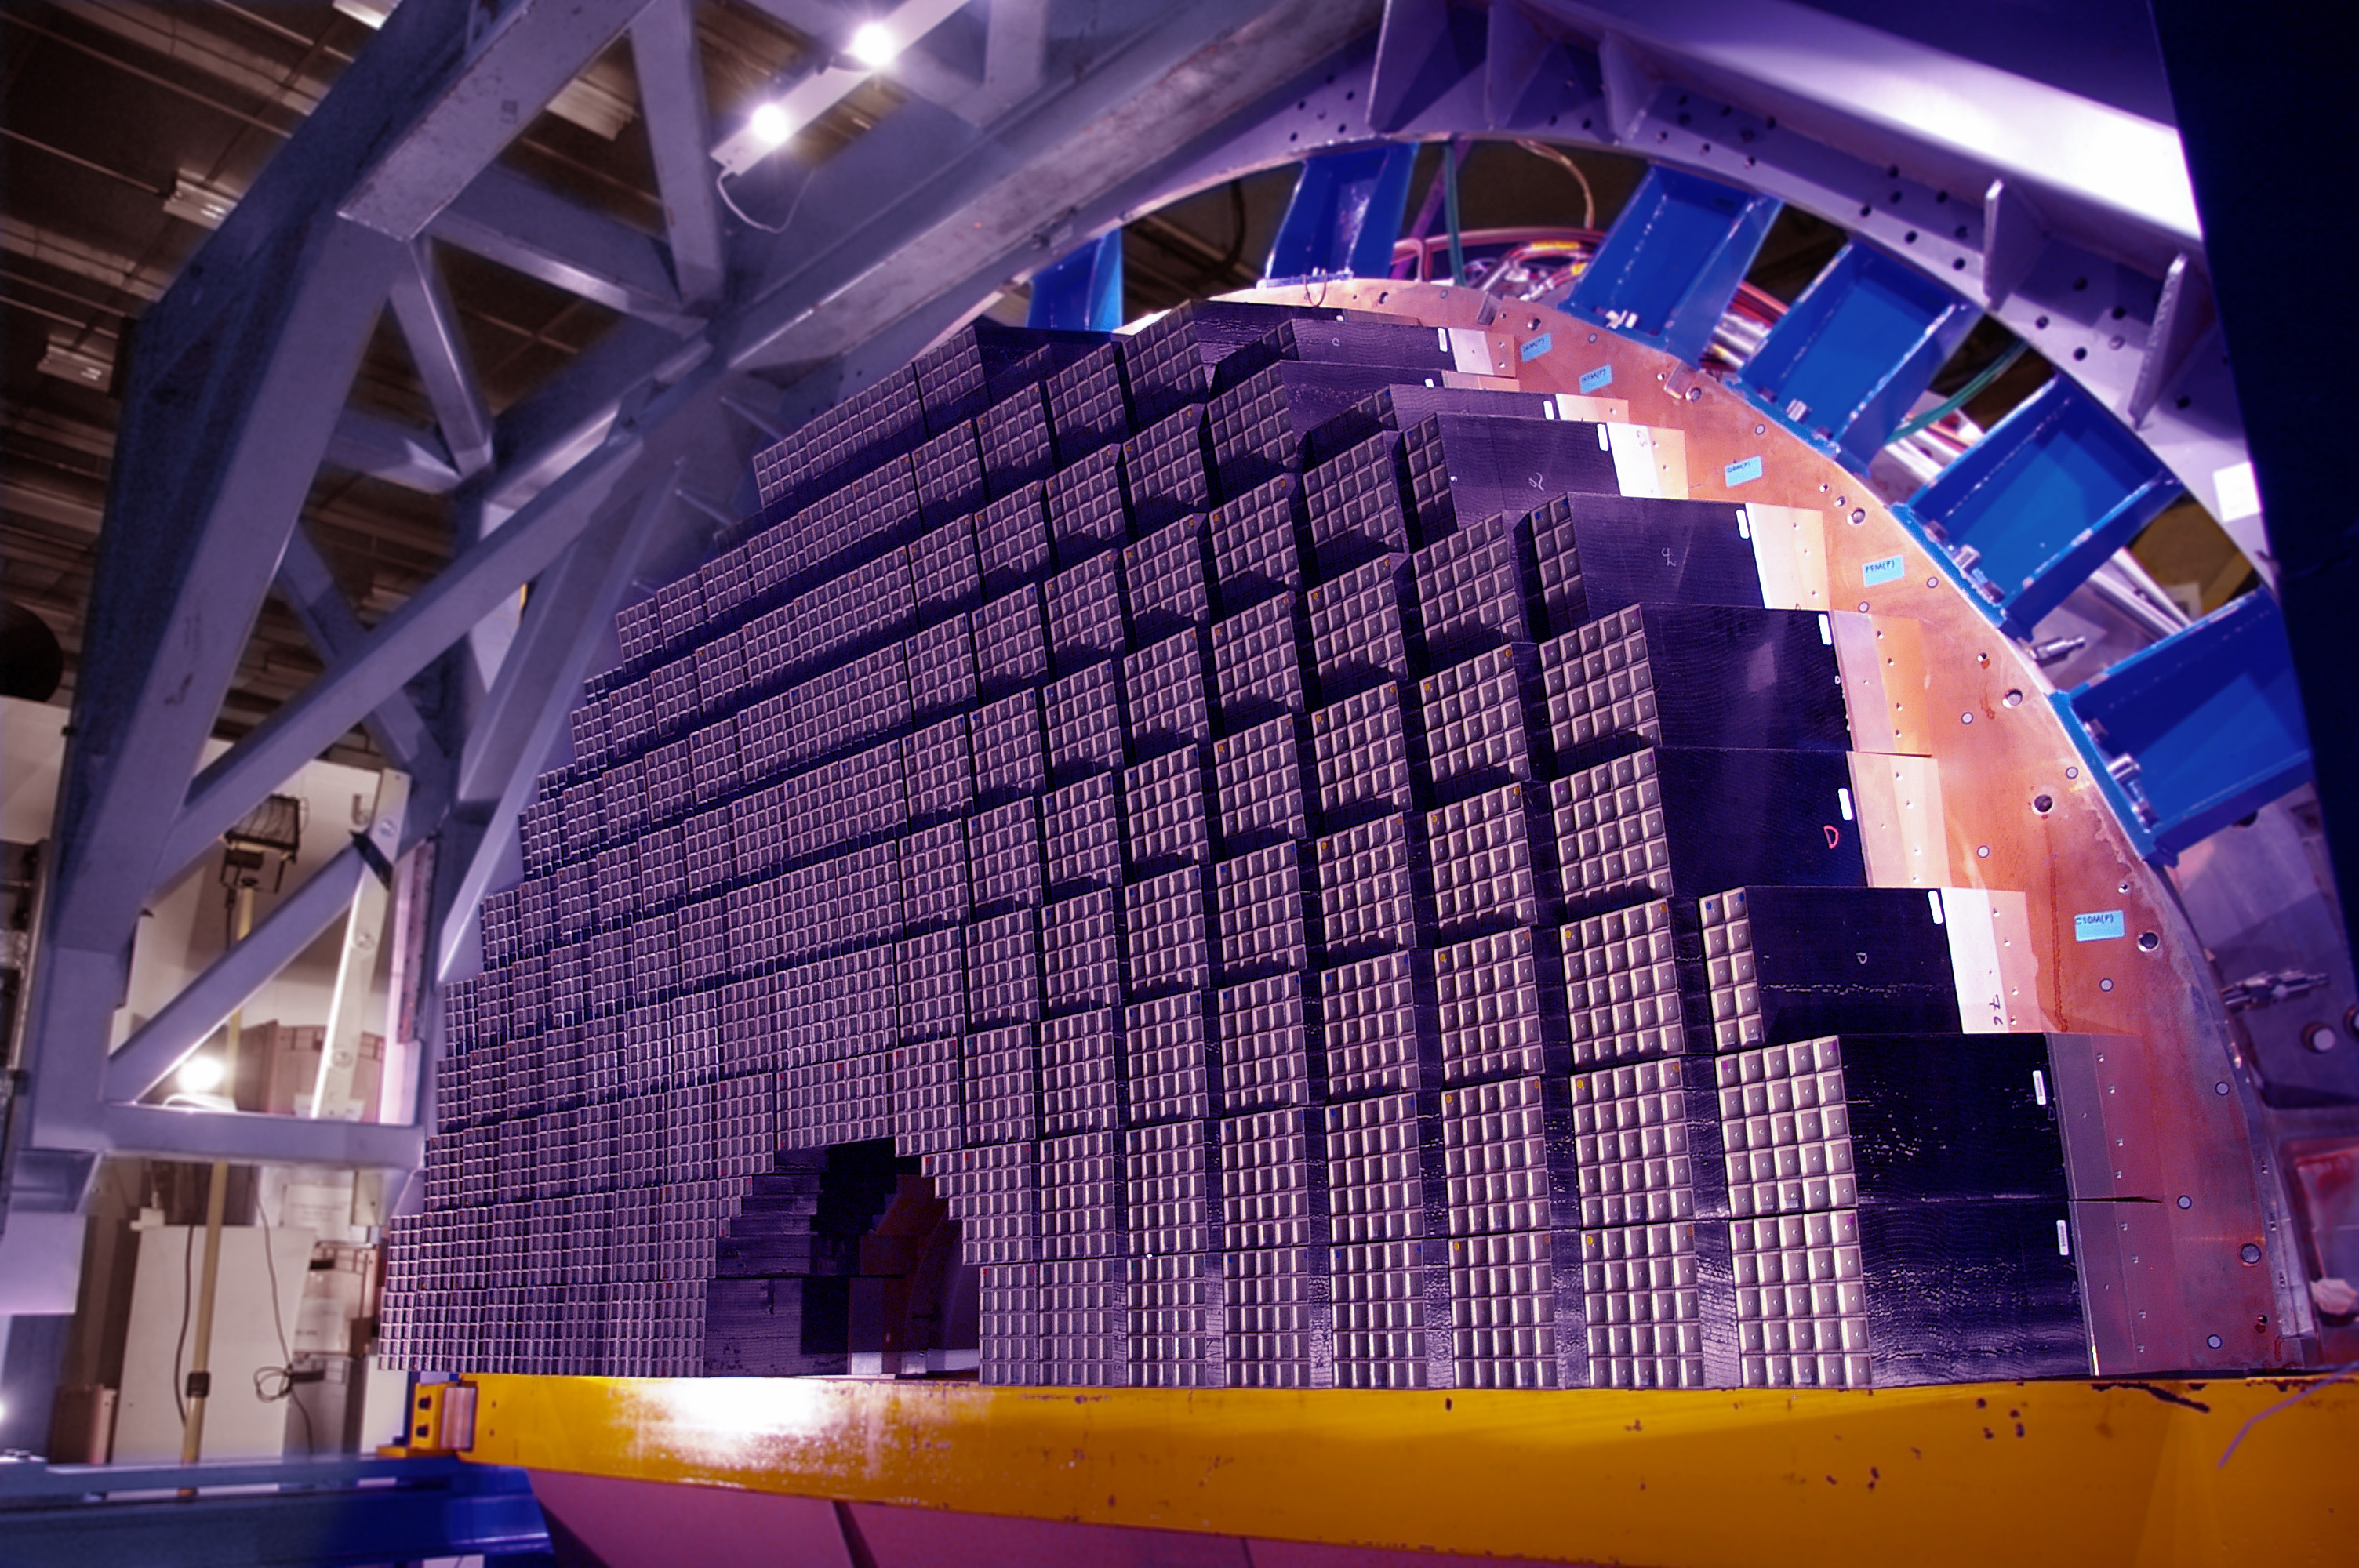
\includegraphics[width=.4\textwidth]{Images/ECAL/Introduction/EE_Half.jpg}}%
    \caption{Images of the CMS ECAL. \label{fig:ECAL_Images}}%
\end{figure}  

The basis of detection at ECAL is an electromagnetic shower. As a high energy electron or photon approaches ECAL, the electron will emit a photon as bremsstrahlung radiation, and the photon will pair produce to an electron-positron pair in the presence of massive detector material. The resulting photons, electrons, and positrons from this initial process will then perform the same types of processes as a cascade of particles is produced in the ECAL crystals. This is shown as a diagram in Fig. \ref{fig:Photon_Shower} for a photon initiating a shower, Fig. \ref{fig:Electron_Shower} for an electron initiating a shower, and is visualized as a simulation in Fig. \ref{fig:Simulated_Shower}. 

\begin{figure}[H]
    \centering
    
\includegraphics[width=0.7\textwidth]{Images/ECAL/Introduction/Photon_Shower.png}    
    \caption{Diagram form of a photon initiating an electromagnetic shower via pair production of an electron-positron pair.}
    \label{fig:Photon_Shower}
\end{figure}

\begin{figure}[H]
    \centering
    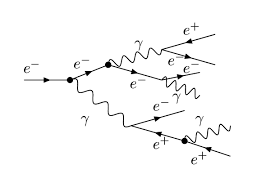
\includegraphics[width=0.7\textwidth]{Images/ECAL/Introduction/Electron_Shower.png}    
    \caption{Diagram form of an electron initiating an electromagnetic shower via bremsstrahlung radiation.}
    \label{fig:Electron_Shower}
\end{figure}

\begin{figure}[H]
    \centering
    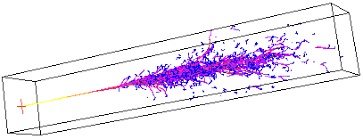
\includegraphics[width=0.7\textwidth]{Images/ECAL/Introduction/EM_Crystal_Shower.png}    
    \caption{Simulated electromagnetic shower inside a material.}
    \label{fig:Simulated_Shower}
\end{figure}

In ECAL, this EM shower leads to scintillation in its lead tungstate crystals, producing light that is read by photodetectors on the back of the crystals. The EB uses APDs (avalanche photodiodes), and the endcaps use VPTs (vacuum phototriodes) to convert scintillation light into an electrical signal. Digitized samples of ECAL are taken every 25 ns, and through a series of calibrations, the samples can be converted into an energy in GeV. An image of an EE crystal with its attached VPT is shown in Figure \ref{fig:ECAL_XTAL}.

% https://indico.cern.ch/event/1002959/contributions/4211462/attachments/2192922/3706736/EGM_Seminar_21-02-18.pdf

\begin{figure}[H]
    \centering
    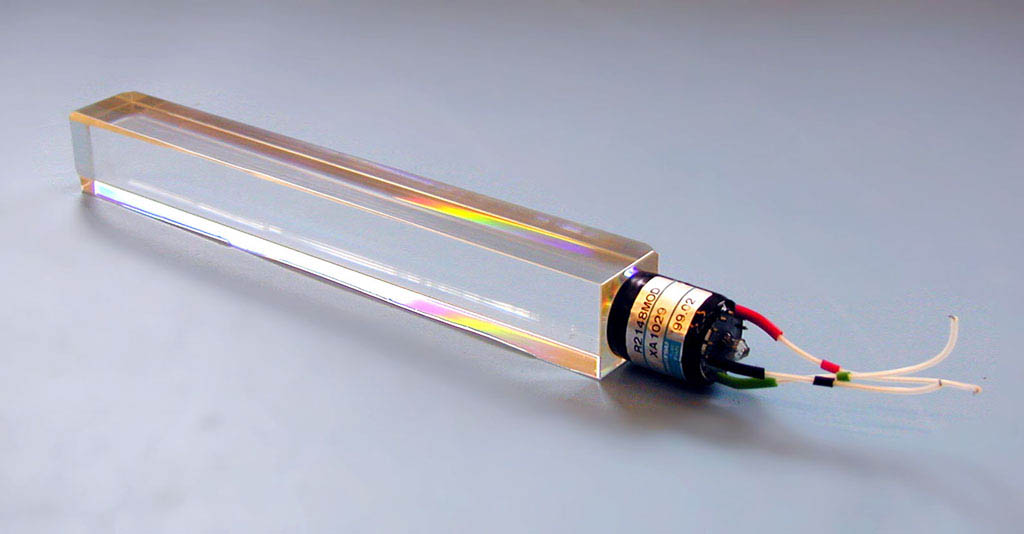
\includegraphics[width=0.7\textwidth]{Images/ECAL/Introduction/SC_VPT_and_crystal.jpg}    
    \caption{EE crystal with its attached VPT.}
    \label{fig:ECAL_XTAL}
\end{figure}
% \section{Trigger primitive generation} \label{sec:ECAL_TPG}

ECAL provides an input to the CMS Level-1 trigger in the form of trigger primitives. It is one of several inputs to the CMS Level-1 trigger, as shown in Figure \ref{fig:CMS_L1_Trigger}. This section is structured as follows: Section \ref{sec:ECAL_TP} will describe the composition of ECAL trigger primitives, and section \ref{sec:PU_Optimized_Weights} will describe a re-optimization of ECAL TP generation, known as PU optimized weights.  

\subsection{ECAL trigger primitives} \label{sec:ECAL_TP}

ECAL TPs are one of three inputs into the Layer 1 Calorimeter Trigger, shown in Figure \ref{fig:CMS_L1_Trigger}. The basic building blocks of ECAL TPs, with the Phase-I electronics used during LHC data-taking, are ``strips" composed of 5 crystals each in EB, and 1-5 crystals in EE. Every 25 ns, a digitized sample is taken of ECAL signals in every crystal, shown in Figure \ref{fig:ECAL_Waveform_Digis}. During data taking, this leads to a constant stream of values measured in ADC (analog to digital converter) counts. These values are linearized to account for different gains that may be set in different amplifiers, summed within a strip. For each set of 10 linearized strip samples, a digital filter made of a set of 10 FIR (Finite impulse response) weights is multiplied by their corresponding sample values and summed to obtain a transverse energy ($E_{T}$) value, shown in Equation \ref{eq:weights_equations}. In this equation, $S_{i}$ represents digitized sample ``i", where ``i" can range from 0-10 for the 10 digitized samples taken from an ECAL pulse from 0-225ns. Additionally, $w_{i}$ represents the FIR weight assigned to sample ``i", which is pre-determined for each ECAL strip. A requirement on the FIR weights is that they sum to zero, in order to include a dynamic pedestal subtraction, also shown in Equation \ref{eq:weights_equations}. This is performed for every subsequent set of 10 samples, with the window of 10 samples shifting 25ns forward each time, leading to a constant stream of $E_{T}$ values. Additionally, a peak finder is then applied to strip sums in order to determine which BX (Bunch crossing) in a predefined window of BXs has the greatest calculated $E_{T}$ value. Strip energies are then summed to form trigger towers (5 strips in EB, 1-5 strips in EE), for which TPs are formed. An ECAL TP is an $E_{T}$ value of a trigger tower at a given BX, with up to two feature bits. One feature bit is the fine grain bit, and is used to distinguish EM signals from jets. In EB TPs, a bit is also reserved for the rejection on anomalous signals termed ``spikes". When a BX has a TP created, the other BXs in the window are not eligible to have a TP formed. Non-zero TPs are sent to TCC (Trigger concentrator card) boards for further processing and time alignment before being sent to the L1 trigger. A schematic showing this process and computation of strip $E_{T}$ is shown in Figure \ref{fig:ECAL_TP_Formation}.

\begin{figure}[H]
    \centering
    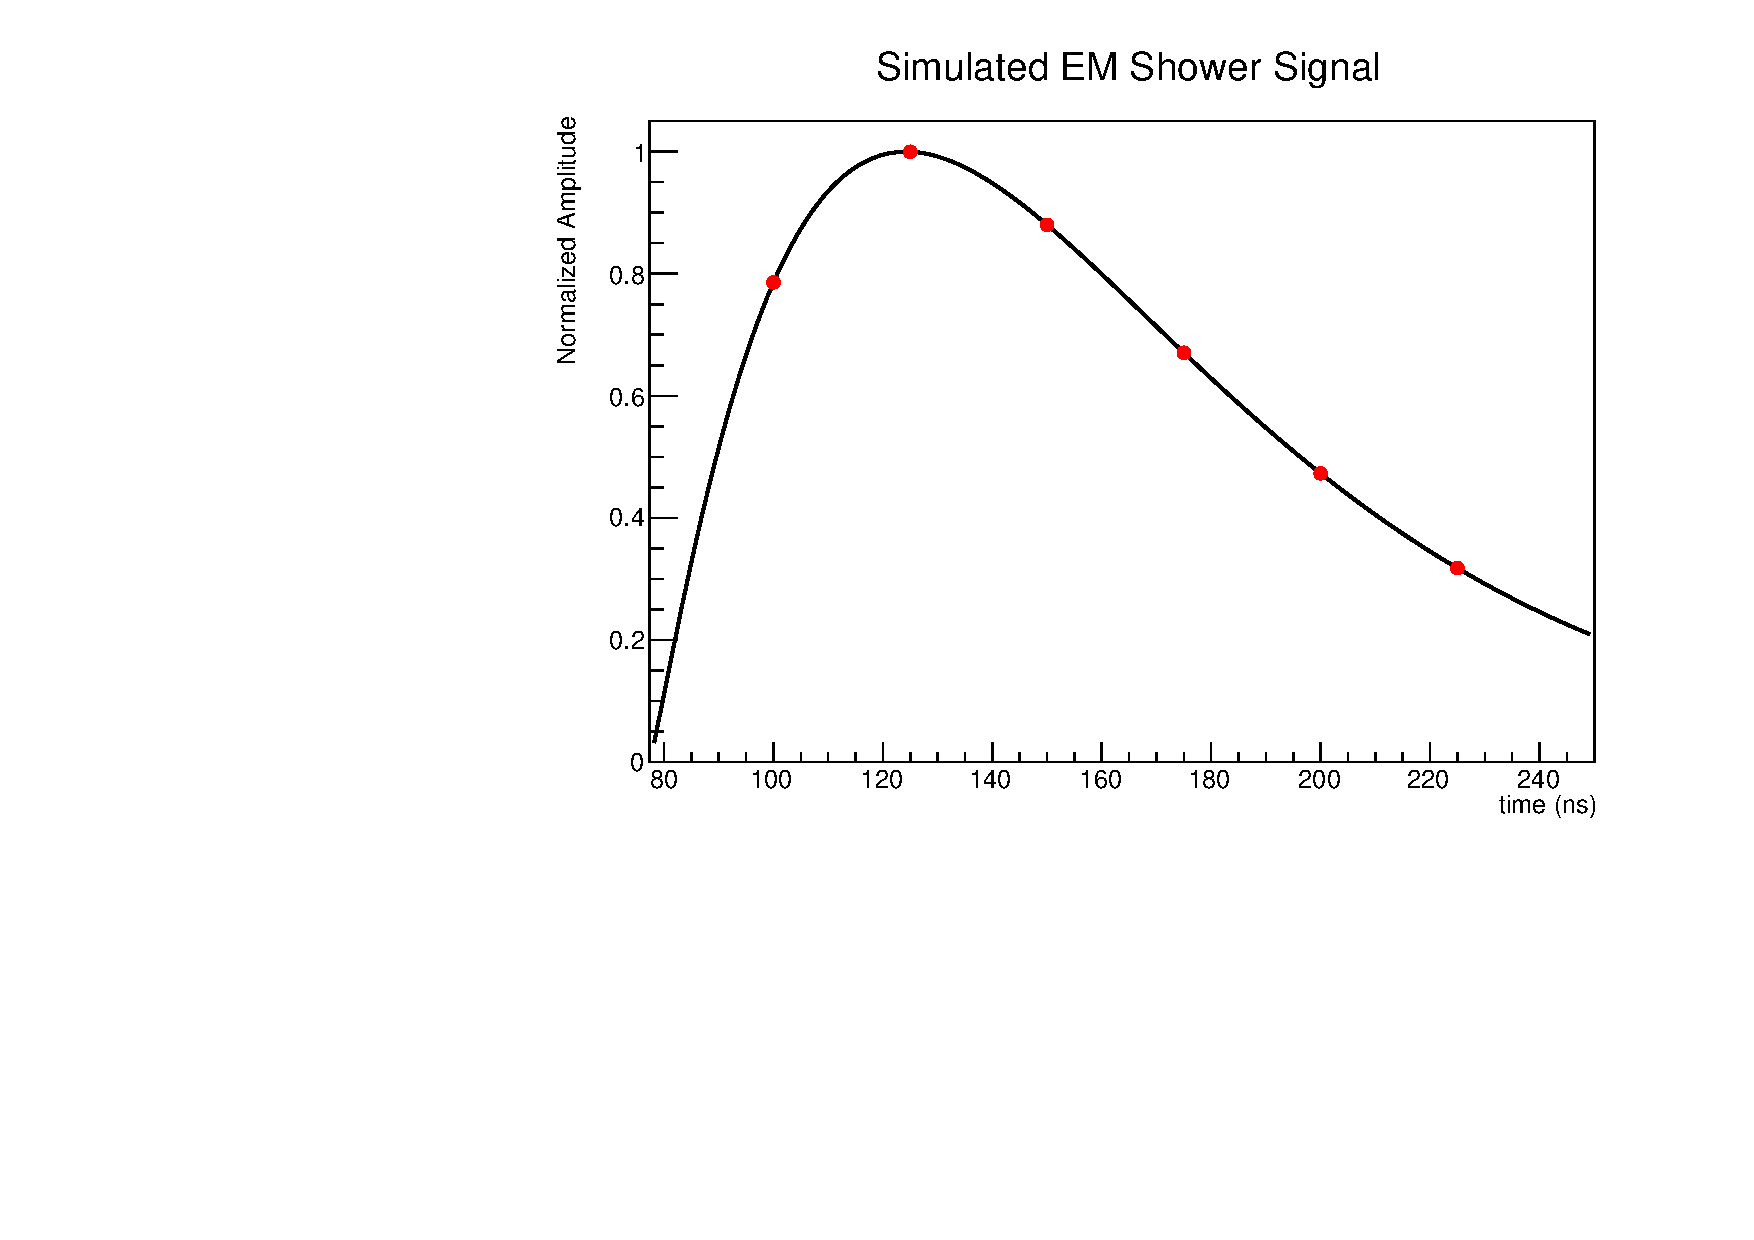
\includegraphics[scale=0.5]{Images/ECAL/TPG/EM_Waveform_Example.pdf}
    \caption{ECAL analog pulse shape example, with digitized samples taken every 25ns.}
    \label{fig:ECAL_Waveform_Digis}
\end{figure}

\begin{equation} \label{eq:weights_equations}
E_{T} = \sum_{i=1}^{10}S_{i}\times w_{i}
   \quad\text{,}\quad 
\sum_{i=1}^{10}w_{i} = 0 
\end{equation}

\begin{figure}[H]
    \centering
    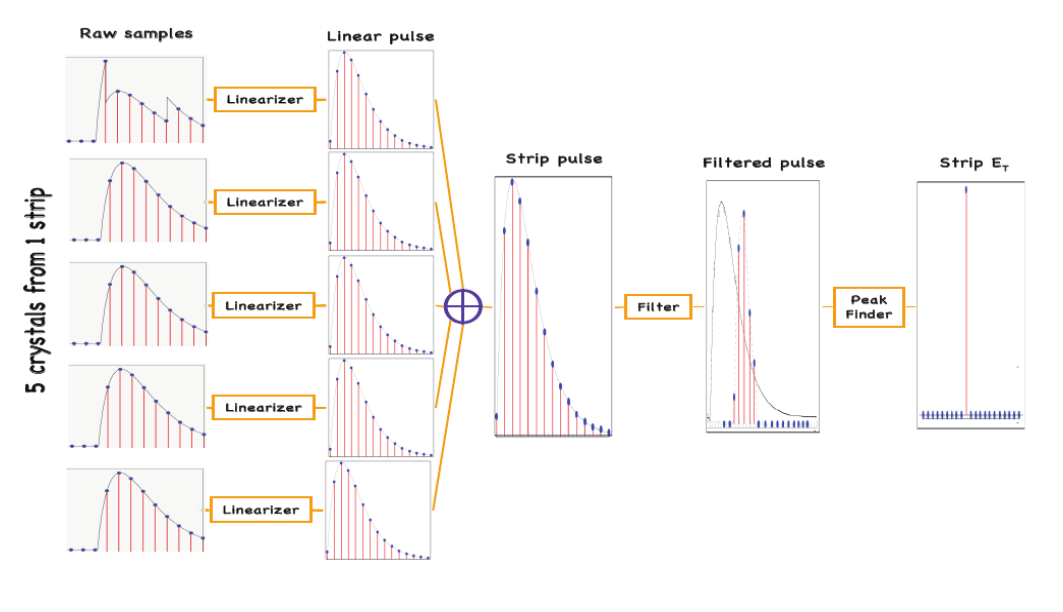
\includegraphics[width=\textwidth]{Images/ECAL/TPG/XTAL_To_ET.png} \caption{ECAL strip $E_{T}$ formation.}
    \label{fig:ECAL_TP_Formation}
\end{figure}

Each ECAL TP in EB and EE is composed of an $E_{T}$ value computed as the sum of its strip $E_{T}$ values, information bits, and a BX assignment. ECAL TPs are created on-detector, and are transmitted to the Level-1 trigger at the LHC collisions rate of 40 MHz. Because the transverse momentum of two LHC proton bunches before colliding is 0, the detection of hits with a high $E_{T}$ or \pt component is a potential sign of an interesting hard interaction between protons, and thus is a quintessential quantity to consider when forming an L1 decision.  

\subsection{PU optimized weights} \label{sec:PU_Optimized_Weights}

Throughout Runs 1 and 2, two sets of amplitude weights were used when computing ECAL strip energies and hence TP energies, one for EB and one for EE, shown in Figure \ref{fig:ECAL_weights}.

\begin{figure}[H]
\begin{center}
\begin{tabular}{ccccccccccc} \toprule

sample & 1 & 2 & 3 & 4 & 5 & 6 & 7 & 8 & 9 & 10 \\ \midrule
EB & 0 & 0 & -0.5625 & -0.546875 & 0.25 & 0.484375 & 0.375 & 0 & 0 & 0 \\ EE & 0 & 0 & -0.65625 & -0.515625 & 0.25 & 0.515625 & 0.40625 & 0 & 0 & 0 \\ \bottomrule

\end{tabular} 
\end{center}
\caption{Run 1 and 2 ECAL FIR weights} % \cite{DPG_Slides}
\label{fig:ECAL_weights}
\end{figure}

These FIR weight values were obtained from ECAL pulse shapes measured in test beams, as for a given waveform shape, an optimal set of weights can be extracted for measuring the waveform's height.

One way to simulate the photo-detectors' response to crystal scintillation is with an analytic waveform. The function used to simulate the time evolution of the detector response for each crystal is the alpha-beta function defined in Equation \ref{eq:alphaBetaFunction}. 

\begin{equation} \label{eq:alphaBetaFunction}
	f(t) = 	
	\begin{cases} 
      f(t) = A*\Bigg(1 + \dfrac{(t - t_{0})}{(\alpha\beta)}\Bigg)^{\alpha}*e^{\frac{-(t-t_{0})}{\beta}} & t > (t_{0} - \alpha*\beta) \\
     0 & t \leq (t_{0} -\alpha*\beta)
  \end{cases}
\end{equation}

In this equation, A is the height of the waveform in ADC counts, $t_{0}$ is the time of the waveform's peak in nanoseconds, $\alpha$ describes the behavior of the polynomial term, and $\beta$ corresponds to the decay time in the exponential term. The pedestal (P) can also be set, giving the full analytic form of the detector response shown in Equation \ref{eq:FullECALresponsefcn}.

\begin{equation} \label{eq:FullECALresponsefcn}
G(t;P) = f(t)+P
\end{equation}

With dedicated fine grain time scans performed on ECAL signals, the parameters $A$, $t_{0}$, $\alpha$ and $\beta$ were measured for each crystal during Run 2. These scans were performed in October 2017, June 2018, and September 2018, and a variation of the parameters among the crystals can be seen over time due to the ageing of ECAL crystals caused by steady dosages of radiation from LHC collisions. 

By producing and sampling these waveforms and applying the Run 2 FIR weights to the samples, one can simulate the reconstructed amplitude of the ECAL TPs as a function of pseudorapidity ($\eta$). A fractional amplitude bias, defined as the percent difference between the reconstructed amplitude, $\hat{A}$ and the true amplitude $A$ and shown in Equation \ref{eq:bias}, is shown as a function of $\eta$ in Figure \ref{fig:ampBiasvseta} \cite{CMS-DP-2019-031, CMS-DP-2019-031_Plots}. 

\begin{equation} \label{eq:bias}
    \text{bias} = \frac{\hat{A}}{A} - 1
\end{equation}

\begin{figure}[H]
    \centering
    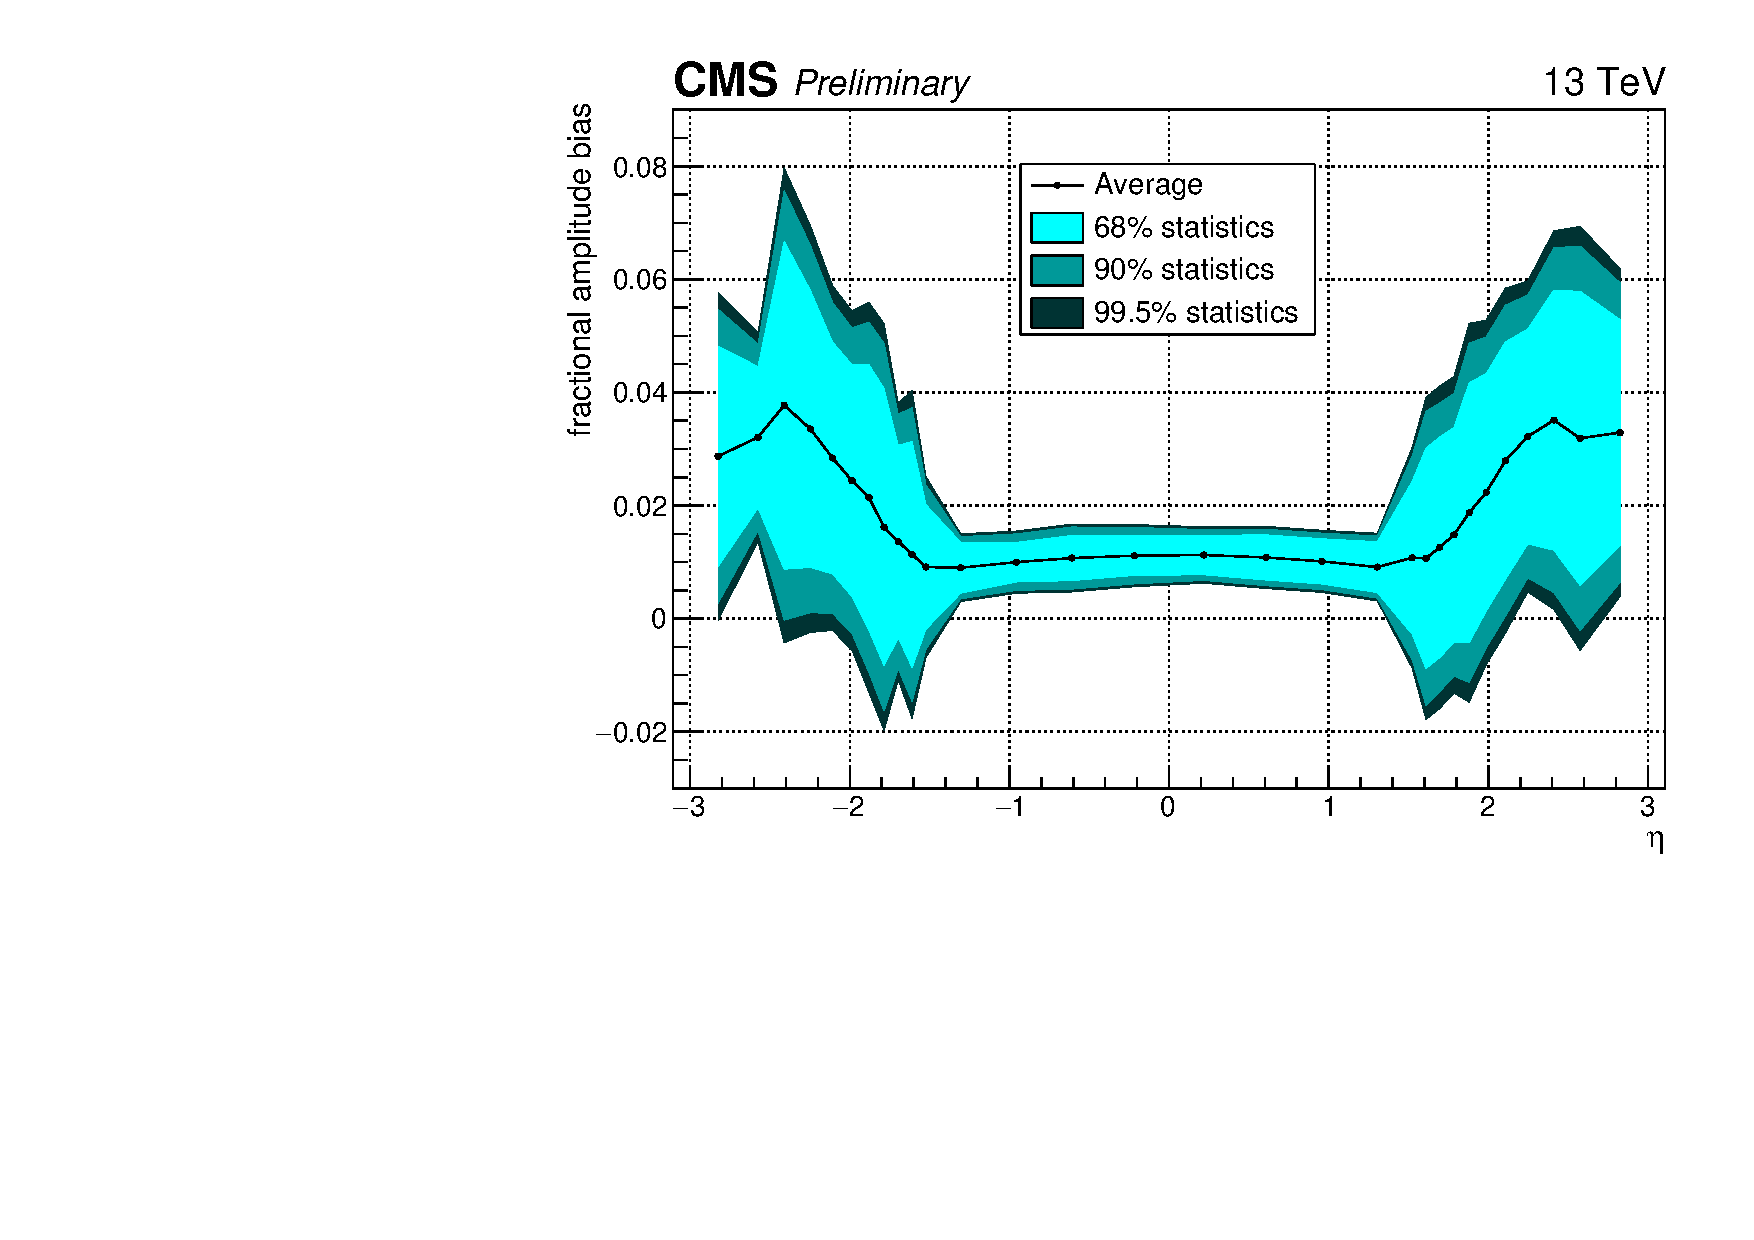
\includegraphics[width=\textwidth]{Images/ECAL/TPG/AmpBias_vs_eta_Sep18_ps.pdf}
    \caption{Average bias vs. $\eta$, with no simulated time shift (ts = 0ns), using September 2018 parameters for detector response and Run 2 weights for reconstruction.}
    \label{fig:ampBiasvseta}
\end{figure}

It can be seen from this result that there is a bias in the reconstructed amplitude, particularly in the high-$\eta$ region where a greater average and spread of bias is present. In the high-$\eta$ region occupied by the EE, the average fractional amplitude bias is about a factor of three larger than that in the EB region. This is consistent with the fact that ECAL crystals in the high-$\eta$ region receive more radiation from LHC collisions, and therefore their crystals and corresponding waveforms are more distorted and stray further from their original shapes use to derive their FIR weights. This indicates that a more ideal set of weights can be produced in order to produce more accurate TPs. This motivates the derivation of new amplitude weights to see if a reduction in bias average and spread can be made. 

In order to derive updated amplitude weights, a simulation of ECAL electronics' response to scintillation light was setup from the most recent timing scan data obtained in September 2018, including a realistic PU scenario which depends on $\eta$, and distorts the in-time ECAL pulses. Using the alpha-beta analytic waveform to model each crystal's response, and taking a realistic PU energy spectrum and LHC proton bunch train into account (48b7e), the fractional spread of energy biases was computed as a function of signal BX shown in Figure \ref{fig:gr_train_nonzero_Asf_48b7e_0_8_std} for ECAL EB crystals with $|\eta| < 0.7$, and for EE crystals with $2.3 < |\eta| < 3.0$ in Figure \ref{fig:gr_train_nonzero_Asf_48b7e_26_28_std} \cite{CMS-DP-2022-016, CMS-DP-2022-016_Plots}

\begin{figure}[H]
    \centering
    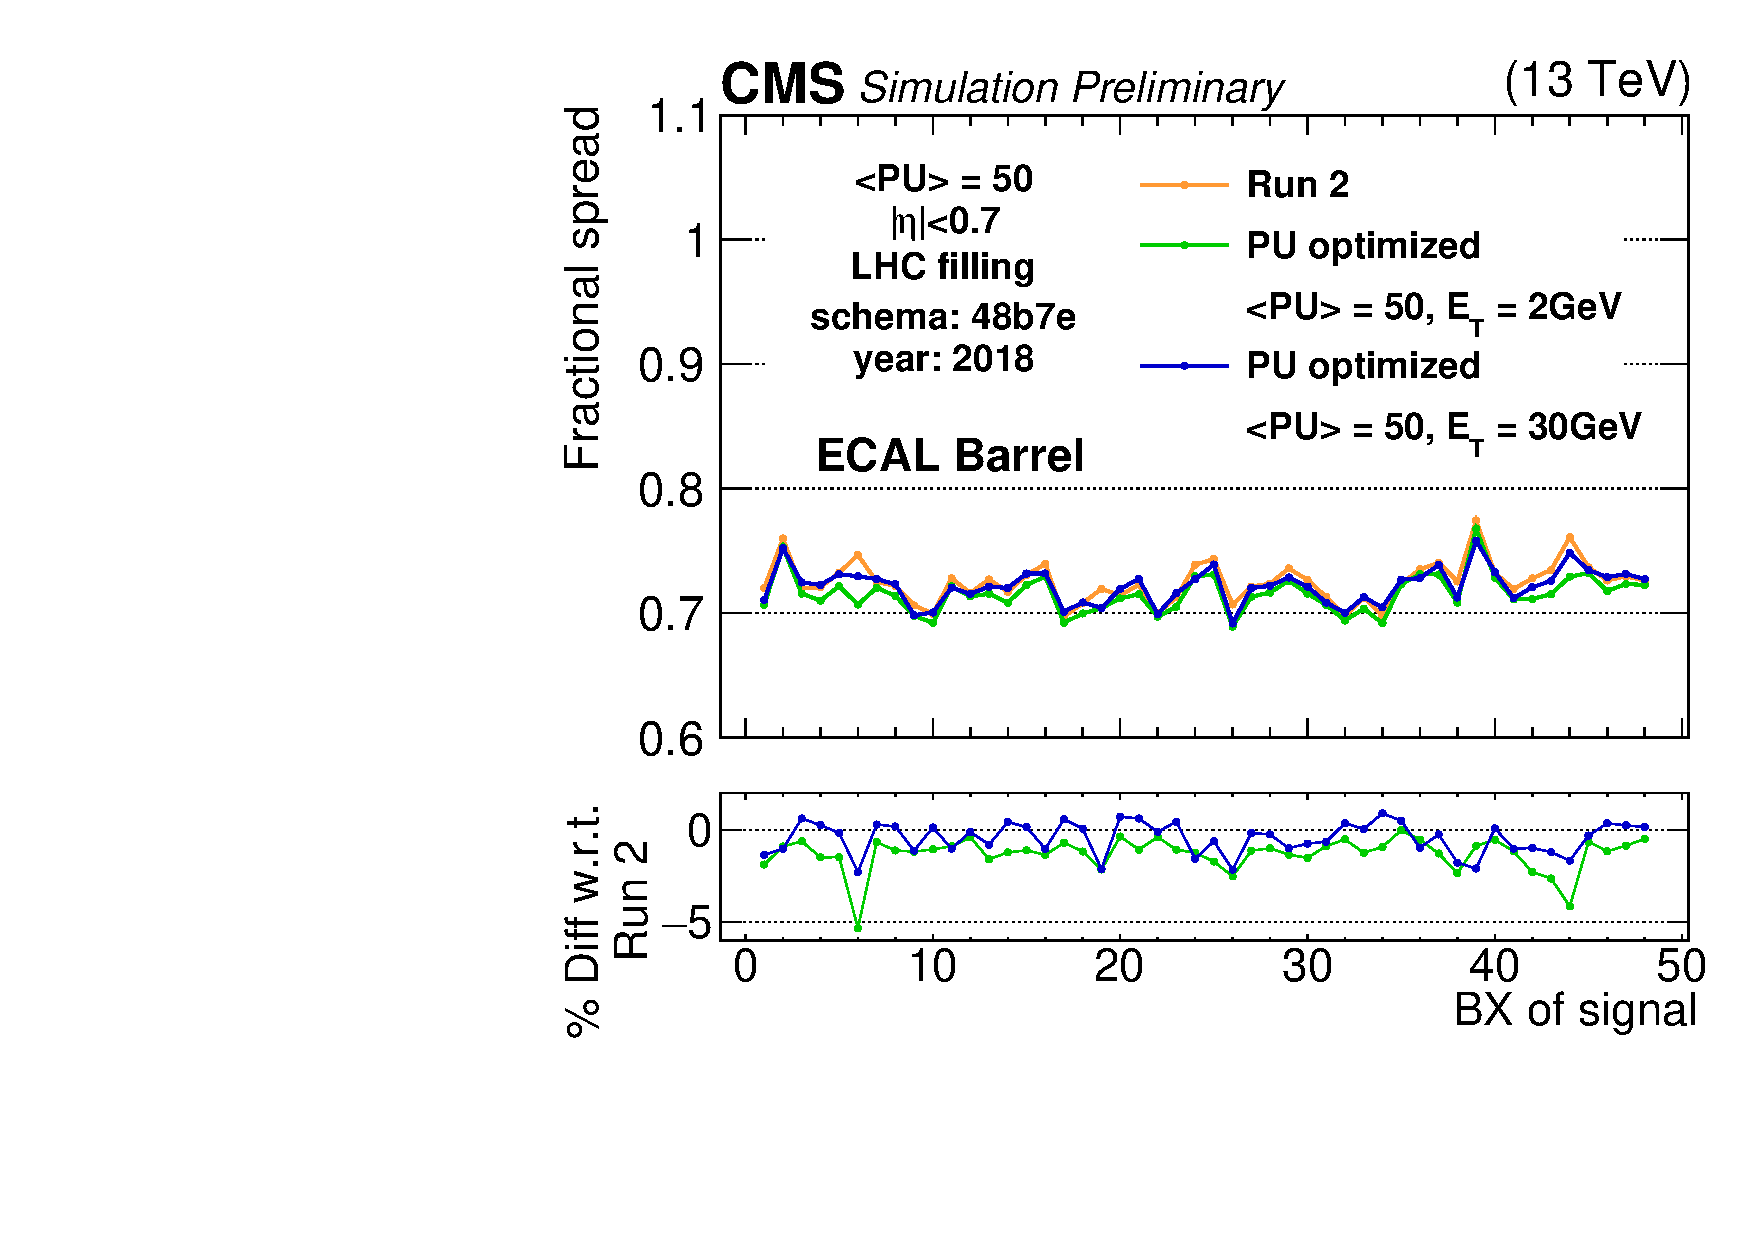
\includegraphics[width=\textwidth]{Images/ECAL/TPG/gr_train_nonzero_Asf_48b7e_0_8_std.pdf}
    \caption{Fractional spread of amplitude bias for simulated ECAL crystal responses in the region $|\eta| < 0.7$.}
    \label{fig:gr_train_nonzero_Asf_48b7e_0_8_std}
\end{figure}

\begin{figure}[H]
    \centering
    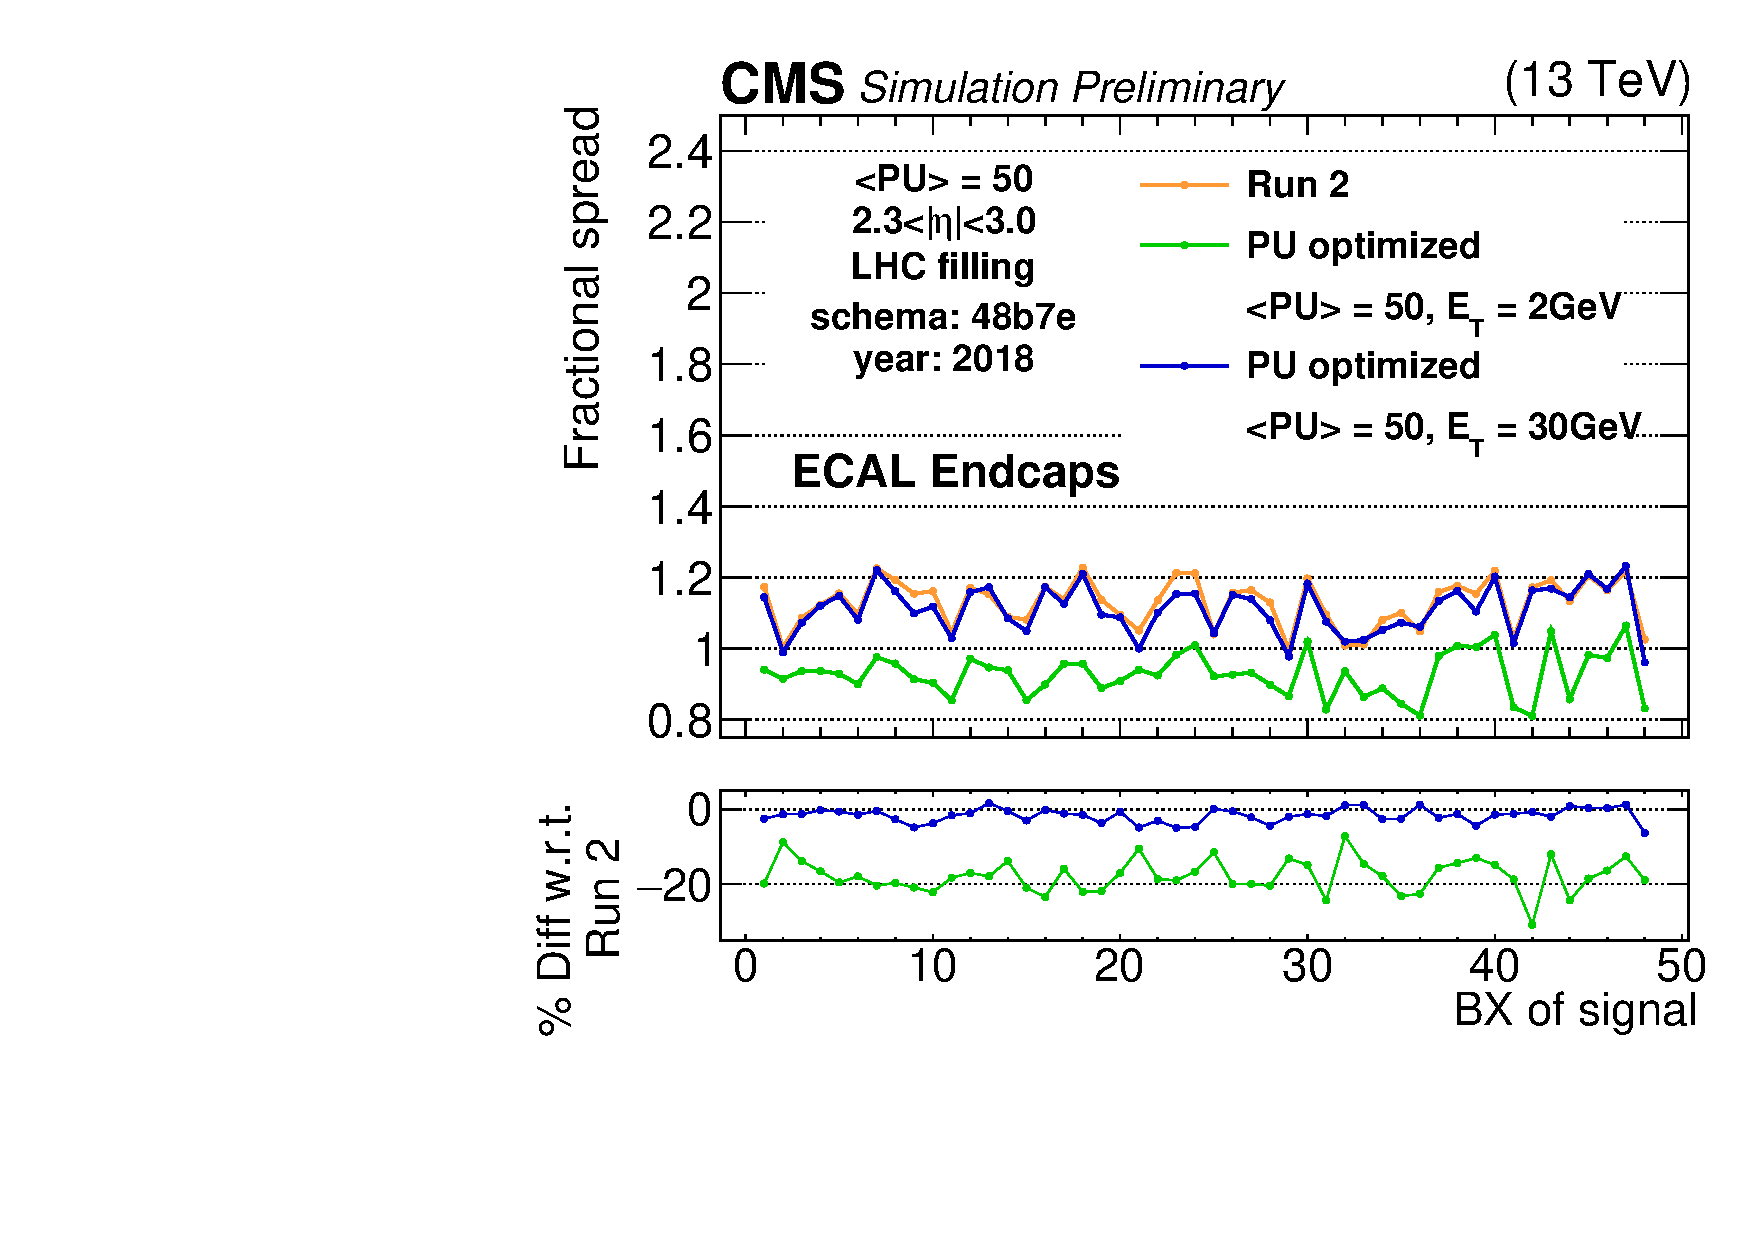
\includegraphics[width=\textwidth]{Images/ECAL/TPG/gr_train_nonzero_Asf_48b7e_26_28_std.pdf}
    \caption{Fractional spread of amplitude bias for simulated ECAL crystal responses in the region $2.3 < |\eta| < 3.0$.}
    \label{fig:gr_train_nonzero_Asf_48b7e_26_28_std}
\end{figure}

For both ECAL regions, fractional spread is shown when reconstructing amplitude with the Run 2 weights, PU optimized weights optimized for a strip $E_{T}$ of 2 GeV, and for a strip $E_{T}$ of 30 GeV. In the EB region, an improvement in fractional spread of about 1\% is obtained with respect to Run 2 weights when using weights optimized for PU and $E_{T}$ = 2 GeV. In EE, a more drastic improvement of about 15-20\% is obtained with respect to Run 2 weights. This is consistent with Figure \ref{fig:ampBiasvseta}, which shows there is more room for improvement in EE compared to EB. 

This indicates that updating the existing EB and EE FIR weights may improve the spread of fractional bias in TP $E_{T}$ computation. The effect of updated ECAL TP FIR weights on Level-1 quantities, and further evaluation of the potential gain from updating the ECAL L1 amplitude weights to account for changes in ECAL pulse shapes due to ageing and PU is currently being studied and tested in an effort to improve ECAL for Run 3. A potential positive impact of improved ECAL TP resolution is an increase in the L1 tagging efficiency of electron and photon objects, which can potentially increase the efficiency of triggering on HH$\rightarrow$WW$\gamma\gamma$ events, and events with similar signatures, at the CMS detector. 

In addition to amplitude weights, sets of timing sensitive weights can also be derived. Instead of returning an amplitude when multiplied by waveform samples, these return timing jitter, defined as the time displacement from the expected peak time. These ideal sets of weights are derived to return a bias of 0 when the input waveform is the one they were derived from. Therefore, the effectiveness of these two types of weights can be shown by plotting their bias when different time shifts are applied, defined as a translation of the waveform left or right. For example, a time shift of 5 ns means $t_{0}$ would go from $t_{0}$ to $t_{0} + 5ns$. The average fractional amplitude and time biases as a function of time shift are shown in Figures \ref{fig:ampBiasvsTimeShift} and \ref{fig:timeBiasvsTimeShift}. 

\begin{figure}[H]%
    \centering
    \subfloat[Average amplitude bias vs. time shift \label{fig:ampBiasvsTimeShift}]{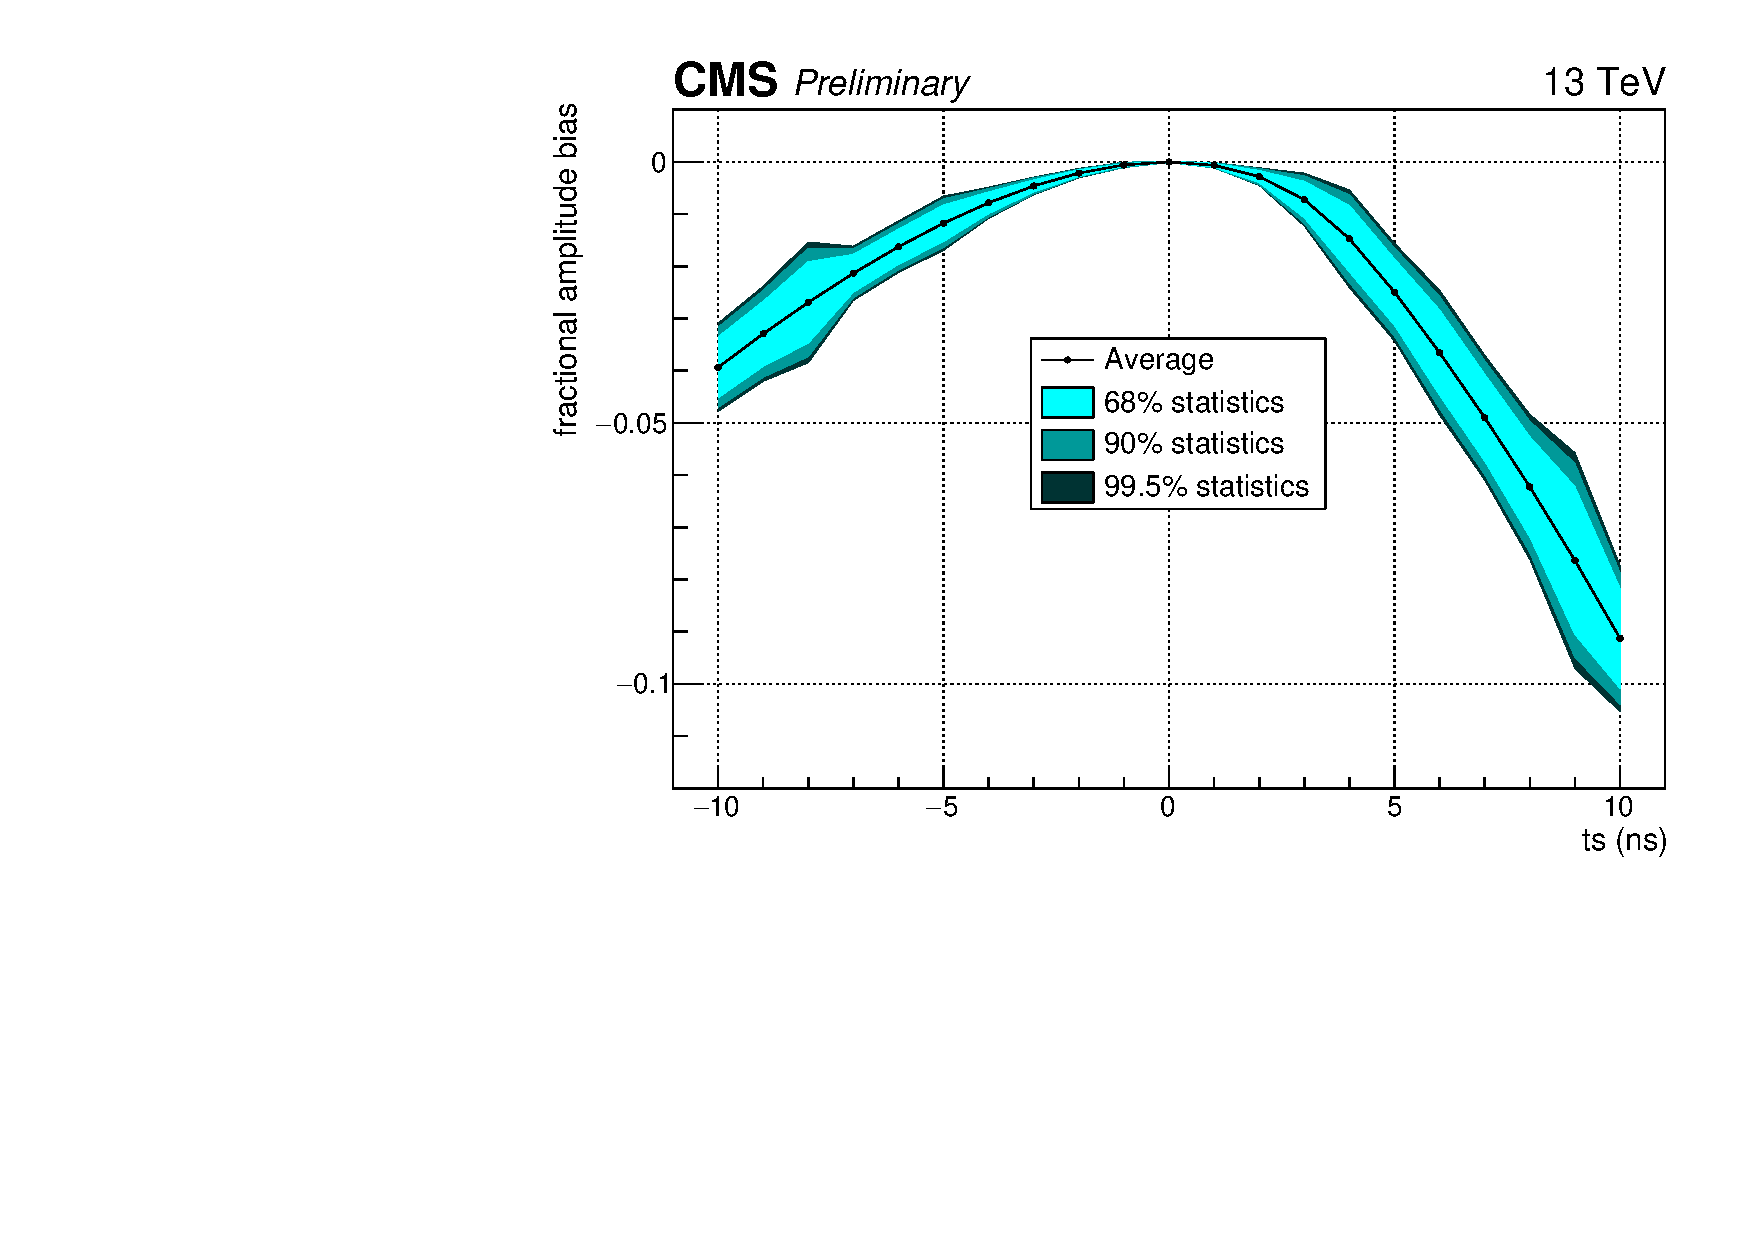
\includegraphics[width=0.8\textwidth]{Images/ECAL/TPG/AmpBias_vs_ts_Sep18_Id.pdf}}%
    \\ \newline 
    \subfloat[Average timing bias vs. time shift \label{fig:timeBiasvsTimeShift}]{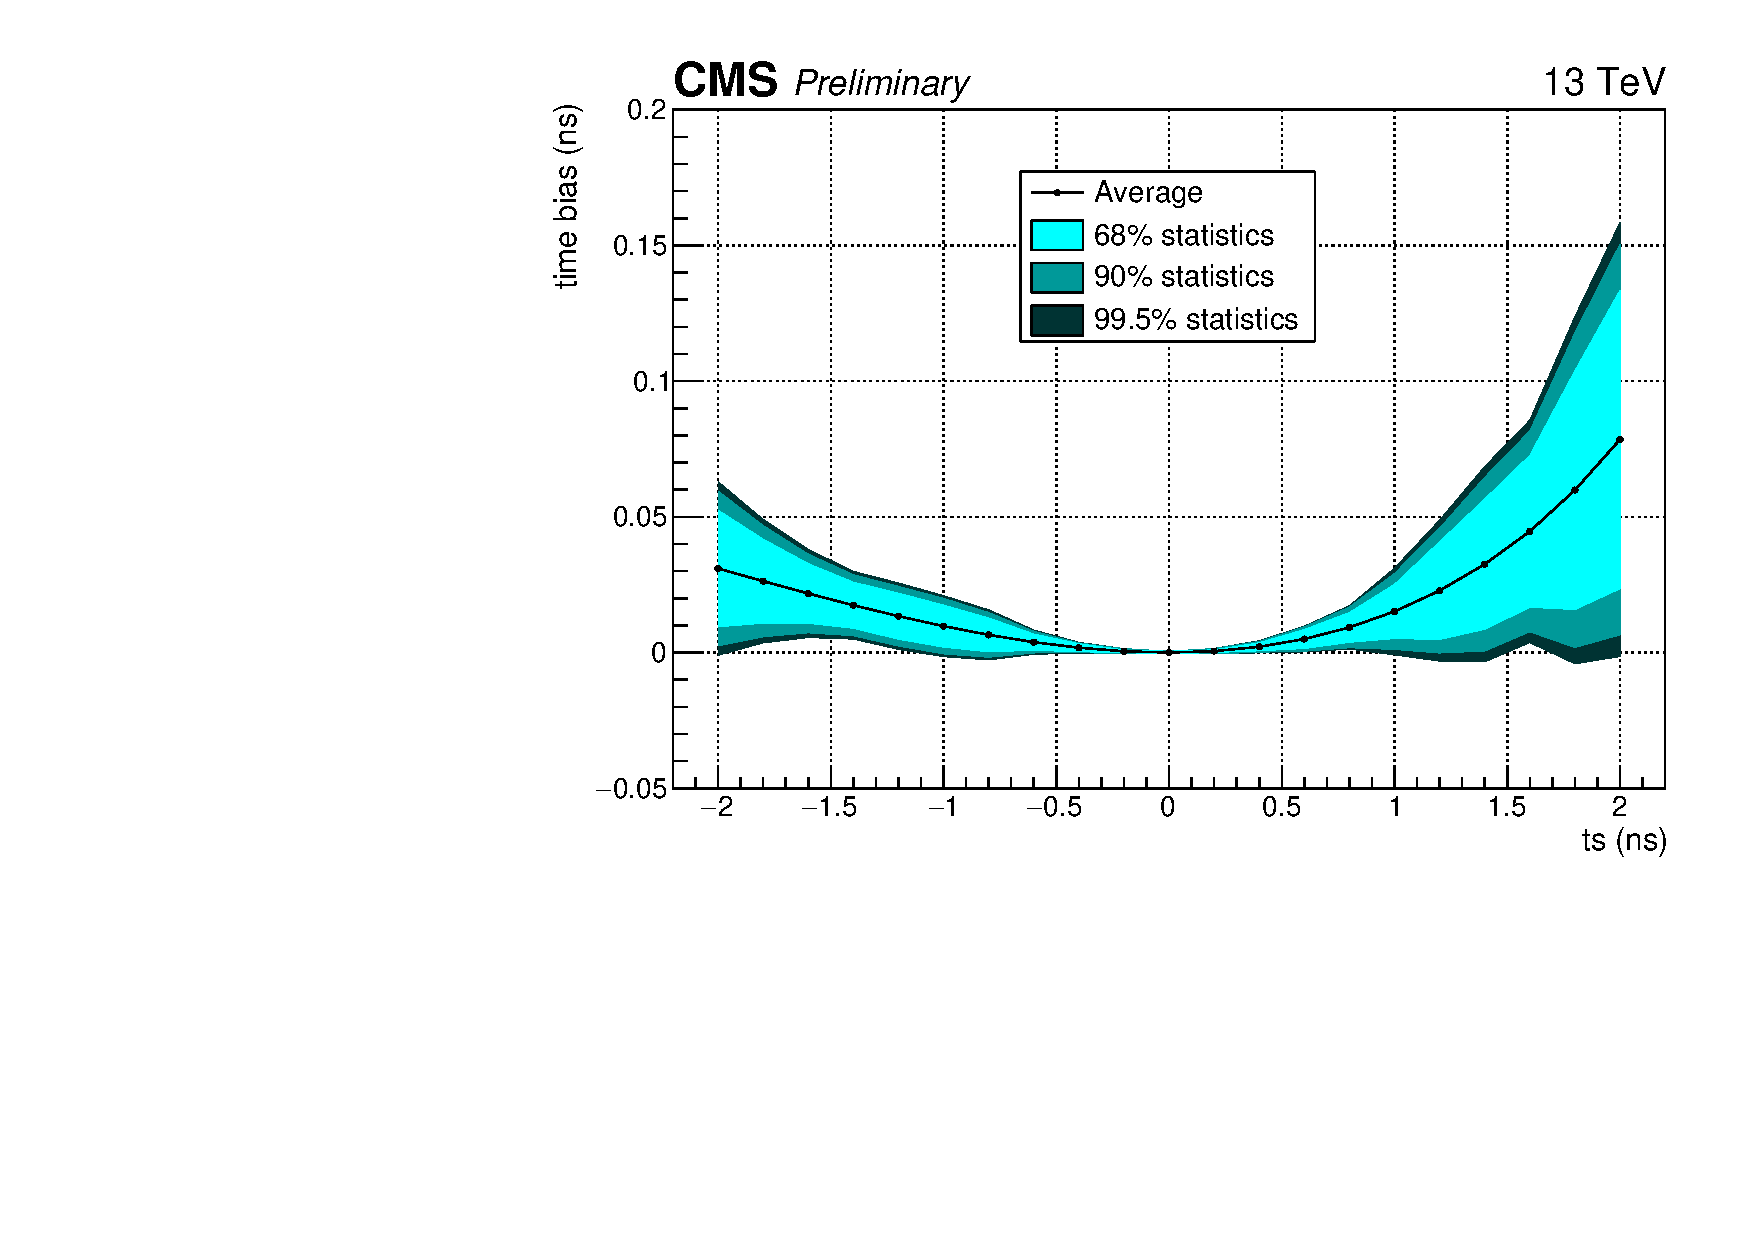
\includegraphics[width=0.8\textwidth]{Images/ECAL/TPG/TimeBias_vs_ts_Sep18_Id.pdf}}%
    \caption{(a) Amplitude and (b) time bias vs time shift for ECAL waveforms, using September 2018 parameters for detector response and ideal weights for reconstruction, for crystals in the $\eta$ region: $(-3.0,-2.6)$}%
\end{figure}

For time shifts of 0, there is no bias in amplitude or timing weights because the weights were derived for each non-time-shifted waveform. Because the bias is not large for small time shifts, ideal weights can be considered worth investigating. 

\section{Double weights} \label{sec:DW}

Throughout LHC Runs 1 and 2, the on-detector ECAL FENIX chip, a custom ASIC, was used for energy reconstruction to form $E_{T}$ sums for ECAL TPs, multiplying one set of weights by recorded digis as described in Section \ref{sec:ECAL_TP}. During LS2, it was discovered that the ECAL FENIX chip has the capacity to store and use two sets of weights. This essentially duplicates the ECAL FENIX data path, as shown in Figure \ref{fig:DW_Diagram}, into two electronically equivalent paths, one for each FIR filter named the ``EVEN" and ``ODD" filters.

\begin{figure}[H]
    \centering
    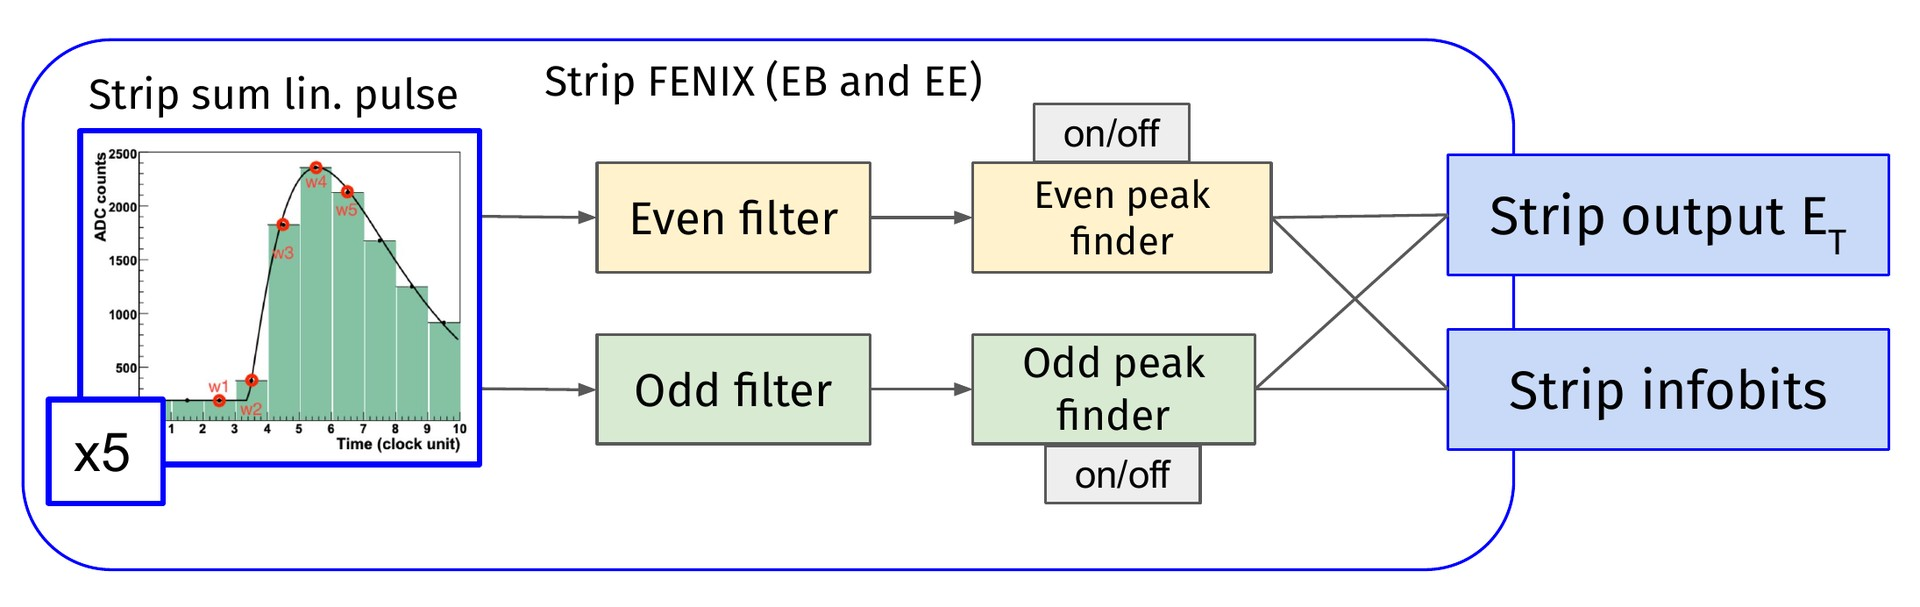
\includegraphics[width=\textwidth]{Images/ECAL/DW/ECAL_DW_Schematic.png}
    \caption{ECAL double weights mechanism.}
    \label{fig:DW_Diagram}
\end{figure}

This feature was implemented in the ECAL FENIX chip for potential further use, but was never used during Runs 1 and 2. 

\subsection{Spikes} \label{sec:spikes}

A commonly observed phenomenon at the ECAL is the direct ionization of the ECAL EB APDs, which produce anomalous signals termed ``spikes". Because these signals do not come from electromagnetic showers originating from the hard interactions of LHC collisions, they must be removed as efficiently as possible to keep trigger rates under control and preserve the quality of the offline reconstruction of electrons, photons and jets. Additionally, spike progenitors often spend time propagating in the CMS detector before directly ionizing the EB APDs, and therefore may be out-of-time with respect to electromagnetic signals.

There is a method in place used to remove spikes at L1 using a topological cut, termed the ``spike killer" \cite{Petyt_2012}. This operates by making a topological cut, exploiting the fact that spikes typically deposit all of their energy into a single ECAL crystal as they are due to the direct ionization of APDs, while EM showers are expected to be spread among multiple crystals. A diagram showing the mechanism of the spike killer is shown in Figure \ref{fig:spikeKillerDiagram}. 

\begin{figure}[H]
    \centering
    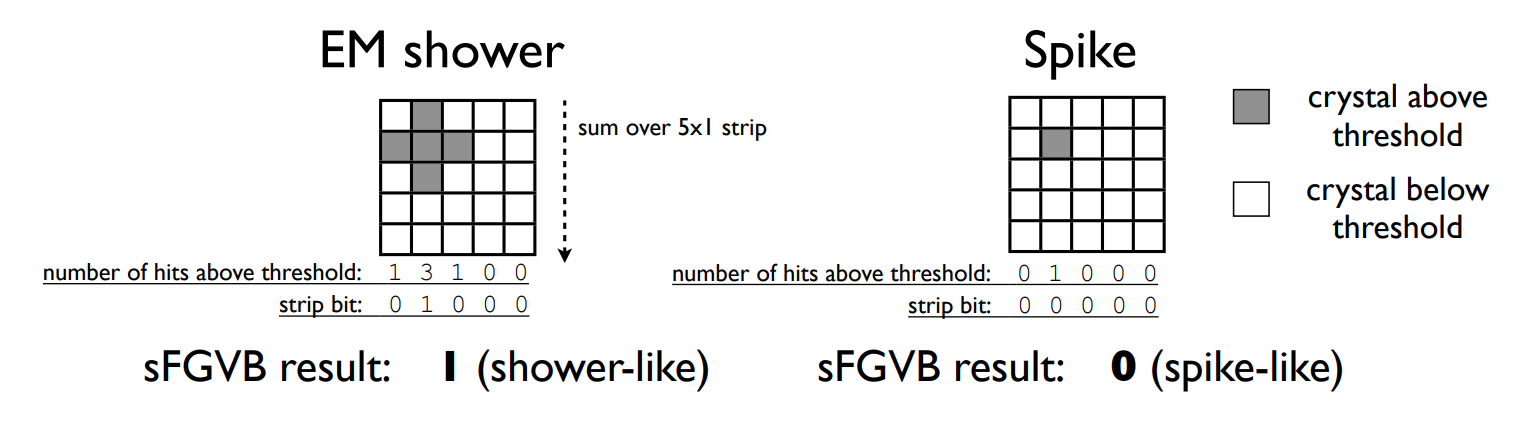
\includegraphics[width=\textwidth]{Images/ECAL/DW/SpikeKillerDiagram.png}
    \caption{Operation of the strip Fine-Grained Veto Bit (sFGVB) on an electromagnetic shower (left) and a spike-like energy deposit (right).}
    \label{fig:spikeKillerDiagram}
\end{figure}

The spike killer makes use of a per-strip bit, the strip Fine-Grained Veto Bit (sFGVB) which is set to 1 if at least 2 crystals in a strip are above a per-crystal energy threshold. If a trigger tower (set of 25 crystals, 5 strips) has at least one strip with a sFGVB equal to 1, it is preserved as it is considered EM shower-like due to its spread in energy. However, if a TT has no strips with at least one sFGVB set to 1, the TP energy is set to 0 if its energy is above the spike killer ``killing threshold" of 16 GeV. 

In order to optimize the spike killer for Run 3 where higher noise and everage PU is expected, the per-crystal energy threshold was increased, as there will be a higher expected contribution from noise and PU for all crystals. The spike contamination among TPs with the Run 2, and candidate Run 3 working point is shown in Figure \ref{fig:spikeKillerRun3optimization}. Notably in this spike contamination plot, produced using data from a ZeroBias dataset (no triggering on typical physics menus), there is a high spike contamination at high energy. This is because it is more likely to produce a high energy spike, which are high energy due to its direct ionization of the APDs, than a high energy EM shower, which requires the production of a truly high energy particle from proton-proton interactions. 

\begin{figure}[H]
    \centering
    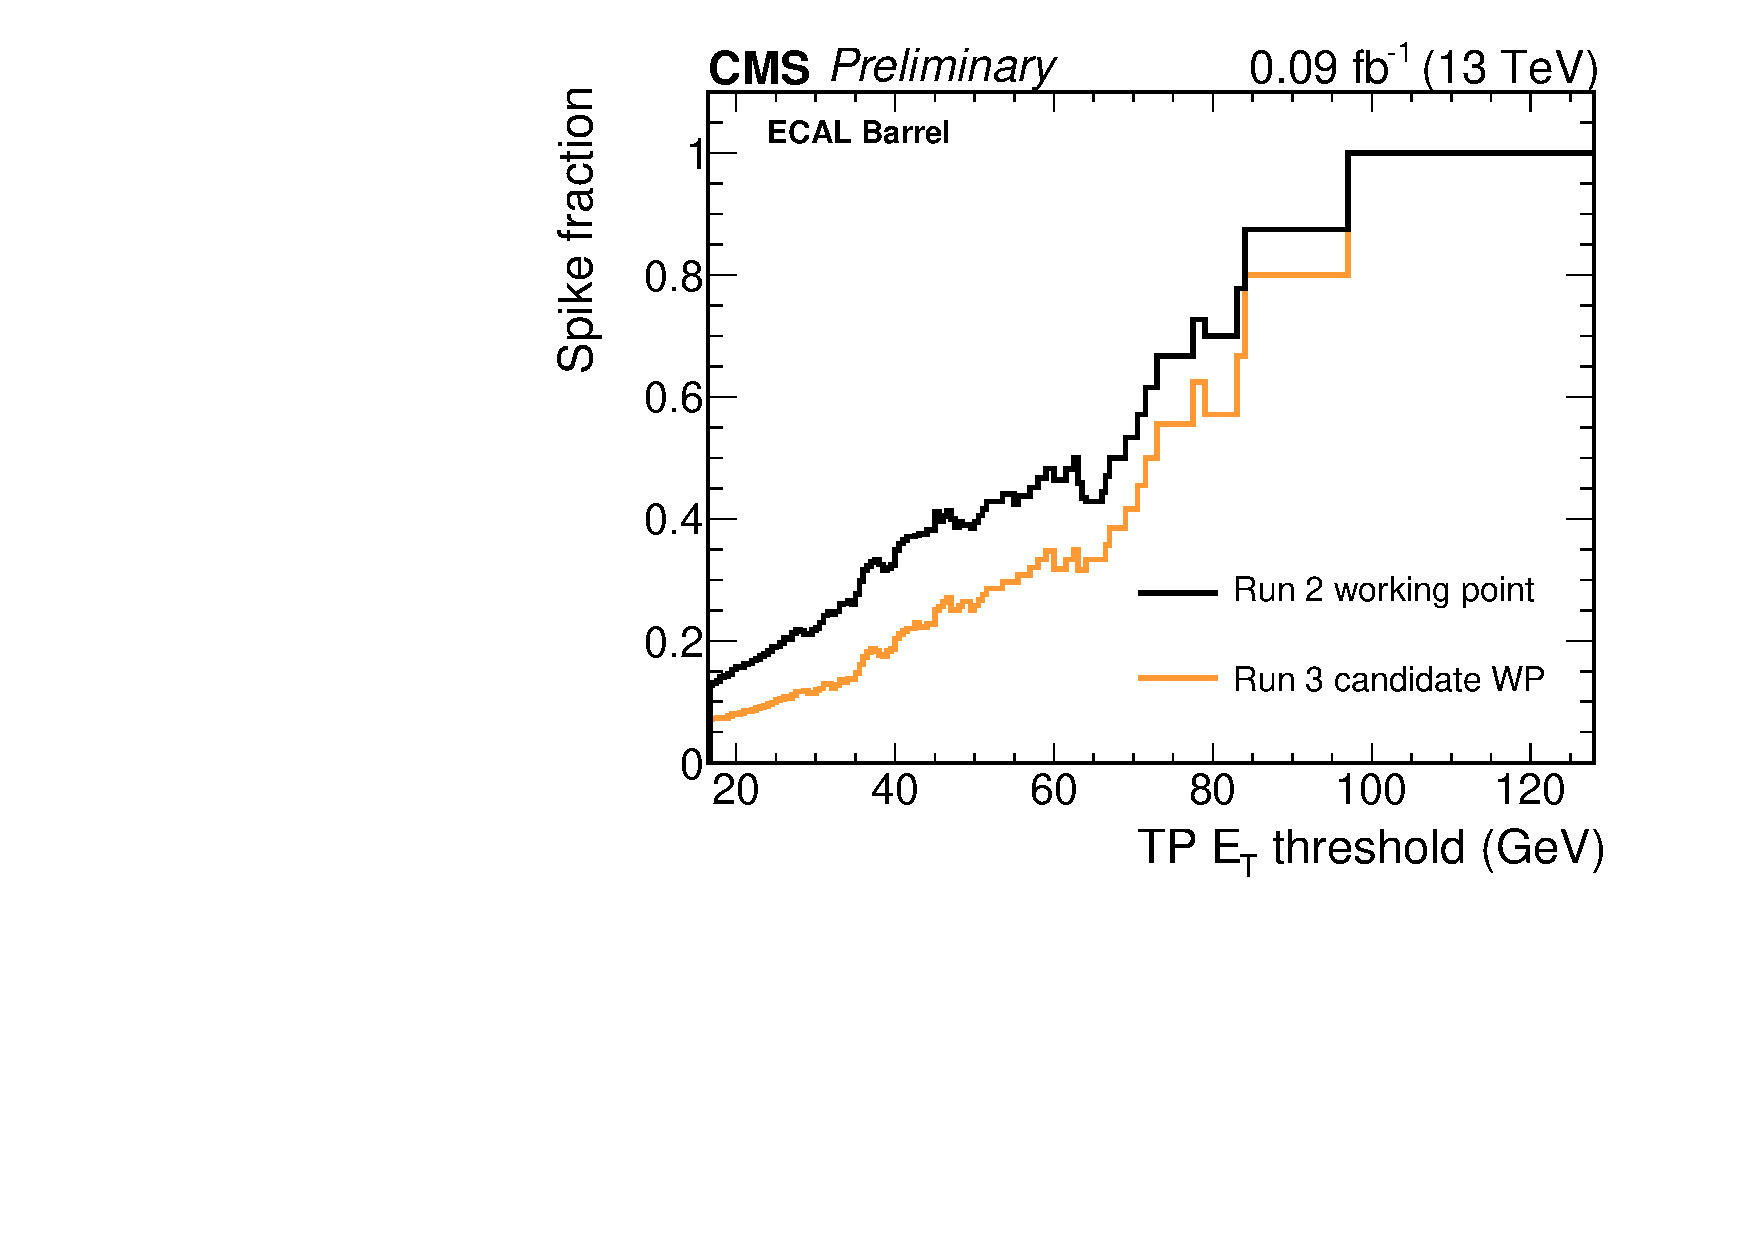
\includegraphics[width=0.8\textwidth]{Images/ECAL/DW/spikekiller_run3_optimisation.pdf}
    \caption{Spike fraction vs. TP $E_{T}$ threshold with a Run 2, and Run 3 candidate working point of the existing ECAL L1 spike killer. The data comes from a ZeroBias dataset recorded in July 2018 with a peak pileup of 50.}
    \label{fig:spikeKillerRun3optimization}
\end{figure}

This shows that while updating the settings of the existing spike killer to a candidate Run 3 working point removes additional spikes at Level-1, there is much room for improvement, especially in the high energy regime. Additionally, at L1 there is no existing spike killer in the low energy regime 0-16 GeV, as this is below the spike killer threshold. 

\subsection{Timing weights}

The initial idea for optimizing ECAL double weights was to keep the original set of amplitude weights in the EVEN filter, and to utilize the second set of weights, the ODD filter, as a set of timing weights in order to compute an on-detector timing value for trigger primitives. These studies showed possible discrimination power, as the timing weights were able to identify out of time signals which came from spikes. Figures \ref{fig:ampvstime_EMlike} and \ref{fig:ampvstime_Spikelike} show the reconstructed amplitude computed as the EVEN weights times signal digis, vs. the reconstructed time as computed by multiplying a set of optimal timing weights occupying the ODD filter by signal digis for signal and spike-like TPs in CMS data. 

\begin{figure}[H]
    \centering
    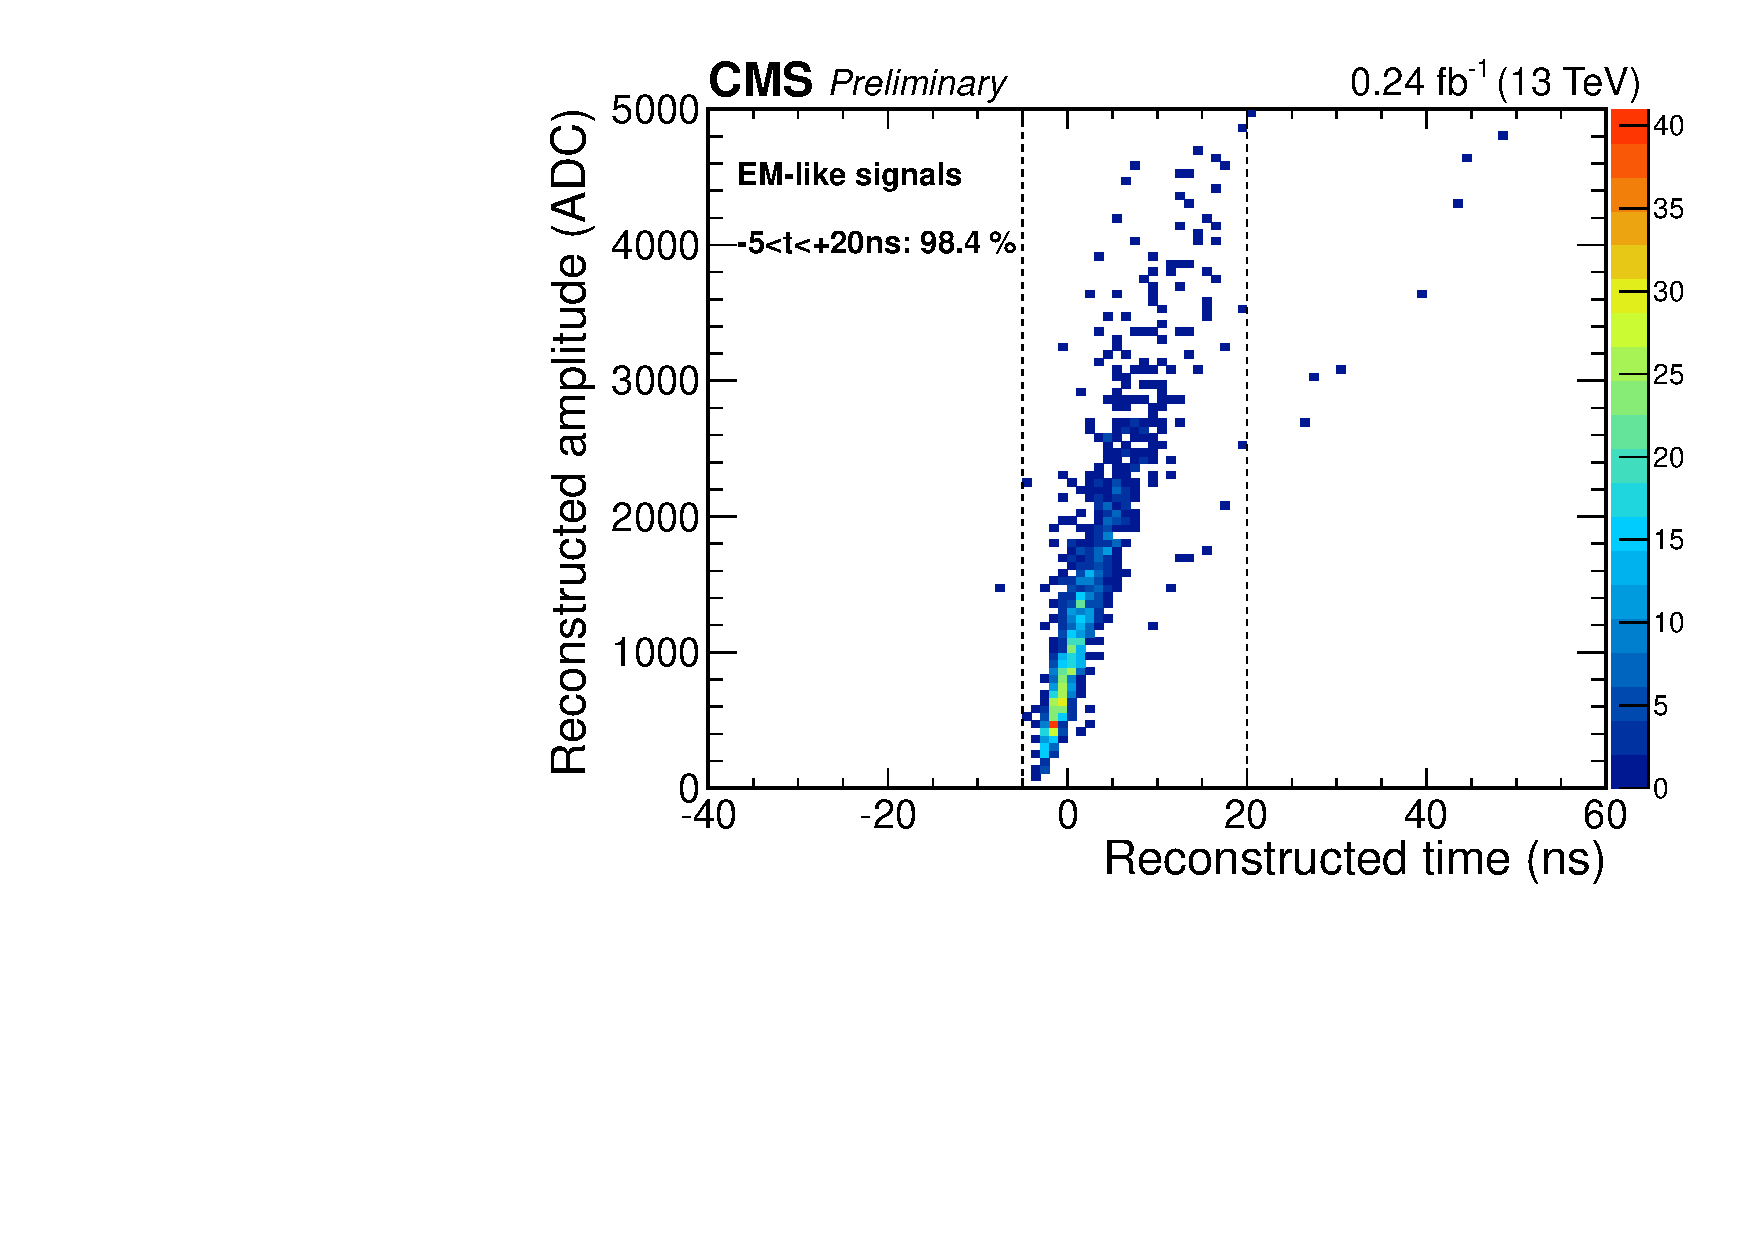
\includegraphics[width=0.8\textwidth]{Images/ECAL/DW/EM_TPs.pdf}
    \caption{Reco amplitude vs. Reco time of EM-like signals in CMS data}
    \label{fig:ampvstime_EMlike}
\end{figure}

\begin{figure}[H]
    \centering
    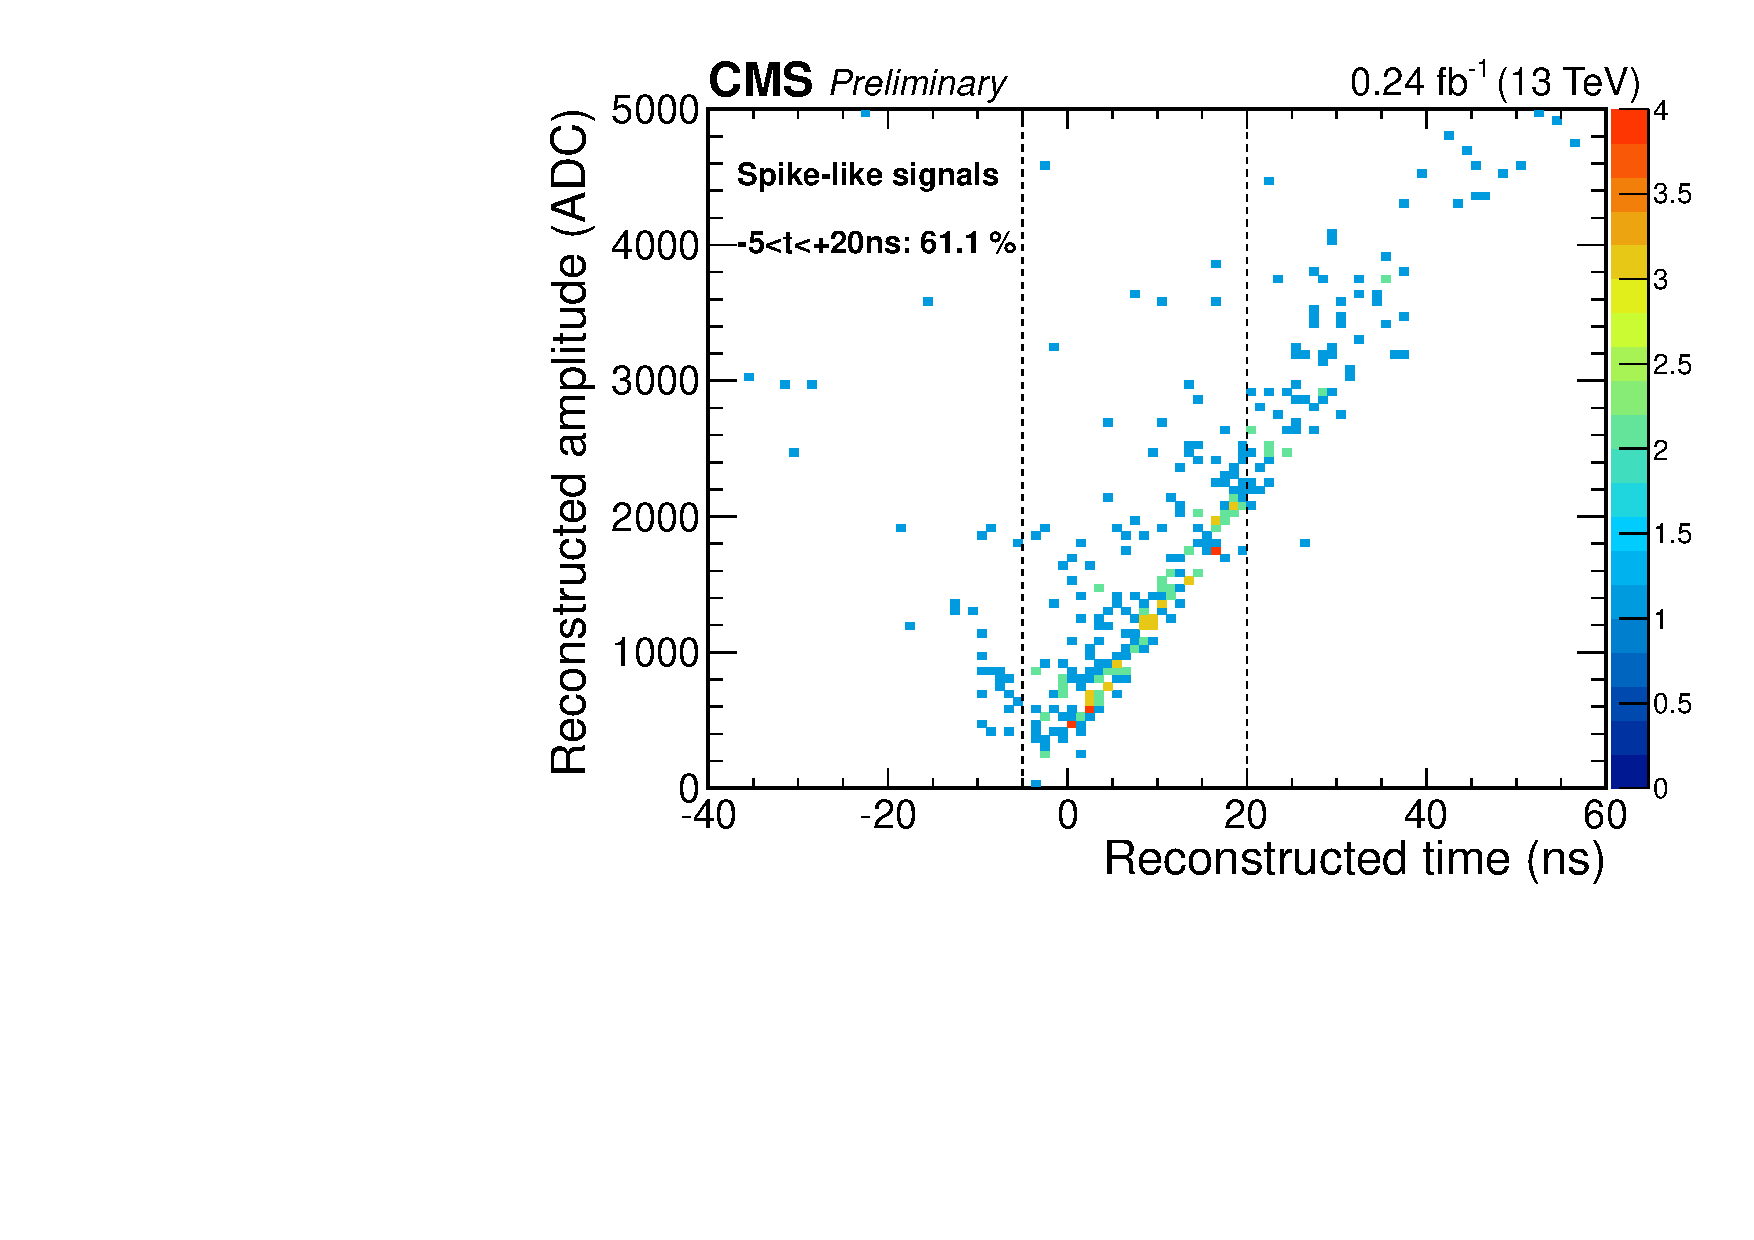
\includegraphics[width=0.8\textwidth]{Images/ECAL/DW/Spike_TPs.pdf}
    \caption{Reco amplitude vs. Reco time of spike-like signals in CMS data}
    \label{fig:ampvstime_Spikelike}
\end{figure}

By eye, most EM-like signals fall within a reconstructed time window near zero, with a tail going out to around 20 ns for signals with a greater reconstructed amplitude. For spike-like signals, there is a larger time window with some TPs very out-of-time. Interestingly, in the EM-like signals on Figure \ref{fig:ampvstime_EMlike} one can see a low population line of entries which appears to follow the trend of the spike-like signals in Figure \ref{fig:ampvstime_Spikelike}, as these are possibly real spikes which are incorrectly tagged offline as signal-like. 

For the sake of quantifying the possible discrimination power of ECAL timing weights, a hypothetical timing cut of -5 $<$ t $<$ 20 ns would have been able to drastically reduce the rate of spikes, as shown in Figure \ref{fig:TimingCutSpikeReduction}.

\begin{figure}[H]%
    \setcounter{subfigure}{0} % reset subcaption counter to 0 (a) 
    \centering
    \subfloat[Spike Rates]{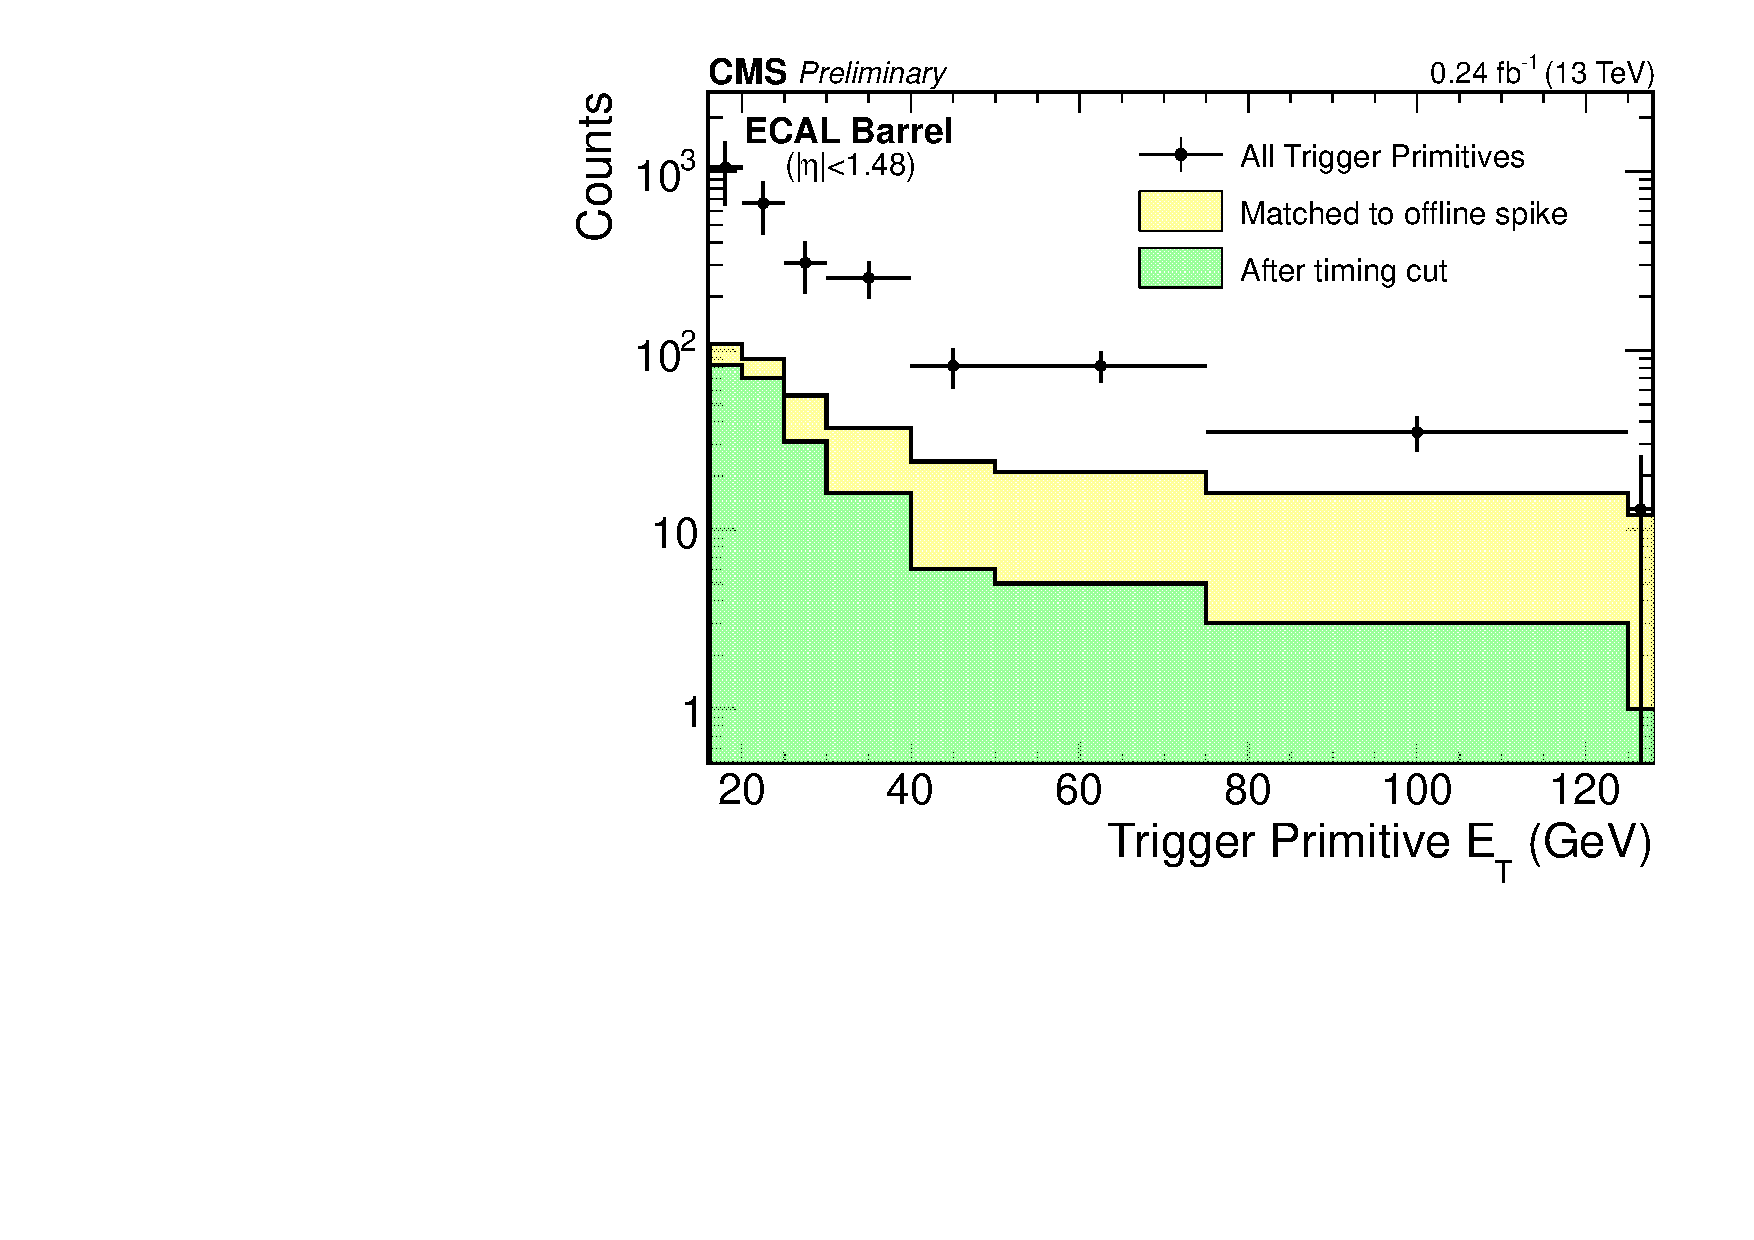
\includegraphics[width=0.49\textwidth]{Images/ECAL/DW/spikeTPet_beforeaftertimingcut.pdf}}%
    %\qquad
    \subfloat[Spike Fractions]{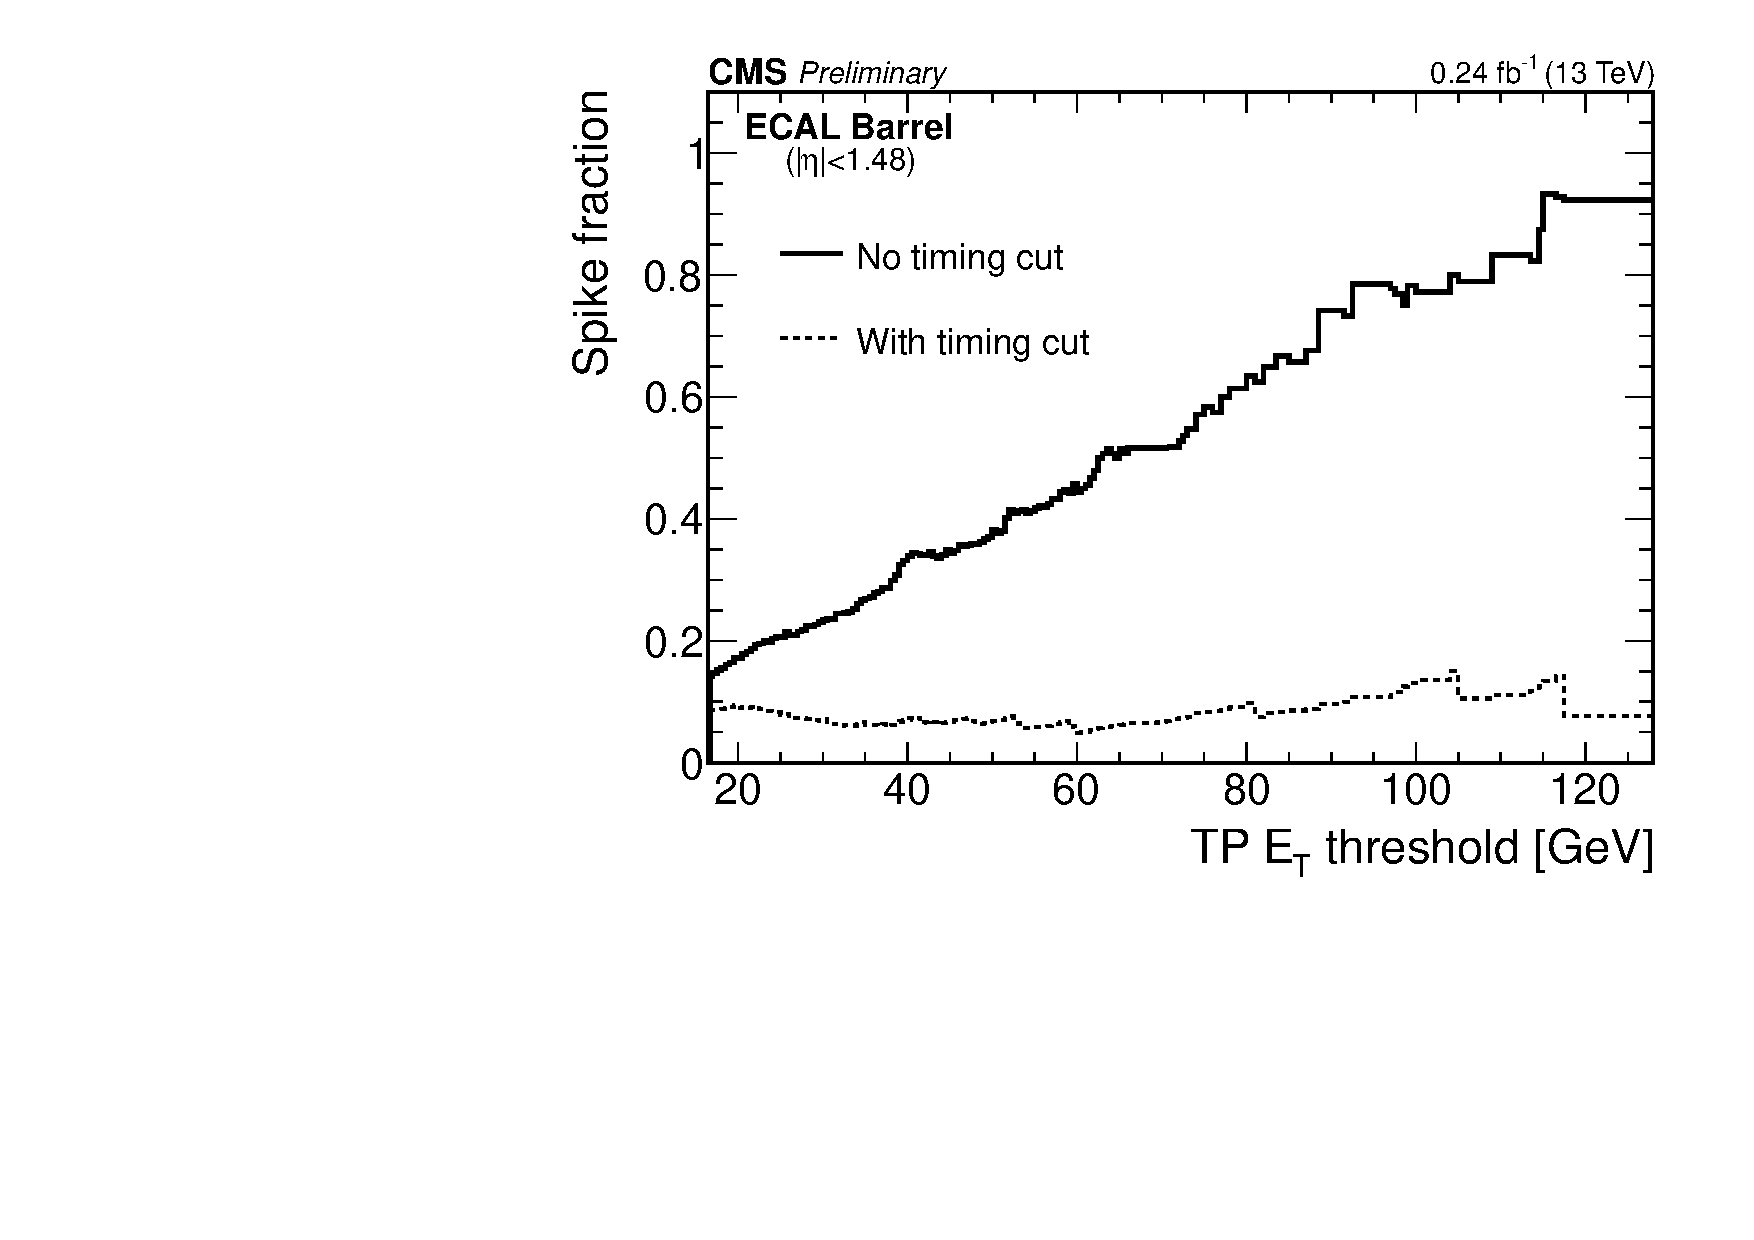
\includegraphics[width=0.49\textwidth]{Images/ECAL/DW/spikecontamination_beforeaftertimingcut.pdf}}%
    \caption{Spike quantities with/without timing cut \href{https://twiki.cern.ch/twiki/bin/view/CMSPublic/EcalDPGResultsCMSDPS2019031}{[EcalDPGResults]},\href{https://cds.cern.ch/record/2690933/files/DP2019_031.pdf}{[CDS]}}%
    \label{fig:TimingCutSpikeReduction}
\end{figure}     

A timing cut like this is not possible in the ECAL FENIX chip; However this study motivated the idea to use two sets of amplitude weights and a comparator in the FENIX chip in order to identify out-of-time signals with double weights. 

\subsection{Optimization}

In the ECAL FENIX chip, it is possible to compute two amplitudes via two sets of weights, and utilize a comparator in the electronics to set a boolean flag if one amplitude output is greater than the other. If an ODD set of weights is optimized to identify out of time signals, it is expected to returns a greater amplitude for out-of-time signals than the Run 2 weights designed for in-time signals. Therefore, the approach is taken to optimize an ODD set of weights for out-of-time signals.

Choosing an odd set of weights for out-of-time signal tagging is a multivariate problem, which must consider a realistic signal energy spectrum, spike energy spectrum, spike timing PDF, and the effects of pileup on signal waveform distortion. Therefore in order to extract ODD weights sets which are optimized to maximize signal efficiency and spike rejection, a numerical optimization was setup in order to derive optimal sets of weights to take the place of the second FIR filter weights. This optimization makes use of simulated signal waveforms using the alpha-beta analytic representation and simulated pileup described in Section \ref{sec:PU_Optimized_Weights}, and the simulation of spike waveforms from a standalone simulation. The optimization is setup as a loss minimization problem which makes use of gradient descent computation and backwards propagation of loss to maximize the amount of spike rejection, while minimizing the amount of signal rejection. This is incorporated in a loss definition, shown in Figure \ref{fig:NumOptLoss}.

\begin{figure}[H]%
    \setcounter{subfigure}{0} % reset subcaption counter to 0 (a) 
    \centering
    \subfloat[Loss function]{
\includegraphics[width=0.31\textwidth]{Images/ECAL/DW/LossFunction.png}}%
    \hfill
    \subfloat[Use of $\delta_{min}$ in loss]{
\includegraphics[width=0.31\textwidth]{Images/ECAL/DW/deltamin_use.png}}%
    \hfill
    \subfloat[Definition of ODD weights loss limit.]{
\includegraphics[width=0.31\textwidth]{Images/ECAL/DW/W2LossLimit.png}}
    \caption{Loss definition used in optimization of ODD set of amplitude weights.}%
    \label{fig:NumOptLoss}
\end{figure}  

One of the input parameters in the optimization is a minimum separation of the two amplitude values computed by the EVEN (default weights) and ODD (out-of-time sensitive) sets of weights, termed $\delta_{min}$. Varying this parameter results in different working points. The different portions of a simulated spike timing PDF which were tagged as out of time by different working points is shown in Figure \ref{fig:DW_StandaloneSimulation_SpikeTimingPDFTagging} \cite{CMS-DP-2022-007, CMS-DP-2022-007_Plots}. 

\begin{figure}[H]
    \centering
    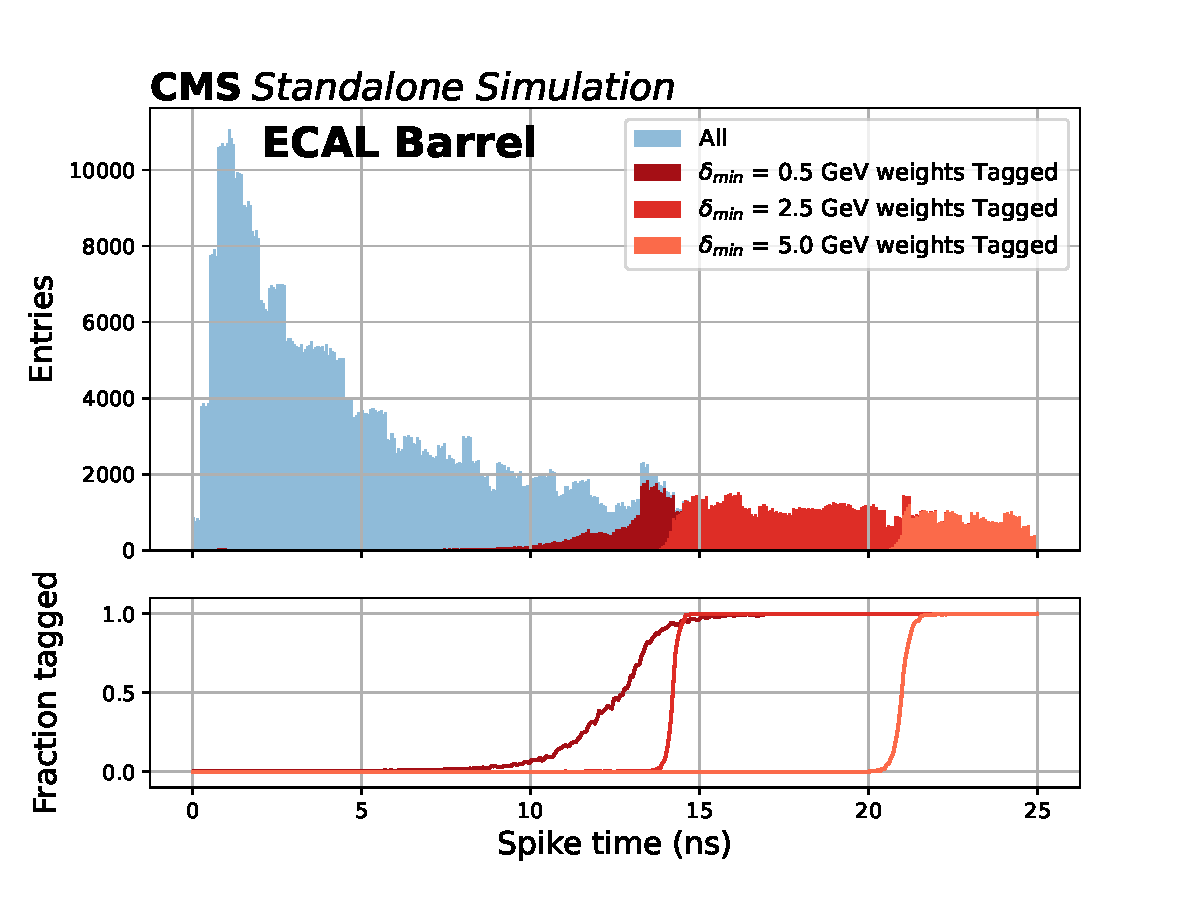
\includegraphics[width=0.8\textwidth]{Images/ECAL/DW/Double_Amplitude_Weights_SpikeTaggingwithOOTWeights_allDeltaMins.pdf}
    \caption{Tagging of out of time spikes in a standalone simulation.}
    \label{fig:DW_StandaloneSimulation_SpikeTimingPDFTagging} 
\end{figure}

In the spike timing PDF, most spikes are relatively in-time with respect to EM signals, while a non-negligible fraction have a late out of time tail. The reason for this is because spike progenitors often spend time propagating in the CMS detector before directly ionizing the EB APDs. It can be seen that increasing the value of the $\delta_{min}$ parameter tags later out of time spikes. This is somewhat expected, as a larger $\delta_{min}$ value will only use spike examples with larger differences in EVEN and ODD amplitudes in its optimization, which is more likely to come from out-of-time shifted spikes. 

While quantifying the expected gain in spike rejection from different $\delta_{min}$ working points, it is also important to check their effect on EM shower-like signals, as shown for a standalone simulation in Figure \ref{fig:SimSignaltaggedvsE}. 

\begin{figure}[H]
    \centering
    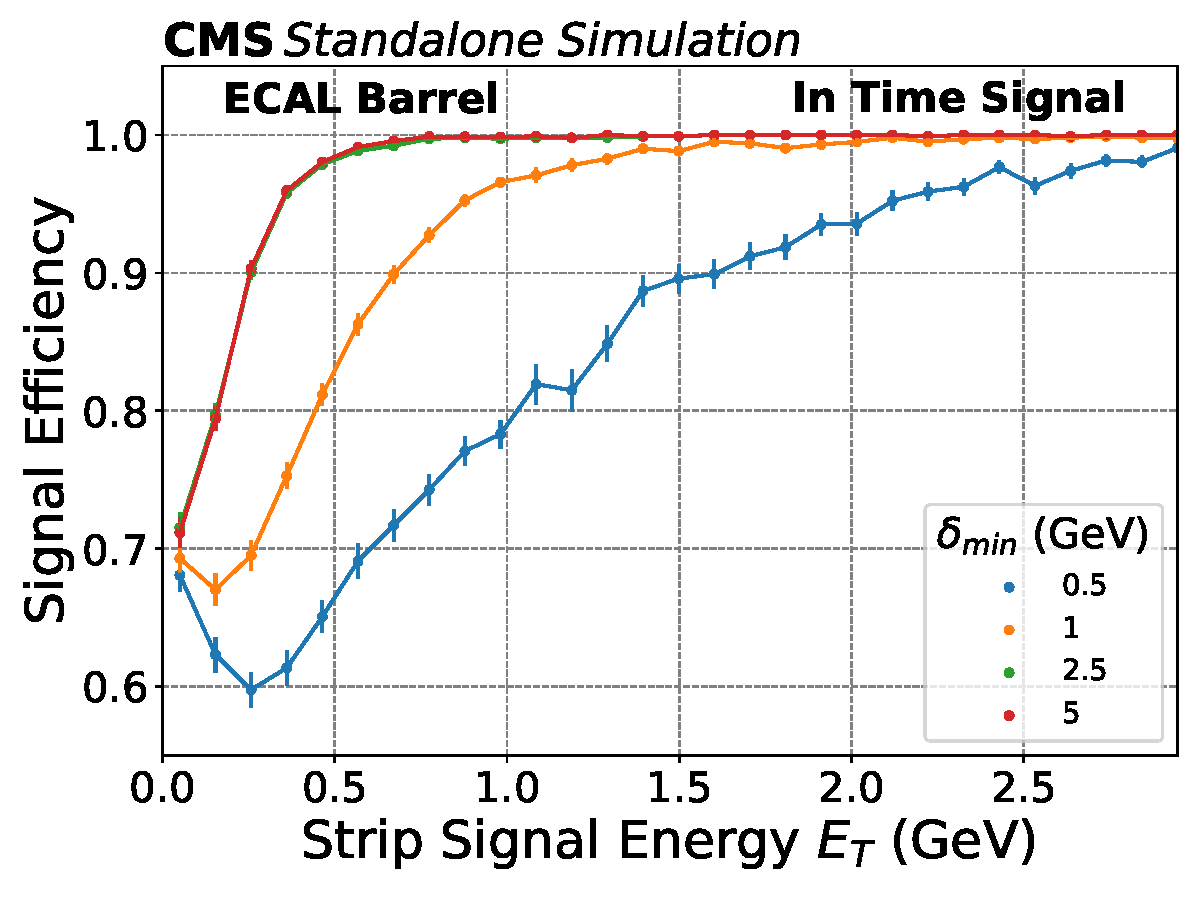
\includegraphics[width=0.8\textwidth]{Images/ECAL/DW/SigEff_vs_SigET.pdf}
    \caption{Signal efficiency vs. signal energy using a standalone simulation and simulation of ECAL double weights algorithm.}
    \label{fig:SimSignaltaggedvsE}
\end{figure}

It is observed that increasing the $\delta_{min}$ parameter value results in higher signal efficiency, as expected for the same reason that a greater spike rejection is observed for greater $\delta_{min}$ values: Only signal and spike waveforms which exhibit larger differences in EVEN and ODD amplitudes are used for weight optimization, leading to weights which are more optimized for very different waveforms and therefore less likely to touch signal waveforms. In order to identify a reasonable trade-off between signal efficiency and spike rejection, the resulting efficiencies are rejections for different $\delta_{min}$ working points is shown in Figure \ref{fig:SpikeRejSigEffTable}, where only signals with $E_{T} \leq 3$ GeV are considered as simulated signals with $E_{T} > $ 3 GeV have an efficiency near 100\%. Additionally, only spikes with a timing greater than 10 ns are considered, as these working points are not effective at tagging in-time spikes.

\begin{figure}
    \centering
        \begin{tabular}{|c|c|c|} \hline 
          $\delta_{min}$ (GeV) & Signal efficiency (\%) & Spike rejection (\%) \\ \hline 
         0.5 & 78.2 & 77.6 \\ \hline  
         2.5 & 95.6 & 62.5 \\ \hline 
         5.0 & 95.7 & 19.2 \\ \hline    
        \end{tabular}
    \caption{Signal efficiency and spike rejection for different $\delta_{min}$ working points.}
    \label{fig:SpikeRejSigEffTable}
\end{figure}

It is shown that moving from the $\delta_{min} = $ 2.5 GeV to 5.0 GeV working point returns a minimal gain in signal efficiency (0.1\%), while a large fraction of spike
rejection is lost (43.3\%). This indicates that the $\delta_{min} = 2.5$ GeV working point provides a good compromise between signal efficiency at low $E_{T}$ and overall spike rejection.

\subsection{Re-emulation of 2018 data} \label{sec:reEmuOf2018Data}

One of the ways to test new features during a long shutdown period when no new data is being taken is be re-emulating previously recorded data. As double weights were an undiscovered feature, they were not present in the CMS ECAL emulator. After verifying the existence of this feature in hardware through tests at CERN building 904 and at the CMS ECAL itself, the now confirmed second amplitude filter was added as a possible configuration in the CMS emulator \cite{CMSSW_DW}.

After including this implementation in the centrally used CMS software, 2018 CMS data was re-emulated using ECAL double weights in order to see how this would have affected data-taking. Double weights were run in "Killing mode", meaning that if an ECAL strip has a higher ODD amplitude than EVEN amplitude, its energy is set to zero. The idea behind this is to zero spikes which are often out-of-time, while trying to minimize the zeroing of signals which are in-time. 

In order to categorize ECAL TPs in data as signal-like or spike-like, an offline ``Severity" assignment is used. Each EB TT (Trigger tower) is composed of 25 ECAL crystals. An offline energy computation is performed for each crystal in highly energetic regions of events with an L1A, called a reconstructed hit or ``rec hit". In addition, a timing value is computed for each reconstructed hit, and a ``severity" level is assigned. A severity level of 0 corresponds to a reconstructed hit which does not appear problematic in the data. A severity level of 3 means a reconstructed hit is identified as out-of-time based on its reconstructed timing value, and a severity level of 4 means a reconstructed hit satisfies at least one of the following: Identified as out-of-time based on its reconstructed time value, fails a topological cut, known as a ``swiss-cross" cut. Because spikes come from isolated APD hits, rather than from a spread-out EM shower with energy spread over a group of ECAL crystals, spikes usually have their energy fully deposited in one crystal and are identified using a swiss cross variable, shown in Figure \ref{fig:SwissCross}. Thus, severity zero (four) reconstructed hits typically correspond to signal-like (spike-like) hits shown in its respective region of reconstructed time vs. swiss-cross score in Figure \ref{fig:TimeVsSwissCross} \cite{CMS-DP-2012-008, CMS-DP-2012-008_Plots}. 

\begin{figure}[H]%
    \setcounter{subfigure}{0}
    \centering
    \subfloat[Swiss cross definition, illustrated by the energy hits in a 3x3 ECAL crystal portion. E1 = energy of the central crystal, E4 = sum of the energies of the central crystal's four surrounding neighbors.  \label{fig:SwissCross}]{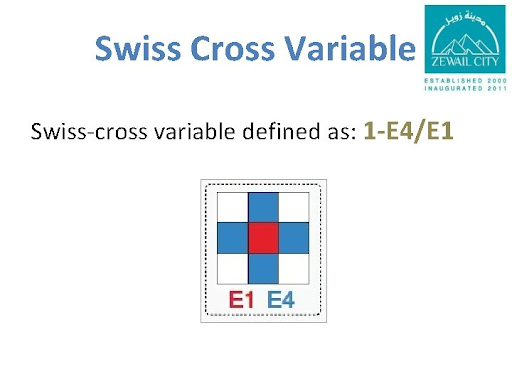
\includegraphics[width=.475\textwidth]{Images/ECAL/DW/SwissCross.png}}%
    \hfill
    \subfloat[Reconstructed time vs. swiss cross score \label{fig:TimeVsSwissCross}]{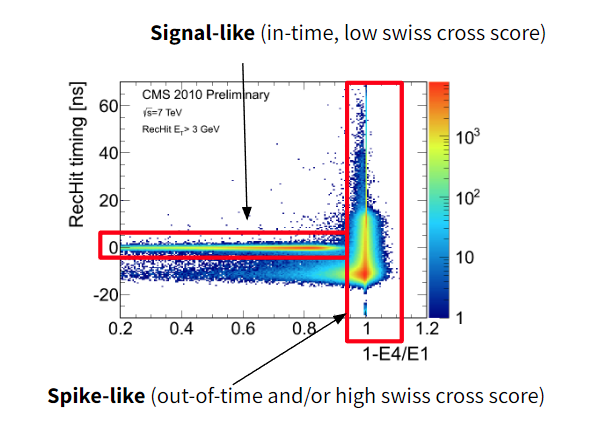
\includegraphics[width=.475\textwidth]{Images/ECAL/DW/timeVsSwissCross.png}}%
    \caption{Swiss cross definition, and reconstructed hit timing vs. swiss cross score from a 2010 CMS data sample.}%
\end{figure}

In order to assign a severity level and reconstructed time to an EB TP, the severity level and reconstructed time of the highest energy reconstructed hit in a given TP is assigned to that TP, as shown in Figure \ref{fig:RecHitTPMatching}. In this example TP with reconstructed crystal energies in arbitrary units, the highest energy reconstructed hit is in Strip 3, crystal 0 as its value is 201, and thus this TP is assigned the timing and severity of this crystal. 

\begin{figure}[H]
    \centering
    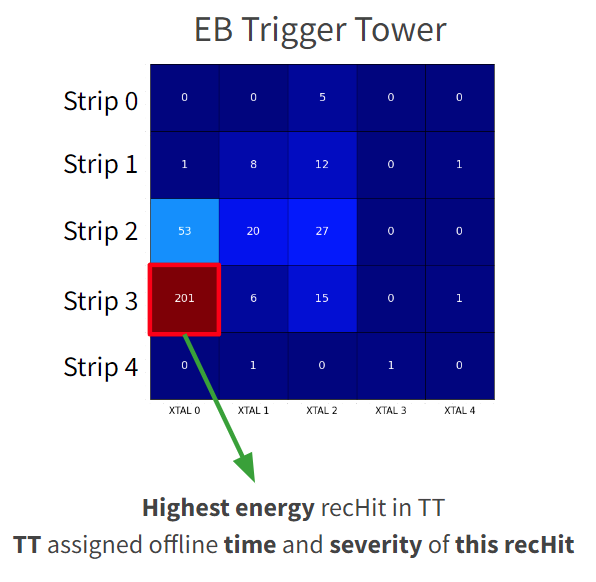
\includegraphics[width=0.8\textwidth]{Images/ECAL/DW/TPRecHitMatching.png}
    \caption{Reconstructed hit matching to TP. Crystal energy units are arbitrary.}
    \label{fig:RecHitTPMatching}
\end{figure}

In the re-emulation of 2018 CMS data, the resulting 1 - emu/real distributions, where emulated energy includes double weights in killing mode, and real energy corresponds to the energy of the TP from data with no double weights applied, are shown in Figure \ref{fig:2018Reemulation_KillingMode} for signals (TPs assigned to severity 0 reconstructed hits) which are in time (matched reconstructed crystal hit time $|t| < 3$ns), and spikes (TPs assigned to severity 4 reconstructed hits) which are out-of-time (matched reconstructed crystal hit time $t > 10$ns). 

\begin{figure}[H]%
    \setcounter{subfigure}{0}
    \centering
    \subfloat[2018 CMS data re-emulation, in time severity zero energies in killing mode \label{fig:DW_2018Reemulation_InTimeSevZeroKillingMode}]{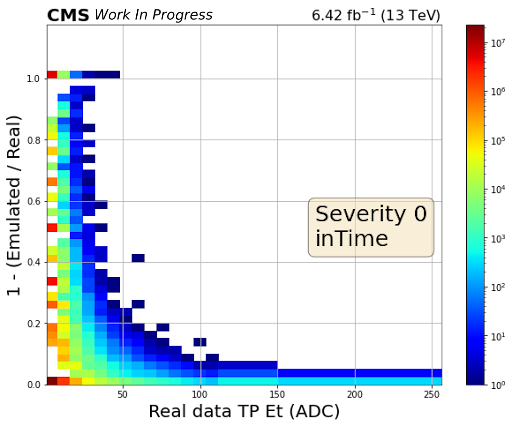
\includegraphics[width=.475\textwidth]{Images/ECAL/DW/DW_2018_Reemulation_InTimeSevZeroEnergies.png}}%
    \hfill
    \subfloat[2018 CMS data re-emulation, very late severity four energies in killing mode \label{fig:DW_2018Reemulation_VeryLateSevFourKillingMode}]{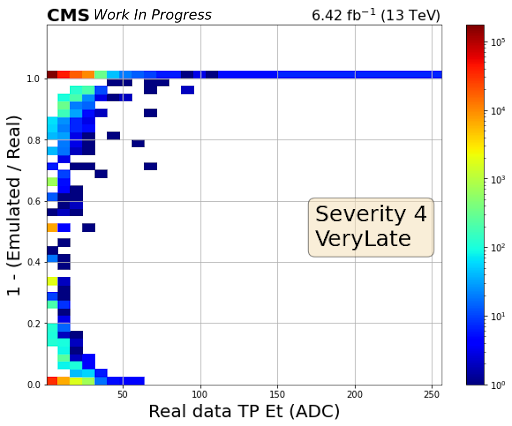
\includegraphics[width=.475\textwidth]{Images/ECAL/DW/DW_2018_Reemulation_VeryLateSevFourEnergy.png}}%
    \caption{2018 Data reemulation with double weights in killing mode. \label{fig:2018Reemulation_KillingMode}}%
\end{figure}

This shows that relatively high energy spikes, greater than about 50 ADC (25 GeV), are being mostly zeroed, shown by the fact that the 1 - emulated / real is close to one, meaning the emulated (TP energy with double weights in killing mode) energy is nearly zeroed. There is also a non-negligible amount of zeroing being applied to in-time signals, as the per y-slice distributions show some entries greater than 0. 

To check the timings of TPs which have some energy subtracted by double weights in the full timing range, not just restricted to in time and very later, we can observe the data TP vs. its offline assigned time for all TPs shown in Figures \ref{fig:All_Sev_zero} and \ref{fig:All_Sev_four}, and for TPs in which at least 90\% of energy is removed by double weights in killing mode in figures \ref{fig:MostlyZeroed_Sev_zero} and \ref{fig:MostlyZeroed_Sev_four}. For both severity categories, a line is drawn at 32 ADC, equivalent to 16 GeV for ECAL TPs, as this is the spike killing threshold as defined in Section \ref{sec:spikes}. 

\begin{figure}[H]%
    \setcounter{subfigure}{0}
    \centering
    \subfloat[All severity zero TPs \label{fig:All_Sev_zero}]{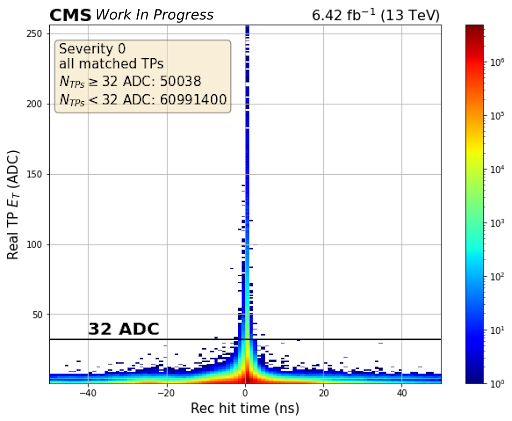
\includegraphics[width=.475\textwidth]{Images/ECAL/DW/DW_2018_Reemulation_AllSevZeroTPs.png}}%
    \hfill
    \subfloat[Severity zero TPs mostly zeroed \label{fig:MostlyZeroed_Sev_zero}]{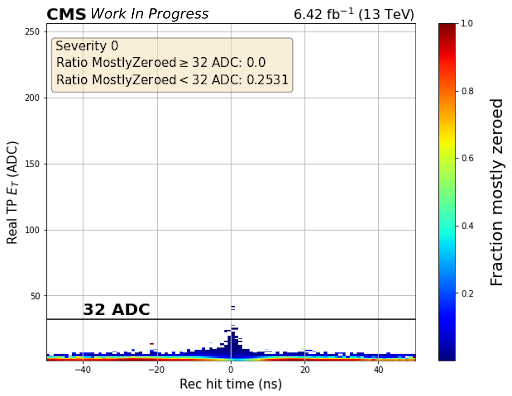
\includegraphics[width=.475\textwidth]{Images/ECAL/DW/DW_2018_Reemulation_SevZeroTPsMostlyZeroed.png}}%
    \caption{2018 Data reemulation - severity 0 TPs \label{fig:A}}%
\end{figure}

\begin{figure}[H]%
    \setcounter{subfigure}{0}
    \centering
    \subfloat[All severity four TPs \label{fig:All_Sev_four}]{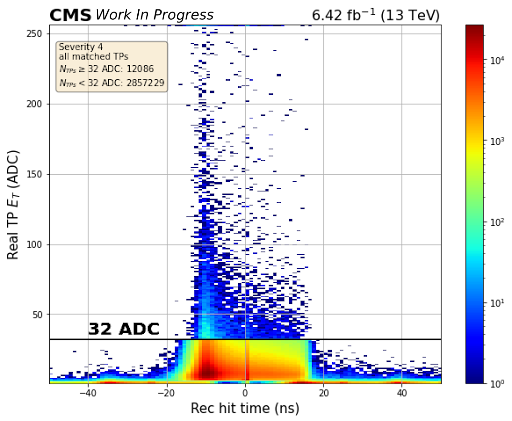
\includegraphics[width=.475\textwidth]{Images/ECAL/DW/DW_2018_Reemulation_AllSevFourTPs.png}}%
    \hfill
    \subfloat[Severity four TPs mostly zeroed \label{fig:MostlyZeroed_Sev_four}]{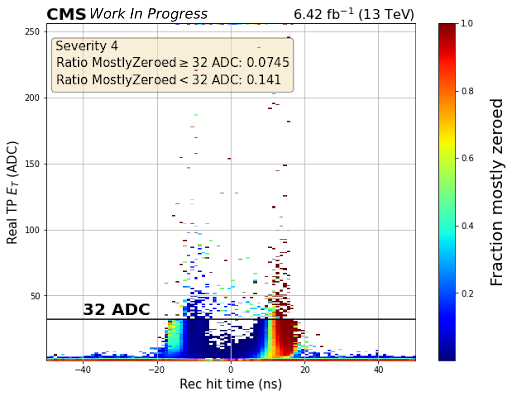
\includegraphics[width=.475\textwidth]{Images/ECAL/DW/DW_2018_Reemulation_SevFourTPsMostlyZeroed.png}}%
    \caption{2018 Data reemulation - severity 4 TPs \label{fig:A}}%
\end{figure}

In the distributions containing all TPs, most signals are in-time as expected. It is also observed that a large portion of spikes are out of time, as expected. It is observed that many spikes have a negative timing around -12.5ns, which is due to a bias in the ECAL offline energy reconstruction, which is optimized for signal waveforms which are slightly different from spike waveforms. Spike waveforms with a negative reconstructed time are generally expected to really be in time. Additionally, the effect of the spike killer is visible for severity four TPs, as there is a sharp drop-off in the number of TP entries above the spike killer threshold of 32 ADC (16 GeV). 

The distributions of TPs which have at least 90\% of their energy subtracted by double weights in killing mode show that most signal-like TPs which are mostly zeroed are very low energy and out of time, which are likely coming from noise, and it can be seen that there is a non-zero chance of some in-time signal energy subtraction. For spike TPs, it is seen that the majority of TPs which have their energy mostly subtracted are positively out of time, as expected with double weights based on the standalone simulation shown in Figure \ref{fig:DW_StandaloneSimulation_SpikeTimingPDFTagging}. The spike contamination of ECAL TPs, with and without double weights activated in killing mode, is shown in Figure \ref{fig:DW_2018Reemulation_SpikeContamination}. 

\begin{figure}[H]
    \centering
    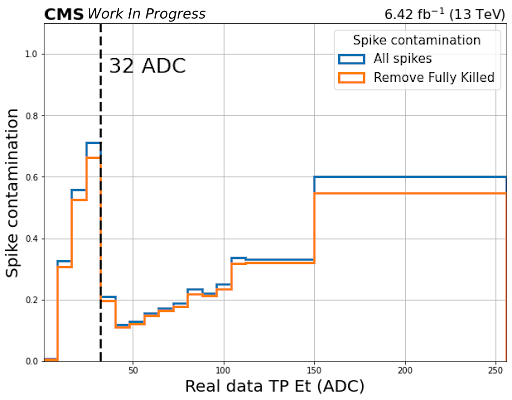
\includegraphics[width=0.8\textwidth]{Images/ECAL/DW/SpikeContamination_DoubleWeights.png}
    \caption{2018 CMS data re-emulation, expected improvement in spike contamination, including below the spike killer threshold.}
    \label{fig:DW_2018Reemulation_SpikeContamination}
\end{figure}

This shows that with ECAL double weights, there is some potential to lower the spike contamination rate, including in the high energy regime. This is also true for spikes with energy less than 32 ADC (16 GeV), the existing Level-1 spike killer threshold. 

While we see potential for a decrease in spike contamination, this re-emulation of 2018 CMS data also showed we may expect to have the unwanted removal of some signal energy at low TP energies with this double weights working point. In order to further study this, another re-emulation was performed with a full-readout ECAL run. The reason a full-readout run was included in this study is because in full-readout, information from all ECAL crystals is saved. In non full-readout runs, there is a selective readout procedure in which low interest regions are not readout. It is desirable to re-emulate full readout runs when comparing low energy TP energies between data and re-emulation, to ensure that all ECAL information is available for emulation in order to have a proper comparison to data. This re-emulation was performed with two double weights working points: $\delta_{min}$ = 0.5 and 2.5 GeV, running with double weights in killing mode. The resulting average energy fractions subtracted from in time signals and out-of-time spikes when re-emulating with these two working points are shown in Figure \ref{fig:2018Reemulation_FR_KillingMode_deltamincompare}. 

\begin{figure}[H]%
    \setcounter{subfigure}{0}
    \centering
    \subfloat[In time severity zero TPs \label{fig:2018Reemulation_FR_KillingMode_deltamincompare_InTimeSignals}]{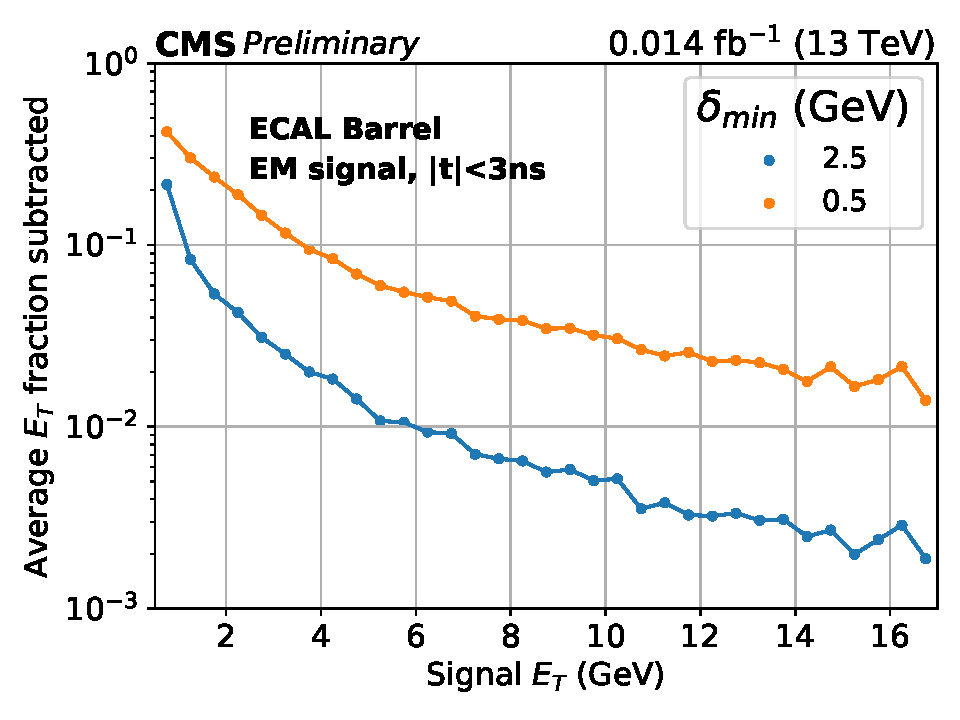
\includegraphics[width=.475\textwidth]{Images/ECAL/DW/Sev_zero_inTime_Average_oneMinusEmuOverRealvstwrADCCourseBinningZoomed_log.pdf}}%
    \hfill
    \subfloat[Very late severity four TPs \label{fig:2018Reemulation_FR_KillingMode_deltamincompare_VeryLateSpikes}]{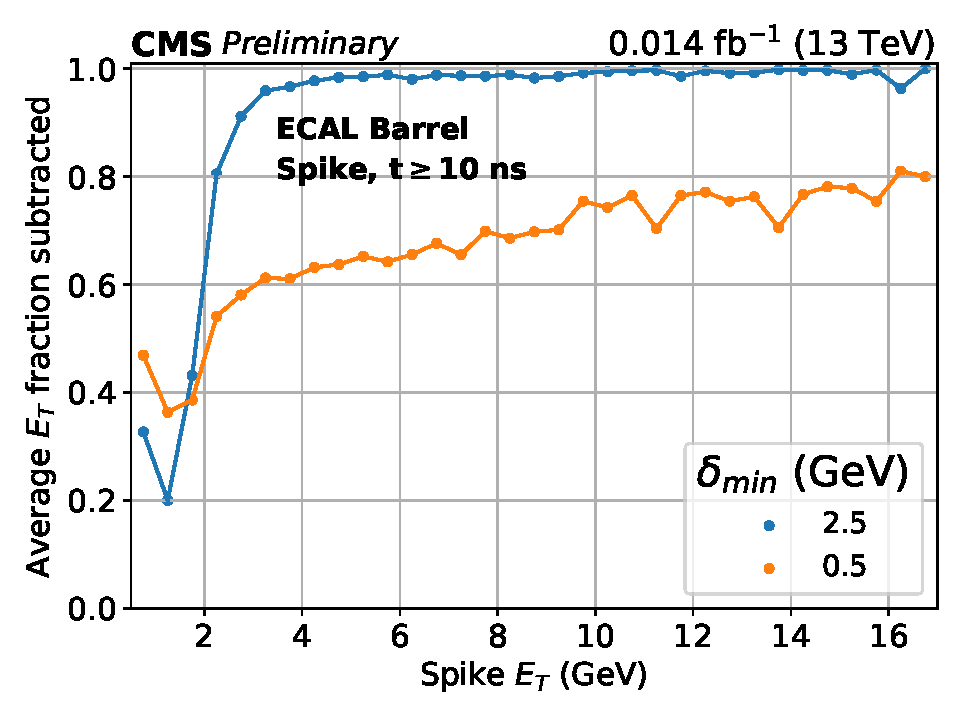
\includegraphics[width=.475\textwidth]{Images/ECAL/DW/Sev_four_VeryLate_Average_oneMinusEmuOverRealvstwrADCCourseBinningZoomed_linear.pdf}}%
    \caption{2018 Data reemulation, Full Readout run, with DW in killing mode. \label{fig:2018Reemulation_FR_KillingMode_deltamincompare}}%
\end{figure}

Firstly, this re-emulation with the $\delta_{min}$ = 0.5 GeV point shows similar trends observed in the previous study: Namely that low energy signals have a non-zero probability of having energy subtracted which decreases as the TP energy increases, and that out of time spikes have a large percentage of energy subtracted, which increases as spike energy increases. Secondly, both trends exhibit more desirable behavior with the $\delta_{min}$ = 2.5 GeV working point: The amount of signal energy subtraction is decreased, and the amount of spike energy subtraction is increased. These same trends were observed in the standalone simulation results in Figure \ref{fig:DW_StandaloneSimulation_SpikeTimingPDFTagging} for simulated spikes and Figure \ref{fig:SimSignaltaggedvsE} for simulated signals.

\subsection{Commissioning for LHC Run 3} \label{sec:ECALTrigger_Run3}

During the commissioning of CMS and LHC for Run 3, the accelerator complex provided beam splashes to the experiments, in which an LHC collimator upstream from CMS is closed, resulting in a proton bunch interaction and production of a shower of particles, chiefly muons, which traverse the entire CMS detector. An event display from a 2021 LHC beam splash is shown in Figure \ref{fig:2021PilotBeam_BeamSplash}, where red represents ECAL activity and blue represents HCAL activity. 

\begin{figure}[H]
    \centering
    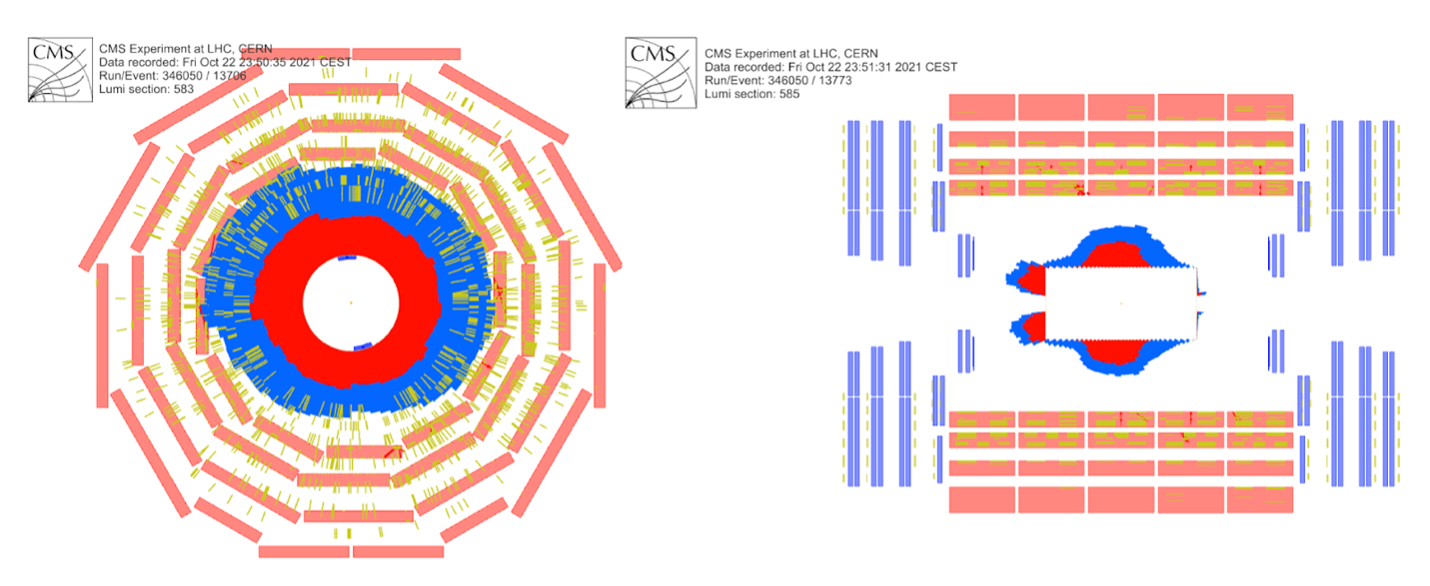
\includegraphics[width=\textwidth]{Images/ECAL/DW/BeamSplash.png}
    \caption{2021 LHC pilot beam: Beam splash}
    \label{fig:2021PilotBeam_BeamSplash}
\end{figure}

During beam splashes, a broad range of ECAL reconstructed hit timings are returned. This is because a shower of particles arrives at the detector from one direction, where CMS is configured to trigger the event from ECAL activity in the central region around $\eta$ = 0. This defines in-time hits in the detector, akin to the time of a proton-proton bunch collision, and because the shower of particles continues to interact with the rest of ECAL as time passes, all of these hits will be recorded as positively out-of-time. Additionally, all of the hits from the shower of particles which strikes ECAL before the event is triggered will be negatively out-of-time with respect to $\eta$ = 0.  

As this means a large range of timings for offline ECAL crystal reconstructed hits is expected which can be matched to ECAL TPs in the same fashion performed in \ref{sec:reEmuOf2018Data}, the ECAL operations team used the opportunity to run with double weights in tagging mode, in which no energy is subtracted but a flag is set if a TP is marked as out-of-time by the double weights mechanism. The resulting ECAL TP timings, and the TPs which were tagged are shown in Figure \ref{fig:2021_BeamSplash_DWTagging}. 

\begin{figure}[H]%
    \setcounter{subfigure}{0}
    \centering
    \subfloat[TP timing distribution]{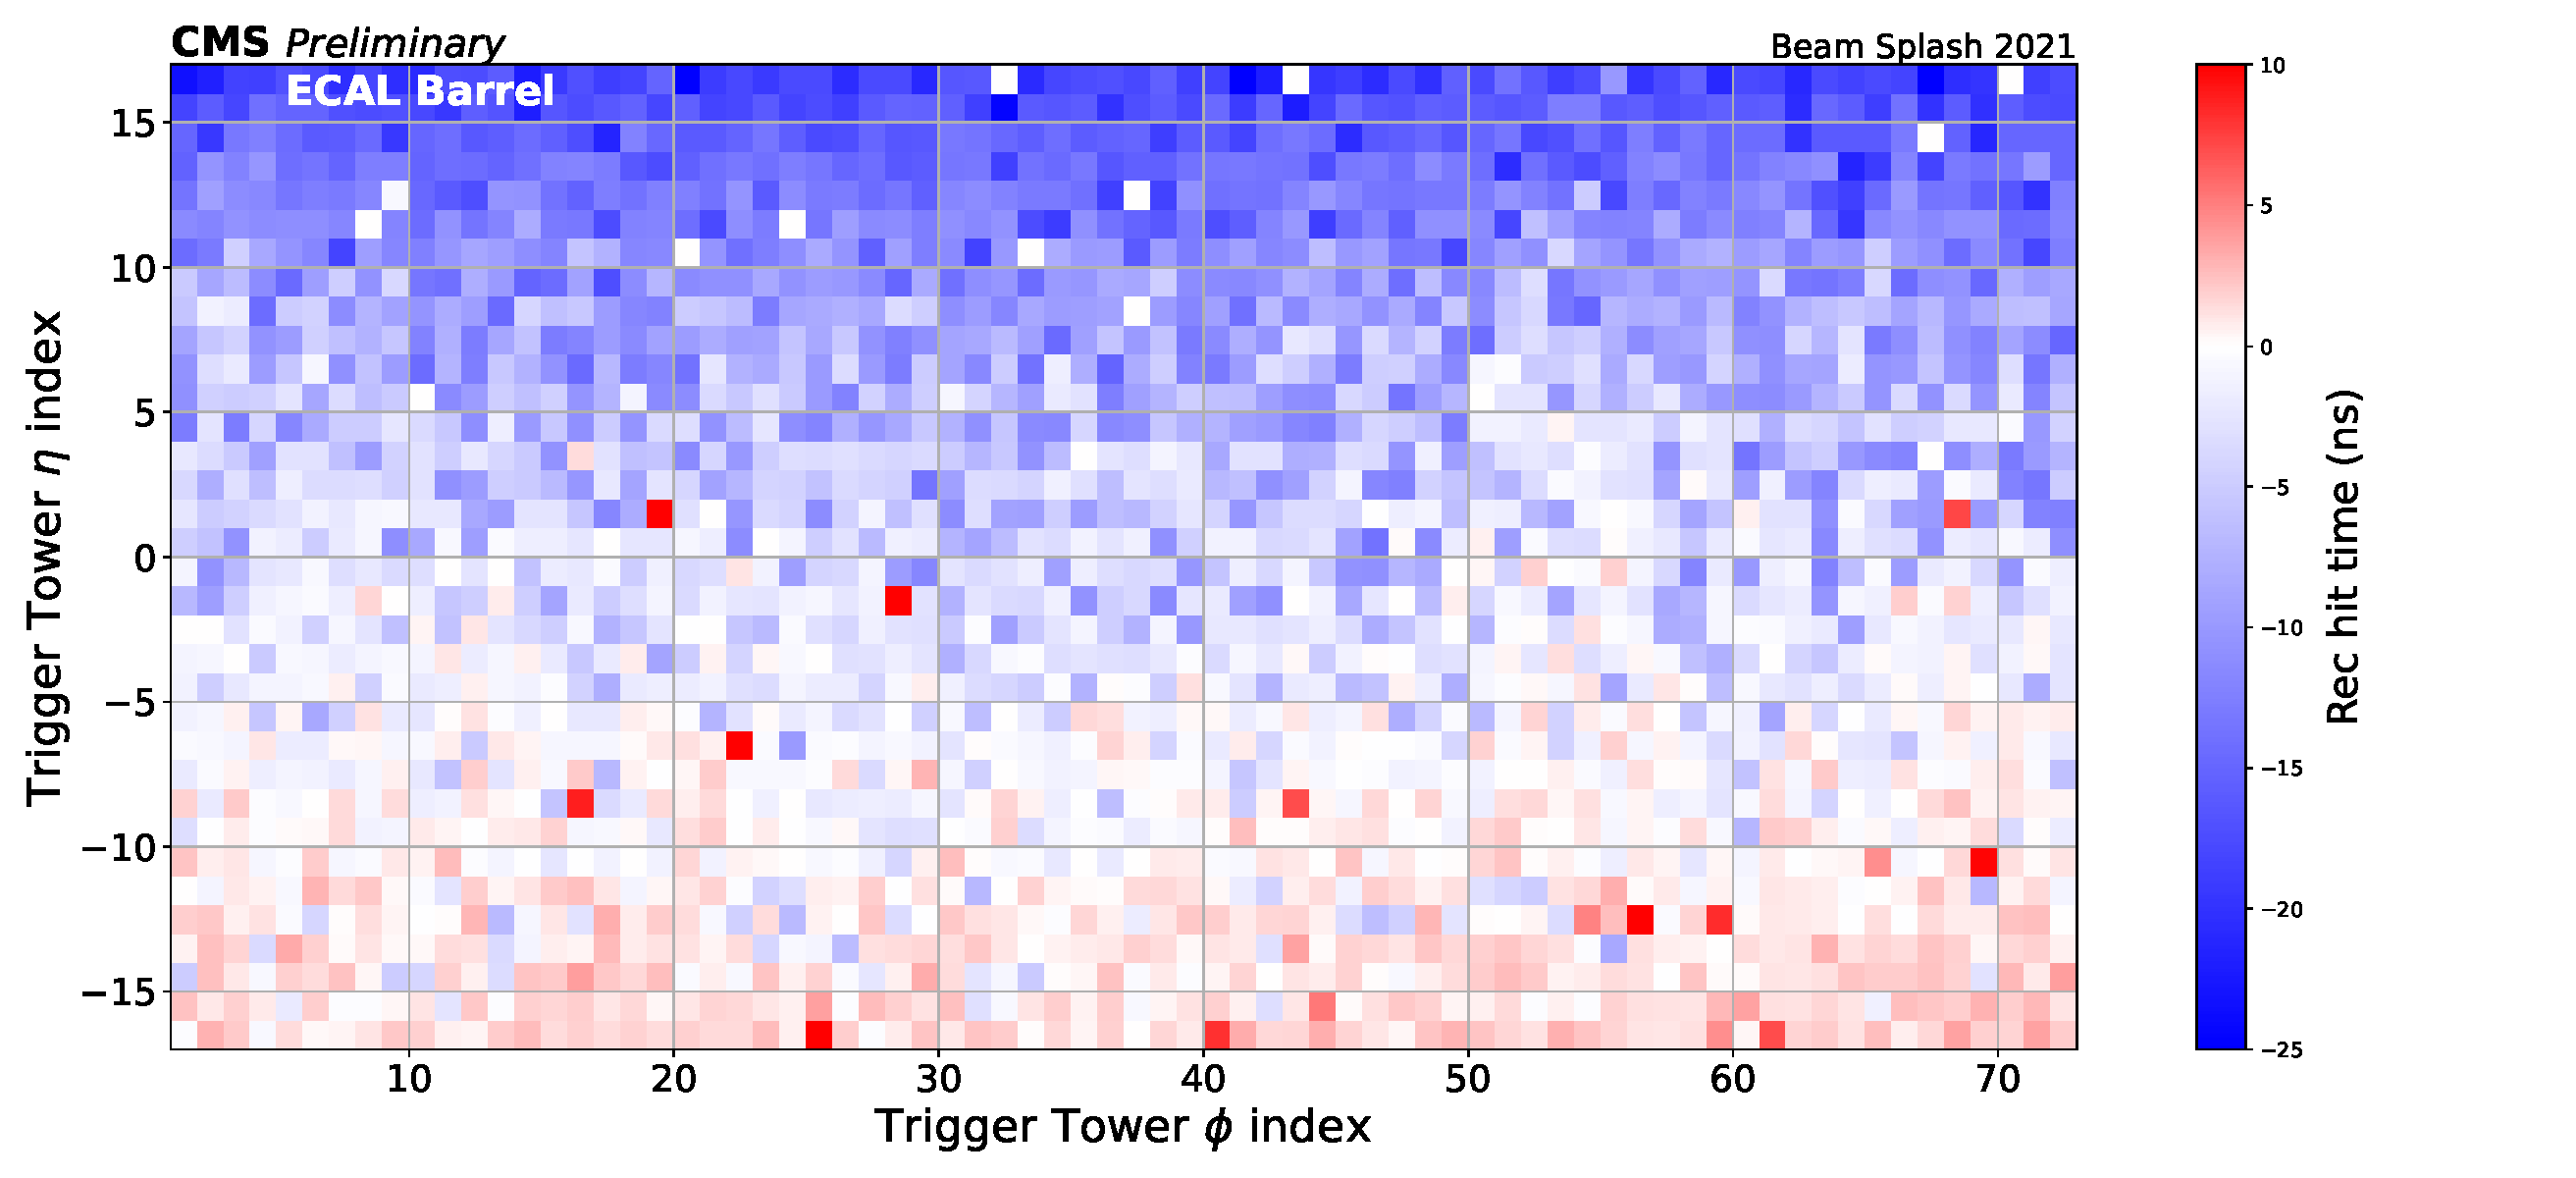
\includegraphics[width=.475\textwidth]{Images/ECAL/DW/BeamSplash2021_time.pdf}}%
    %\hfill
    \subfloat[TPs tagged as out of time]{\includegraphics[width=.475\textwidth]{Images/ECAL/DW/BeamSplash2021_FineGrainBit.pdf}}%
    \caption{TP timing distribution, and TPs which are tagged as out-of-time by the double weights mechanism, from a 2021 CMS beam splash. \label{fig:2021_BeamSplash_DWTagging}}%
\end{figure}  

It is observed that the TP timings, obtained by assigning the timing of the highest energy reconstructed hit in the TT, range from about -25ns to 10ns. The TPs which are tagged by the double weights mechanism as out-of-time have timings in the largely negative region of about -10 ns to -15 ns, with no tagging of in-time signals. This marked the first instance of out-of-time tagging at the ECAL TP level, and proved the functionality of the double weights mechanism for tagging out-of-time signals in data.

In addition, during the 2021 and 2022 LHC commissioning periods, CMS received low intensity 900 GeV center-of-mass energy collisions. During a 2 hour period, ECAL took data from these collisions in full readout mode running with double weights in tagging mode, in a 2021 run with the $\delta_{min}$ = 0.5 GeV working point, and in a 2022 run with the $\delta_{min}$ = 2.5 GeV working point. For the 2021 run, the data TP energies vs. offline matched times, and the fraction of TPs tagged over the total are shown in Figure \ref{fig:2021_Pilotbeam_TPsallAndTagged_sev0} for severity zero matched signal-like TPs, and Figure \ref{fig:2021_Pilotbeam_TPsallAndTagged_sev4} for severity 4 matched spike-like TPs. 

\begin{figure}[H]%
    \setcounter{subfigure}{0}
    \centering
    \subfloat[All severity 0 signal TPs: Data energy vs. time]{\includegraphics[width=.475\textwidth]{Images/ECAL/DW/2021PilotBeam_Energyvstime_sev0.png}}%
    \hfill
    \subfloat[Signal TPs tagged by double weights with $\delta_{min}$ = 0.5 GeV working point]{\includegraphics[width=.475\textwidth]{Images/ECAL/DW/2021PilotBeam_Energyvstime_sev0_tagged.png}}%
    \caption{2021 LHC pilot beam severity 0 signal TPs, all and tagged \label{fig:2021_Pilotbeam_TPsallAndTagged_sev0}}%
\end{figure}  

\begin{figure}[H]%
    \setcounter{subfigure}{0}
    \centering
    \subfloat[All severity 4 spike TPs: Data energy vs. time]{\includegraphics[width=.475\textwidth]{Images/ECAL/DW/2021PilotBeam_Energyvstime_sev4.png}}%
    \hfill
    \subfloat[Spike TPs tagged by double weights with $\delta_{min}$ = 0.5 GeV working point]{\includegraphics[width=.475\textwidth]{Images/ECAL/DW/2021PilotBeam_Energyvstime_sev4_tagged.png}}%
    \caption{2021 LHC pilot beam severity 4 spike TPs, all and tagged \label{fig:2021_Pilotbeam_TPsallAndTagged_sev4}}%
\end{figure}  

From these distributions, similar behavior is observed compared to that from the 2018 non full-readout and full-readout data re-emulation: Double weights are able to tag TPs which are positively out-of-time, as well as some spikes which are negatively out of time. For signals, there is a non-negligible amount of tagging seen for in-time signals. As the $\delta_{min}$ = 2.5 GeV working point was seen in 2018 re-emulation to have decreased signal tagging and increased spike tagging, the 2022 run with this working point is compared to the 2021 run as shown in Figure \ref{fig:2021_2022_900GeVCollisions_inTimeSignalTagging} for in-time severity 0 matched TPs, and Figure \ref{fig:2021_2022_900GeVCollisions_VeryLateSpikeTagging} for very late severity 4 matched TPs.

\begin{figure}[H]%
    \setcounter{subfigure}{0}
    \centering
    \subfloat[Linear y-scale]{\includegraphics[width=.475\textwidth]{Images/ECAL/DW/Sev_zero_inTime_Average_EnergyVsTimeOccupancy_linear.png}}%
    \hfill
    \subfloat[Logarithmic y-scale]{\includegraphics[width=.475\textwidth]{Images/ECAL/DW/Sev_zero_inTime_Average_EnergyVsTimeOccupancy_log.png}}%
    \caption{Tagging probability of in-time signal TPs as a function of TP transverse energy, with two double weights working points, shown in linear and logarithmic y-scale. \label{fig:2021_2022_900GeVCollisions_inTimeSignalTagging}}%
\end{figure}  

\begin{figure}[H]
    \centering
    \includegraphics[width=0.9\textwidth]{Images/ECAL/DW/Sev_four_VeryLate_Average_EnergyVsTimeOccupancy_linear.png}
    \caption{Tagging probability of in-time signal TPs as a function of TP transverse energy, with two double weights working points.}
    \label{fig:2021_2022_900GeVCollisions_VeryLateSpikeTagging}
\end{figure}

This comparison returns similar behavior compared to the 2018 full readout re-emualtion shown in Figure \ref{fig:2018Reemulation_FR_KillingMode_deltamincompare}, as the $\delta_{min}$ = 2.5 GeV working point has less in time signal tagging which decreases as energy increases, and more late spike tagging which increases as energy increases.

In order to ensure that the emulator is properly simulating the ECAL double weights tagging mechanism as observed in data, a comparison of the tagging by data and the emulator was investigated for these two low energy runs, shown in Figure \ref{fig:SevZeroDataEmulatorTagging} for in-time severity 0 matched TPs, and Figure \ref{fig:SevFourDataEmulatorTagging} for very late severity 4 matched TPs.

\begin{figure}[H]%
    \setcounter{subfigure}{0}
    \centering
    \subfloat[2021 collisions, $\delta_{min}$ = 0.5 GeV working point ]{\includegraphics[width=.475\textwidth]{Images/ECAL/DW/2021Collisions_Sev_zero_inTime_DataOverEmulatorTaggingProbability_linear.png}}%
    \hfill
    \subfloat[2022 collisions, $\delta_{min}$ = 2.5 GeV working point]{\includegraphics[width=.475\textwidth]{Images/ECAL/DW/2022Collisions_Sev_zero_inTime_DataOverEmulatorTaggingProbability_linear.png}}%
    \caption{Tagging probability in data and as computed by the emulator for Severity 0 matched TPs with offline matched reconstructed times $|t| < $ 3 ns. \label{fig:SevZeroDataEmulatorTagging}}%
\end{figure}  

\begin{figure}[H]%
    \setcounter{subfigure}{0}
    \centering
    \subfloat[2021 collisions, $\delta_{min}$ = 0.5 GeV working point]{\includegraphics[width=.475\textwidth]{Images/ECAL/DW/2021Collisions_Sev_four_VeryLate_DataOverEmulatorTaggingProbability_linear.png}}%
    \hfill
    \subfloat[2022 collisions, $\delta_{min}$ = 2.5 GeV working point]{\includegraphics[width=.475\textwidth]{Images/ECAL/DW/2022Collisions_Sev_four_VeryLate_DataOverEmulatorTaggingProbability_linear.png}}%
    \caption{Tagging probability in data and as computed by the emulator for Severity 4 matched TPs with offline matched reconstructed times $>$ 10 ns. \label{fig:SevFourDataEmulatorTagging}}%
\end{figure}  

For the in time severity zero matched TP cases shown in Figure \ref{fig:SevZeroDataEmulatorTagging}, the tagging probabilities as evaluated by the data and emulator are in agreement within 0.6\%. This indicates that for the most part, the emulator can be trusted for accurately estimating the performance of the double weights mechanism on in-time severity zero matched TPs when re-emulating CMS data. 

For the late severity four matched TP cases shown in Figure \ref{fig:SevFourDataEmulatorTagging}, in the 2021 data sample there is one TP with disagreement in data and emulator energy in the 11 GeV bin. This individual TP requires further investigation to understand if this disagreement is due to the double weights mechanism or not. Apart from this TP, the double weights tagging probability as determined by data and the emulator are in agreement within 1.4\%, and fully in agreement for highly energetic TPs. In the 2022 data, there are a number of TPs which different data and emulated energies, which may or may not change the tagging probabilities computed in the data and emulator, which disagree by about 10\%. These differences require further investigation: They may be found to be due to the double weights in which the algorithm or weight values may need to be updated, or there may be an issue in the emulator which would need to be fixed.

Finally, during 2022 the LHC provided further beam splashes to CMS. The ECAL operations teams took this opportunity to run with double weights in ``killing $+$ tagging" mode, in which ECAL strips which have a greater ODD amplotide than EVEN amplitude have their energy zeroed (killing), and if there is a large amount of zeroing in a given ECAL TP, a flag is set (tagging). The functionality of this configuration was tested as it may be a potentially useful mode to use in the future, for instance to have the information of which regions of ECAL have their energy at least partially killed by double weights. An event from a 2022 beam splash running with ECAL double weights in killing $+$ tagging mode is shown in Figure \ref{fig:2022_BeamSplash_DWTagging}. 

\begin{figure}[H]%
    \setcounter{subfigure}{0}
    \centering
    \subfloat[TP energy distribution]{\includegraphics[width=.475\textwidth]{Images/ECAL/DW/BeamSplash2022_DW_TagNKill_Energy.png}}%
    %\hfill
    \subfloat[TPs tagged as out of time]{\includegraphics[width=.475\textwidth]{Images/ECAL/DW/BeamSplash2022_DW_TagNKill_Tagging.png}}%
    \caption{ECAL TP energies and TPs tagged as out-of-time by double weights in killing $+$ tagging mode during a 2022 CMS beam splash. \label{fig:2022_BeamSplash_DWTagging}}%
\end{figure} 

In this configuration, the majority of the ECAL barrel ran with its nominal Run 2 configuration, but killing $+$ tagging mode was set for two supermodules in the center of the detector. In one supermodule in which negatively out-of-time signals are expected, it is observed that there is some amount of killing of energy as the energy in that region is lower than the other supermodules with similar TP times, as the particle from the splash propagate from -$\eta$ to $+\eta$ and are expected to have roughly the same timing per $\eta$ index, and it can be seen that TPs in the same region are tagged. This is the first instance of ECAL running with double weights in killing $+$ tagging mode, and shows that this previously untested configuration appears to work as expected. 

While these initial re-emulation and data checks with double weights show potential gain at the ECAL TP level, as high energy spikes are tagged and removed while there is a minimal impact on low in-time signals and the emulator appears to provide an accurate representation of the double weights mechanism applied to in time signal-like TPs, the next necessary thing to check is the impact of double weights on CMS L1 quantities. This includes the effect on L1 rates, and L1 turn-on curves. A potential gain would be a decrease in the L1 rates due to the removal of spikes, which may allow for a lowering of the L1 seed energy thresholds. This would potentially allow for the collection of more Higgs pair production events in electromagnetic final states, including HH$\rightarrow$WW$\gamma\gamma$, which may improve the sensitivity of this and other Higgs pair production analyses to be performed at CMS using the LHC Run 3 dataset. 

% %https://indico.cern.ch/event/418639/contributions/1018397/attachments/868759/1216511/proceeding.pdf

% \section{Operations} \label{sec:ECAL_Operations}

In order to take take quality data at the CMS ECAL and test the re-optimized and new features of the ECAL trigger for LHC Run 3, a variety of operations teams is necessary. The CMS ECAL operations are subdivided into various operations groups, as there is a wide array of areas of technology and expertise required in order to successfully operate the ECAL for data-taking. Each group covers a different aspect of ECAL, all with the goal of minimizing the downtime of the experiment and ensuring quality data is taken. There are many sides to the operation of ECAL, for each of which the corresponding operations team is crucial, and all must remain vigilant for the successful operation and maintenance of ECAL. 

\subsection{Technical Coordination}

The purpose of the ECAL Technical Coordination (TC) is to ensure the safe operation of all hardware components of ECAL, both those stored in the Underground Experimental Cavern (UXC), and Underground Service Cavern (USC). In the event of a major hardware failure, or cooling related issue which may occur and possibly prevent ECAL from running in a safe state, the TC team leads the effort in repairing these components and is responsible for notifying the rest of the ECAL operations group that a particular partition of ECAL is unavailable. During periods of collisions, and especially during long shutdown or technical stop periods, CMS TC coordinates a vast number of physical interventions to repair, upgrade, and service the detector. This large coordination effort requires a deep understanding of the physical architecture and history of ECAL, as well as an understanding of how an intervention on one CMS subdetector may affect another CMS subdetector. The role of the ECAL TC team includes following the planned CMS TC activities, as this may have implications on partitions of ECAL. An example CMS underground plan of the day is shown in Figure \ref{fig:CMS_TC_Example}.

\begin{figure}[H]
    \centering
    \includegraphics[width=0.85\textwidth]{Images/ECAL_Operations/CMS_TC_Example.png}
    \caption{Example plan of the day in CMS UXC/USC from 27 May 2021.}
    \label{fig:CMS_TC_Example}
\end{figure}

As an example, during a long LHC shutdown period there may be a day when one of the CMS endcaps must be physically moved in order to allow for an intervention on the inner hardware of another sub-detector which is not accessible when the detector is closed. This has an implication of the ECAL endcaps, as they may need to be powered off during this time to ensure the safety of the electronics. In a case like this, ECAL TC would report this required action of powering off to the rest of the ECAL operations teams in order for all to be aware that one endcap will not be available for a certain period of time. This can then potentially delay planned tests on this endcap, and is therefore essential information for the entire ECAL operations group to be aware of. 

\subsection{Detector Control System}

% https://indico.cern.ch/event/1122238/contributions/4711434/attachments/2380818/4067982/TrainingSession%20ECAL%20DCS%20Operators.pdf

The ECAL Detector Control System (DCS) team maintains, develops, and operates the ECAL DCS in order to ensure the proper control and safety of the detector. An image of the ECAL DCS monitor is shown in Figure \ref{fig:ECAL_DCS_Monitor}, displaying the powering status of the full ECAL and ES as ON. 

\begin{figure}[H]
    \centering
    \includegraphics[width=0.85\textwidth]{Images/ECAL_Operations/ECAL_DCS.png}
    \caption{ECAL DCS monitor}
    \label{fig:ECAL_DCS_Monitor}
\end{figure}

In the example situation in which there is activity in UXC which requires the powering off of an ECAL Endcap, a request would be made to the ECAL DCS operator to use the DCS in order to power off the desired partition of ECAL. In the event in which issues during this powering off may occur, the operator follows a pre-defined set of protocols in order to safely identify and solve the encountered issue without harming the detector.  

\subsection{Run Coordination}

The purpose of ECAL Run Coordination (RC) is to coordinate the running operations of ECAL, including all times during which the detector is powered on. This primarily involves the planning of tests, coordination between ECAL and CMS, and training of on-call ECAL shifters in order to carry out operation plans. A diagram illustrating the paths of communication between ECAL and CMS during running can be seen in Figure \ref{fig:ECAL_CMS_RC_diagram}.

\begin{figure}[H]
    \centering
    \includegraphics[width=0.85\textwidth]{Images/ECAL_Operations/ECAL_RC_Diagram.png}
    \caption{ECAL / CMS running communication paths.}
    \label{fig:ECAL_CMS_RC_diagram}
\end{figure}

On a given day, the CMS run coordinators and Run Field Manager (RFM) make a plan of the day based on the plan of LHC and the requests of the individual subdetectors. It is the job of ECAL RC to make sure the requests made to CMS are consistent with the opinions and availability of the ECAL experts, and to then understand and share the implications of the CMS plan of the day on the ECAL subdetector. This may include planned tests for ECAL which use the CMS DAQ (Data AcQuisition) system, or the participation of ECAL in the tests of other CMS subsystems. It is essential for all participants in run coordination communications to execute fast and clear communication of information in order to minimize detector downtime, and optimize the use of commissioning and data-taking periods. 

\subsection{Data Acquisition} \label{sec:ECAL_DAQ}

% https://indico.cern.ch/event/1122210/contributions/4711234/attachments/2394725/4094305/ECAL_DAQ_Tutorial_for_DOCs_2021.pdf
% https://ecal-daq-doc.docs.cern.ch/
% https://gitlab.cern.ch/ecal-daq/ecal-daq-documentation/-/tree/master/docs/images

The ECAL DAQ (Data AcQuisition) team is responsible for ensuring effective data-taking by ECAL. A diagram of the ECAL DAQ path is shown in Figure \ref{fig:ECAL_DCC_Diagram}. 

\begin{figure}[H]
    \centering
    \includegraphics[width=0.85\textwidth]{Images/ECAL_Operations/ECAL_DCC_Diagram.png}
    \caption{ECAL DAQ path}
    \label{fig:ECAL_DCC_Diagram}
\end{figure}

Generally speaking, the data flow which takes place due to an energetic ECAL goes as follows: An energetic electromagnetically interacting particle produces scintillation light in the ECAL crystals (left-most side of Figure \ref{fig:ECAL_DCC_Diagram}), which reaches the crystals' photo-detectors (or an EB APD may be directly struck, leading to a spike which may fake an energetic ECAL signal). The signals from the photo-detectors are propagated through the VFE (very front end) cards, where in EB a set of five cards is connected to a single FE (front end card) for a 25 crystal TT, or a range of 1-25 crystals in EE. If an L1A is sent to the FE based on the CMS L1 trigger, the L1A will be received via the control token ring, triggering ECAL to readout its data first sending it to the DCC (data concentrator card), and then to the central CMS DAQ system to be processed at HLT. 

The ECAL DAQ team is additionally responsible for maintaining a slew of monitors used for monitoring various DAQ related quantities, to ensure that data acquisition is flowing as expected. An example is the ECAL payload monitor, used to monitor if very large amounts of data are being processed through each ECAL FED (Front end driver), corresponding to different parts of the detector (one supermodule in EB). The contents of this monitor during an ECAL full readout run, during a special run in which ECAL was running with double weights in tagging mode with the $\delta_{min}$ = 2.5 GeV working point as described in Section \ref{sec:ECALTrigger_Run3}, is shown in Figure \ref{fig:PayloadMonitor_ECAL} for ECAL, and \ref{fig:PayloadMonitor_ES} for the preshower.

\begin{figure}[H]
    \centering
    \includegraphics[width=\textwidth]{Images/ECAL_Operations/PayloadMonitor.png}
    \caption{ECAL payload monitor during a June 2022 full-readout run. On the y-axis, the size of a FED's payload fragment is plotted. On the x-axis, the ECAL FED number is plotted. Each FED number corresponds to an ECAL supermodule, and ranges from 601-654.}
    \label{fig:PayloadMonitor_ECAL}
\end{figure}

\begin{figure}[H]
    \centering
    \includegraphics[width=\textwidth]{Images/ECAL_Operations/PayloadMonitor_ES.png}
    \caption{ES payload monitor during a June 2022 full-readout run. On the y-axis, the size of a FED's payload fragment is plotted. On the x-axis, the ES FED number is plotted. Each FED number corresponds to a portion of ES.}
    \label{fig:PayloadMonitor_ES}
\end{figure}

Notably, the payloads in the ECAL barrel appear to be greater on average than the payloads in the ECAL endcaps. This may potentially be due to the fact that there are more readout channels in the EB (61,200 crystals compared to 14,648). 

\subsection{Trigger}

The primary role of the ECAL trigger team is to ensure the smooth operation and proper calibration of ECAL trigger primitive generation. Responsibilities include the identification and masking of noisy or problematic towers, the monitoring of ECAL's contribution to the CMS trigger rate, and the testing and commissioning of new features and protocols for future data-taking periods. A diagram of the ECAL trigger primitive generation path is shown in Figure \ref{fig:ECAL_TCC_Diagram}.

\begin{figure}[H]
    \centering
    \includegraphics[width=0.85\textwidth]{Images/ECAL_Operations/ECAL_TCC_Diagram.png}
    \caption{ECAL trigger primitive path}
    \label{fig:ECAL_TCC_Diagram}
\end{figure}

While data is first sent to the FE card as described in the previous Section \ref{sec:ECAL_DAQ}, it is stored on the FE electronics buffers while a trigger primitive is formed and sent to the TCC (Trigger concentrator card). The TCC passes the TPs to the calorimeter layers of L1, while the FE waits to receive, or not receive an L1A. 

\subsection{Electronics}

The ECAL electronics team is responsible for the maintenance of the ECAL on- and off- detector electronics. The main off-detector ECAL electronics modules are the TCC (Trigger Concentrator Card), CCS (Clock and Control system), and DCC (Data Concentrator Card). In the ECAL Barrel (EB), there is one TCC, CCS, and DCC per supermodule. By monitoring ECAL electronics, and performing physical maintenance such as the cleaning of electronics fibers or uploading of updated firmware when necessary, the ECAL electronics experts ensure the robustness and ability of the ECAL electronics to take quality data. 

% https://cmsdoc.cern.ch/~jlfaure/OD_Web_Folder/June-02/CCS-veryprelimspecs.pdf

\subsection{Laser and LED}

Due to radiation received by LHC delivered collisions, the transparency of ECAL crystals degrades over time due to radiation damage. A laser correction system is in place in order to measure and correct for losses in ECAL crystal transparency, as shown over the course of LHC Runs 1 and 2 in Figure \ref{fig:ECAL_Laser_History}. It can also be seen that during long shutdown periods without collisions, the ECAL crystals anneal and recover some transparency, as seen by the slight increases in transparency before and after a shutdown period.

\begin{figure}[H]
    \centering
    \includegraphics[width=\textwidth]{Images/ECAL_Operations/ECAL_Laser_History.png}
    \caption{ECAL crystal transparency history during LHC Runs 1 and 2.}
    \label{fig:ECAL_Laser_History}
\end{figure}

While similar shapes are observed for different $\eta$ regions of the detector, more radiation is received at higher $\eta$ regions, leading to lower transparency with respect to that from the start of LHC Run 1. In the highest pseudo-rapidity region in the last EE rings 2.7 $< \eta$, the crystals have an average transparency down to $\approx$ 4\% with respect to their original transparency. The high levels of radiation damage in the high $\eta$ regions are consistent with the higher amplitude fractional bias shown in Figure \ref{fig:ampBiasvseta}, and is one of the motivations for replacing the ECAL EE for the Phase-II CMS detector in favor of a new endcap detector called HGCAL (High granularity calorimeter).

An additional transparency measurement is taken by the LED for the ECAL endcaps. The ECAL laser team is responsible for ensuring the smooth operation of the ECAL laser and LED systems, which take crucial measurements to monitor the ECAL crystals and calibrate their outputs. 

\subsection{Data quality monitor} \label{sec:ECAL_DQM}

The purpose of the ECAL Data Quality Monitor (DQM) group is to maintain and develop the ECAL DQM plots used by both the central CMS DQM monitoring page, and the local version used privately by ECAL. An example set of DQM plots is shown in Figure \ref{fig:ECAL_DQM_Plots}. 

\begin{figure}[H]
    \centering
    \includegraphics[width=0.75\textwidth]{Images/ECAL_Operations/ECAL_DQM_Plots.png}
    \caption{Example ECAL DQM plots}
    \label{fig:ECAL_DQM_Plots}
\end{figure}

These plots are essential for monitoring the quality of data being taken by ECAL. If large sections of ECAL DQM plots show issues, typically colored red, it may hint at a problem which can be confirmed by going through additional DQM plots in order to better understand the underlying issue. This information would then be propagated to the appropriate ECAL experts in order to take the necessary action, such as fixing a certain piece of hardware or software. It is then checked if a problem has been solved by starting a new run, and confirming that the DQM plots no longer indicate an issue.  

\subsection{Prompt feedback group}

The role of the ECAL Prompt Feedback Group (PFG) is the provide prompt feedback regarding the quality of ECAL data. One of the main roles of the PFG group is to provide daily reports to the entire ECAL operations team, notifying everyone of the general status of ECAL based on a variety of monitoring plots, largely from the DQM previously described in Section \ref{sec:ECAL_DQM}. This daily report is crucial for catching any clear issues in ECAL data-taking, which may affect large portions of CMS data if left un-noticed. 

\subsection{Detector performance group}

The role of the ECAL Detector Performance Group (DPG) includes the maintenance, and improvement in quality of calibration applied to ECAL data. This also includes the tracking of physics performance of the ECAL detector, which can for instance be checked by analyzing the reconstruction of expected physics processes such as $\pi_{0}\rightarrow\gamma\gamma$, shown for runs from a 2022 commissioning period in black and a 2018 data taking period in blue in Figure \ref{fig:piZero_peak_13p6UnstableCollisions}.

\begin{figure}[H]
    \centering
    \includegraphics[width=0.85\textwidth]{Images/ECAL_Operations/pi0peak.png}
    \caption{Invariant mass of a diphoton pair from a $\pi_{0}$ candidate in EB during a 2022 commissioning run (black) and 2018 data-taking run (blue).}
    \label{fig:piZero_peak_13p6UnstableCollisions}
\end{figure}


\subsubsection{The Hadronic Calorimeter}\label{sec:HCAL}

% arxiv 1910.00079
% https://arxiv.org/pdf/1706.04965.pdf
% https://cms.cern/detector/measuring-energy/energy-hadrons-hcal

The CMS hadronic calorimeter is a sampling calorimeter composed of plastic scintillator and brass, whose purpose is to measure the energies of hadrons. This measurement is crucial for detecting clusters of hadronic energy, which can be matched with regions of high track activity in the identification of jets. 

A diagram of the HCAL layout during the start of Run 2 is shown in Figure \ref{fig:HCAL_Layout}. 

\begin{figure}[H]
    \centering
    \includegraphics[width=0.7\textwidth]{Images/CMS/HCAL/Figure_001.pdf}
    \caption{CMS HCAL layout in 2016}
    \label{fig:HCAL_Layout}
\end{figure}

The HCAL is composed of a hadron barrel (HB), hadron endcap (HE), hadron outer (HO), and hadron forward (HF) sections. HB (HE) has a pseudorapidity coverage of $|\eta| < 1.3$ ($1.3 < |\eta| < 3.0$). HO provides additional measurements in the barrel range, and the HCAL is complimented by HF which extends the angular coverage up to about $|\eta| = 5$. This is very useful, for example, for detecting high pseudorapidity jets originating from Vector Boson Fusion (VBF) quarks, allowing for the detection of an additional production mode for many physics signatures. 

% https://agenda.linearcollider.org/event/7889/contributions/42557/attachments/33904/52053/CMSCalRun2AdamsLCWS2018v2.pdf

During Run 2, HE was upgraded via a replacement of its HPD (Hybrid Photodetectors) in favor of SiPMs (Silicon PhotoMultipliers). In addition, HF was upgraded in order to improve its PMT (Photomultiplier Tubes) in order to better distinguish false signals resulting from cherenkov light, from direct PMT hits from high energy muons. 

% http://cds.cern.ch/record/2627475/files/CR2018_090.pdf?version=2

\subsection{Solenoid magnet}
The central feature of the Compact Muon Solenoid is a superconducting solenoid magnet with a 6m internal diameter, providing an internal magnetic field of 3.8 T - it is the most powerful solenoid magnet on earth. An image of the solenoid magnet placed within the CMS detector is shown in Figure \ref{fig:Magnet}.

\begin{figure}[H]
    \centering
    \includegraphics[width=0.7\textwidth]{Images/CMS/Magnet/CMS_Solenoid_Magnet.jpg}    
    \caption{The in-progress CMS detector, with the central solenoid magnet visible.}
    \label{fig:Magnet}
\end{figure}

The CMS solenoid magnet plays the dual purpose of producing a magnetic field both in the inner and outer detector, in the outer detector thanks to the ferromagnetic material composition of the CMS outer steel flux return yokes, while also acting as the main support unit to sustain the massive weight of CMS. The magnetic field strength across the inner and outer detector are shown in Figure \ref{fig:MagneticField}. 

\begin{figure}[H]
    \centering
    \includegraphics[width=0.7\textwidth]{Images/CMS/Magnet/CMS_Magnetic_Field.png}    
    \caption{CMS magnetic field produced by the solenoid magnetic and steel flux return yoke.}
    \label{fig:MagneticField}
\end{figure}

Having a strong magnetic field in the inner tracker region is crucial for the measurements of charged particle tracks and momentum measurement. Additionally, because particles produced in LHC collisions are moving near the speed of light as they traverse the CMS tracker, they spend a finite amount of time in the tracker region, and the stronger the magnetic field in the region the more likely the particle can be ``bent" allowing the a high transverse momentum measurement. In particular, the presence of a strong magnetic field to measure the tracks of high \pt particles is of high interest as these particles are more likely to have come from interesting hard interactions, such as those producing a massive particle. 

A magnetic field is also produced in the outer CMS detector, which is crucial for the measurement of muon tracks by the CMS muon system.

\subsection{Muon system}
During Run 2, the muon system of CMS was composed of three sub-detectors whose information was combined in order to optimize muon reconstruction. These three sub-detectors are the Cathode Strip Chambers, the Resistive Plate Chambers, and the Drift Tubes described in Sections \ref{sec:CSC}, \ref{sec:RPC} and \ref{sec:DT} respectively. During LS2, the installation of a new muon system called the Gas Electron Multiplier (GEM) was completed in order to improve muon identification through the addition of additional measurements. This new sub-detector is currently being commissioning for LHC Run 3. A diagram including all CMS muon subsystems, as of the beginning of LHC Run 3, is shown in Figure \ref{fig:MuonSystem}.

\begin{figure}[H]
    \centering
    \includegraphics[width=0.7\textwidth]{Images/CMS/Muons/MuonSystem.png}
    \caption{CMS muon system at the start of LHC Run 3.}
    \label{fig:MuonSystem}
\end{figure}

% Probably going to need all of these references later.
% https://cds.cern.ch/record/2665948/
% arXiv:1903.02186v2
% https://arxiv.org/pdf/1804.04528.pdf
% https://twiki.cern.ch/twiki/bin/view/CMSPublic/MuonDPGResults

\subsubsection{Cathode Strip Chambers}
% public reference 
% https://indico.cern.ch/event/782953/contributions/3482451/attachments/1888308/3114226/20190801-DPF2019-ALW-final.pdf
% https://inspirehep.net/literature/1790595
% https://cms.cern/detector/detecting-muons/cathode-strip-chambers

% https://indico.cern.ch/event/663474/contributions/3060096/attachments/1681230/2701095/ICNFP2018_Overview_CMS_performance.pdf
% https://twiki.cern.ch/twiki/bin/view/CMSPublic/MuonDPGPublic160729
% https://twiki.cern.ch/twiki/bin/view/CMSPublic/MuonDPGResults

The CMS Cathode Strip Chambers (CSC) are a group of 540 gas ionization chambers located in the CMS endcaps. The CSC cavities are filled with a gas mixture composed of Ar, $CO_{2}$ and $CF_{4}$, and detect muons via ionization of this gas mixture. A diagram showing a CSC and its mechanism for muon detection is shown in Figure \ref{fig:CSC_Diagram}. 

\begin{figure}[H]
    \centering
    \includegraphics[width=0.7\textwidth]{Images/CMS/Muons/CSC/CSC_image.jpg}
    \caption{Muon detection in the CMS CSCs}
    \label{fig:CSC_Diagram}
\end{figure}

When an energetic muon from an LHC collision strikes a CSC, it knocks the electrons off of the atoms making up the CSC gas mixture. These electrons are forced to the anodes (positive ions forced to the cathodes) due to the presence of an electric potential, which produces an avalanche of electrons and thus a net charge.

The CSCs performed extremely well during Run 2, with an average segment reconstruction efficiency around 97\%, shown for the 2016 data taking year in Figure \ref{fig:CSC_2016SegHitEff}.

\begin{figure}[H]
    \centering
    \includegraphics[width=0.85\textwidth]{Images/CMS/Muons/CSC/seg_eff_Muon_JSON_June22all_chambers_noErr.pdf}
    \caption{2016 CSC segment reconstruction efficiency.}
    \label{fig:CSC_2016SegHitEff}
\end{figure} \label{sec:CSC}

\subsubsection{Resistive Plate Chambers}
% http://cds.cern.ch/record/2801878/files/document.pdf?version=1
% https://iopscience.iop.org/article/10.1088/1748-0221/16/04/C04004
% https://twiki.cern.ch/twiki/bin/view/Main/EndcapReshufflingRpc

The CMS Resistive Plate Chambers (RPCs) are a group of 1056 chambers placed in both the CMS barrel and endcap sections for muon detection, filled with a gas mixture of $C_{2}H_{2}F_{4}$, $C_{4}H_{10}$ and $SF_{6}$. In a fashion similar to the CSCs, the RPCs detect muons via direct ionization of its gaseous mixture. The layout of an RPC module is shown in Figure \ref{fig:RPC_Schema}. 

\begin{figure}[H]
    \centering
    \includegraphics[width=0.9\textwidth]{Images/CMS/Muons/RPC/RPC_Schema.png}
    \caption{RPC schematic.}
    \label{fig:RPC_Schema}
\end{figure}

The idea behind the geometry of an RPC chamber is to have readout strips in the center, with gaseous chambers located on either side. 

Like the CSCs, throughout Run 2 the RPCs maintained excellent hit efficiency, as shown separately for the barrel and endcap portions in Figures \ref{fig:RPC_Barrel_Eff} and \ref{fig:RPC_Endcap_Eff}. 

\begin{figure}[H]
    \centering
    \includegraphics[width=0.7\textwidth]{Images/CMS/Muons/RPC/RPC_EffCmpBarrel.pdf}
    \caption{RPC barrel efficiency during LHC Run 2.}
    \label{fig:RPC_Barrel_Eff}
\end{figure}

\begin{figure}[H]
    \centering
    \includegraphics[width=0.7\textwidth]{Images/CMS/Muons/RPC/RPC_EffCmpEndcap.pdf}
    \caption{RPC endcap efficiency during LHC Run 2.}
    \label{fig:RPC_Endcap_Eff}
\end{figure}

 \label{sec:RPC}

\subsubsection{Drift Tubes}
The Drift Tubes (DTs) are a CMS muon system located exclusively in the barrel portion of CMS. They function in a similar way to the CSCs and RPCs, as they detect muons via the direct ionization of a gaseous mixture. A diagram of a DT is shown in Figure \ref{fig:DT_Diagram}. 

\begin{figure}[H]
    \centering
    \includegraphics[width=0.7\textwidth]{Images/CMS/Muons/DT/DT_diagram.png}
    \caption{Drift tube diagram}
    \label{fig:DT_Diagram}
\end{figure}

 \label{sec:DT}

% \subsubsection{Gas Electron Multiplier}
% The Gas Electron Multipliers (GEMs) are a new CMS subsystem being installed during LS2 and to operate as a part of CMS during LHC Run 3. 

% https://cds.cern.ch/record/2641471/plots \label{sec:GEM}

\subsection{Trigger system}

During LHC Run 2, and at the start of Run 3, the LHC provides collisions to CMS at a rate of 40 MHz due to the spacing between bunches of protons. It is not feasible for the CMS detector to save recorded information from all collisions, as the on-detector electronics buffers would fill and halt the incoming flow of data. Additionally, this would lead to a very large amount of required offline storage space. 

In order to reduce the rate of data saved by the detector, CMS employs a two tiered trigger system in order to pre-select interesting physics events at the hardware level.. The first level, the Level 1 (L1) trigger, reduces the rate of data stored to 100 kHz. The second level, the High Level Trigger (HLT) further reduces this rate to 1 kHz. 

\subsubsection{Level 1 Trigger}

The CMS L1 trigger makes an initial judgement on the incoming data in order to determine if a physics event is worth keeping or not. The inputs into the CMS L1 are Trigger Primitives (TP) formed by individual subsystems, and the output is a decision on whether or not to save data for further processing. A diagram of the CMS Level-1 trigger is shown in Figure \ref{fig:CMS_L1_Trigger} \cite{Sirunyan_2020}.

\begin{figure}[H]
    \centering
    \includegraphics[width=0.75\textwidth]{Images/Trigger/CMS_L1_Trigger.pdf}
    \caption{The CMS Level-1 Trigger}
    \label{fig:CMS_L1_Trigger}
\end{figure}

It is imperative that Level-1 decisions are made in a timely fashion, quickly enough such that the on-detector electronics buffers do not fill. If this were to occur, the flow of incoming data would be halted and CMS would begin to lose events. It is for this reason that a latency of $\approx$4 $\mu$s is imposed as the maximum time limit for L1 to make a decision on whether or not to further process data from a bunch crossing (BX). 

During this $\approx$4 $\mu$s, TPs from the muon systems are input to the muon L1 algorithms: The EMTF (Endcap muon track finder), OMTF (Overlap muon track finder) and BMTF (Barrel muon track finder). These respective track finding algorithms make use of the multiple CMS muon sub-system information, and their outputs are all input to the Global Muon Trigger in order to build L1 muon objects. At the same time, the ECAL and HCAL TPs are input to the calorimeter layers: Calorimeter layers 1 and 2, which are responsible for producing L1 objects of the remaining physics objects of interest: EGamma (Electron or photon), jet, and tau objects. 

For a given event, this will result in a set of L1 objects. To determine whether or not an event passes the L1 trigger through a Level-1 accept (L1A), it is checked whether at least one of the Level-1 menu seeds meets the requirements of the event's L1 objects. If this is the case, an L1A is sent to the CMS sub-detectors in order to notify them to send the TP information stored in their on-detector electronics buffers to the central DAQ (Data acquisition) system for further processing at the HLT. It is for this reason that an appropriate level-1 menu must be designed based on the expected collisions delivered to CMS, and physics program the detector would like to pursue. 

During Run 2 and at the start of Run 3, the goal of the L1 trigger was to reduced the data-taking rate from 40 MHz to 100 kHz. 

A major update to the L1 trigger for CMS envisioned to be implemented for the Phase-II CMS detector, which will operate during the HL-LHC, is the addition of tracker information for making L1 decisions. This has the potentially to make L1 decisions based on a variety of additional physics signatures, including based on displayed vertices from b-quarks, potentially leading to much purer CMS datasets. 

\subsubsection{High Level Trigger}

% https://cms.cern/news/first-collisions-reconstructed-gpus-cms
% http://cds.cern.ch/record/2759072/files/CMS-TDR-022.pdf?version=3

After the L1 trigger makes an initial decision on which events recorded by CMS are interesting and warrant further inspection, reducing the data-taking rate from a maximum of 40 MHz to 100 kHz, events are passed to the HLT (High level trigger) to make a final decision on whether or not an event is saved at CMS. The HLT is a computing farm located above the CMS control room, which performs a reconstruction similar to the standard offline CMS event reconstruction on events passing the L1 trigger, and during Run 2 reduced the trigger rate from 100 kHz to 1 kHz for permanent storage. An image of the HLT computing farm is shown in Figure \ref{fig:HLT_Farm}.

\begin{figure}[H]
    \centering
    \includegraphics[width=0.7\textwidth]{Images/CMS/CMS_HLT_Farm.jpg}
    \caption{CMS HLT computing farm (2010)} % From 2010 
    \label{fig:HLT_Farm} % https://www.flickr.com/photos/irmp/4583961234
\end{figure}

During LS2, the CMS HLT began implementing the use of Graphical Processing Units (GPUs) in conjunction with CPUs (Central processing units) in order to decrease the time required to reconstruct physics events. The potential gain could be very useful for CMS, as if HLT processing time is decreased one would have more ``time budget'' to allocate to reconstruction, potentially allowing for more complex reconstruction, and to that end a purer dataset saved by the HLT farm. The CMS HLT is currently running with a combination of CPUs and GPUs, and has successfully commissioned this version of reconstruction for the start of LHC Run 3. 